\documentclass[11pt,oneside,openany]{book}

% ---------------------------------------------------------------------------
% PAGE GEOMETRY & TYPOGRAPHY
% ---------------------------------------------------------------------------
\usepackage[a4paper,top=2.4cm,bottom=2.5cm,left=2.3cm,right=2.3cm,headheight=16pt]{geometry}
\usepackage[T1]{fontenc}
\usepackage[utf8]{inputenc}
\usepackage{lmodern}
\usepackage{microtype}
\usepackage{emptypage}

% ---------------------------------------------------------------------------
% MATHEMATICS, CHEMISTRY & SYMBOLS
% ---------------------------------------------------------------------------
\usepackage{amsmath,amssymb,amsfonts,bm}
\usepackage{mathtools}
\usepackage{mathrsfs}
\usepackage[version=4]{mhchem}

% ---------------------------------------------------------------------------
% GRAPHICS, TABLES & LISTS
% ---------------------------------------------------------------------------
\usepackage{graphicx}
\graphicspath{{figures/}{images/}}
\usepackage{xcolor}
\usepackage{tikz}
\usetikzlibrary{arrows.meta,positioning,calc,decorations.pathmorphing,patterns}
\usepackage{booktabs}
\usepackage{array}
\usepackage{longtable}
\usepackage{multicol}
\usepackage{enumitem}
\usepackage{caption}
\captionsetup{font=small,labelfont={bf,color=navyblue},width=0.92\textwidth}

% ---------------------------------------------------------------------------
% COLOR PALETTE (Authoritative Academic Palette)
% ---------------------------------------------------------------------------
\definecolor{navyblue}{HTML}{0F2A4A}
\definecolor{accentcrimson}{HTML}{8C1D40}
\definecolor{forestgreen}{HTML}{134E3F}
\definecolor{ambergold}{HTML}{B45309}
\definecolor{slateink}{HTML}{1F2937}
\definecolor{lightgraybg}{HTML}{F8FAFC}
\definecolor{borderblue}{HTML}{1E40AF}
\definecolor{softgreen}{HTML}{F0FDF4}
\definecolor{softred}{HTML}{FEF2F2}
\definecolor{softblue}{HTML}{F0F7FF}
\definecolor{softamber}{HTML}{FFFBEB}

% ---------------------------------------------------------------------------
% CALLOUT BOXES (tcolorbox)
% ---------------------------------------------------------------------------
\usepackage{tcolorbox}
\tcbuselibrary{skins,breakable}

% Definition Box
\newtcolorbox{definitionbox}[1]{
  enhanced, breakable, colback=softblue, colframe=navyblue,
  boxrule=0.7pt, leftrule=4pt, arc=2pt, left=10pt, right=10pt, top=7pt, bottom=7pt,
  fonttitle=\sffamily\bfseries\small,
  title={\textsc{Definition} \enspace\textperiodcentered\enspace #1},
  coltitle=white, colbacktitle=navyblue
}

% Fundamental Law / Principle Box
\newtcolorbox{lawbox}[1]{
  enhanced, breakable, colback=softgreen, colframe=forestgreen,
  boxrule=0.7pt, leftrule=4pt, arc=2pt, left=10pt, right=10pt, top=7pt, bottom=7pt,
  fonttitle=\sffamily\bfseries\small,
  title={\textsc{Fundamental Principle} \enspace\textperiodcentered\enspace #1},
  coltitle=white, colbacktitle=forestgreen
}

% Worked Example Box (Numbered per chapter)
\newtcolorbox[auto counter, number within=chapter]{workedexample}[1]{
  enhanced, breakable, colback=lightgraybg, colframe=borderblue,
  boxrule=0.6pt, leftrule=3.5pt, arc=2pt, left=10pt, right=10pt, top=8pt, bottom=8pt,
  fonttitle=\sffamily\bfseries\small,
  title={\textsc{Worked Example \thechapter.\thetcbcounter} \enspace\textperiodcentered\enspace #1},
  coltitle=white, colbacktitle=borderblue
}

% Historical Spotlight Box
\newtcolorbox{historicalbox}[1]{
  enhanced, breakable, colback=softamber, colframe=ambergold,
  boxrule=0.6pt, leftrule=3.5pt, arc=2pt, left=10pt, right=10pt, top=7pt, bottom=7pt,
  fonttitle=\sffamily\bfseries\small,
  title={\textsc{Historical Spotlight} \enspace\textperiodcentered\enspace #1},
  coltitle=white, colbacktitle=ambergold
}

% Common Pitfall / Caution Box
\newtcolorbox{cautionbox}[1][Common Pitfall \& Misconception]{
  enhanced, breakable, colback=softred, colframe=accentcrimson,
  boxrule=0.6pt, leftrule=3.5pt, arc=2pt, left=10pt, right=10pt, top=6pt, bottom=6pt,
  fonttitle=\sffamily\bfseries\small,
  title={\textsc{#1}},
  coltitle=white, colbacktitle=accentcrimson
}

% Chapter Overview Box
\newtcolorbox{chapterintro}{
  enhanced, breakable, colback=white, colframe=navyblue!40, boxrule=0.5pt,
  leftrule=4pt, arc=0pt, left=11pt, right=11pt, top=8pt, bottom=8pt
}

% ---------------------------------------------------------------------------
% HEADERS, FOOTERS & TITLES
% ---------------------------------------------------------------------------
\usepackage{titlesec}
\usepackage{fancyhdr}
\usepackage{tocloft}

\titleformat{\chapter}[display]
  {\normalfont\sffamily\bfseries\color{navyblue}}
  {\filleft\Large\textsc{\chaptertitlename}~\thechapter}
  {8pt}
  {\Huge\filright}
  [\vspace{6pt}{\color{navyblue!40}\titlerule[1.2pt]}]
\titlespacing*{\chapter}{0pt}{-10pt}{28pt}

\titleformat{\section}
  {\normalfont\sffamily\bfseries\Large\color{navyblue}}
  {\thesection}{0.8em}{}
\titlespacing*{\section}{0pt}{2.2ex plus .4ex}{1.0ex}

\titleformat{\subsection}
  {\normalfont\sffamily\bfseries\large\color{navyblue!85}}
  {\thesubsection}{0.7em}{}

\pagestyle{fancy}
\fancyhf{}
\fancyhead[L]{\small\sffamily\color{slateink!70}\nouppercase{\leftmark}}
\fancyhead[R]{\small\sffamily\color{slateink!70}\thepage}
\fancyfoot[C]{\small\sffamily\color{slateink!60}Chemistry: Structure of Matter --- Comprehensive University Treatise}
\renewcommand{\headrulewidth}{0.4pt}
\renewcommand{\headrule}{\hbox to\headwidth{\color{navyblue!25}\leaders\hrule height \headrulewidth\hfill}}
\fancypagestyle{plain}{\fancyhf{}\fancyfoot[C]{\small\sffamily\color{slateink!60}\thepage}%
  \renewcommand{\headrulewidth}{0pt}}

\renewcommand{\chaptermark}[1]{\markboth{\thechapter.\ #1}{}}

\renewcommand{\cftchapfont}{\sffamily\bfseries\color{navyblue}}
\renewcommand{\cftchappagefont}{\sffamily\bfseries\color{navyblue}}
\renewcommand{\cftsecfont}{\sffamily}
\renewcommand{\cftsecpagefont}{\sffamily}
\setcounter{tocdepth}{2}

% ---------------------------------------------------------------------------
% HYPERREF & MACROS
% ---------------------------------------------------------------------------
\usepackage[colorlinks=true,linkcolor=navyblue,urlcolor=accentcrimson,citecolor=navyblue,
            pdftitle={Chemistry: Structure of Matter},
            pdfauthor={Abderraouf Boudjema}]{hyperref}
\usepackage{xurl}
\usepackage{cleveref}

\newcommand{\dd}{\mathrm{d}}
\newcommand{\norm}[1]{\left\lVert #1 \right\rVert}
\newcommand{\abs}[1]{\left\lvert #1 \right\rvert}
\newcommand{\eqdef}{\overset{\mathrm{def}}{=}}

\setlength{\parindent}{0pt}
\setlength{\parskip}{0.65em}

% ===========================================================================
% DOCUMENT
% ===========================================================================
\begin{document}

% ---------------------------------------------------------------------------
% TITLE PAGE
% ---------------------------------------------------------------------------
\begin{titlepage}
\thispagestyle{empty}
\begin{tikzpicture}[remember picture,overlay]
  \fill[navyblue] (current page.north west) rectangle ([yshift=-5.8cm]current page.north east);
  \fill[accentcrimson] ([yshift=-5.8cm]current page.north west) rectangle ([yshift=-6.02cm]current page.north east);
  \node[anchor=north west, text=white, font=\sffamily\bfseries\small\scshape]
    at ([xshift=2.2cm,yshift=-1.9cm]current page.north west) {UNIVERSITY TEXTBOOK SERIES IN CHEMICAL SCIENCES};
  \node[anchor=north west, text=white, font=\sffamily\bfseries\fontsize{38}{44}\selectfont]
    at ([xshift=2.2cm,yshift=-2.7cm]current page.north west) {STRUCTURE OF};
  \node[anchor=north west, text=white, font=\sffamily\bfseries\fontsize{38}{44}\selectfont]
    at ([xshift=2.2cm,yshift=-4.0cm]current page.north west) {MATTER};
  \node[anchor=north west, text=white, font=\sffamily\Large]
    at ([xshift=2.2cm,yshift=-5.1cm]current page.north west) {Volume I: Fundamental Concepts, Nuclear Cohesion, and Radioactivity};
\end{tikzpicture}

\vspace*{6.0cm}
\begin{flushleft}
{\sffamily\bfseries\color{navyblue}\fontsize{24}{29}\selectfont A Comprehensive University Treatise}\\[12pt]
{\sffamily\color{accentcrimson}\Large Rigorous Theory, Historical Roots, and Extensive Worked Examples}\\[22pt]
{\large A complete mathematical and physical journey through solution concentrations,\\[3pt]
stoichiometry, nuclear binding, mass defects, the Aston curve, and decay kinetics.}\\[14pt]
{\normalsize Features authentic historical portraits from Lavoisier, Dalton, Avogadro, Thomson,\\[2pt]
Rutherford, Aston, Becquerel, and Marie Curie, along with dozens of fully solved physical models.}
\end{flushleft}

\vfill
\begin{flushleft}
{\sffamily\bfseries\large Abderraouf Boudjema}\\[4pt]
{\sffamily\color{slateink!70}Department of Sciences $\cdot$ First Edition}\\[2pt]
{\sffamily\color{slateink!70}\today}
\end{flushleft}
\end{titlepage}

\frontmatter
\pagestyle{plain}

% ---------------------------------------------------------------------------
% PREFACE
% ---------------------------------------------------------------------------
\chapter*{Preface}
\addcontentsline{toc}{chapter}{Preface}
\markboth{Preface}{}

The study of the **Structure of Matter** (*Structure de la matière*) represents the operational foundation of modern chemistry, atomic physics, and materials science. At the macroscopic level, chemistry observes phase transformations, solution concentrations, and reactions; at the subatomic level, it discovers that the behavior, stability, and transformations of all physical substances are dictated by the fundamental properties of nuclei, nucleons, and electrons.

This textbook is designed as a self-contained, mathematically rigorous, and exhaustive university treatise covering the foundational curriculum of first-year university chemistry. It is specifically structured around three core pillars:
\begin{enumerate}[leftmargin=1.8em,itemsep=4pt]
  \item \textbf{Fundamental Concepts and Solution Chemistry:} Macroscopic states of matter, phase equilibria, Lavoisier's conservation principle, stoichiometry, Avogadro's constant, and the mathematical framework of solution concentrations (molarity, mass concentration, molality, and normality across acid-base, precipitation, and redox processes).
  \item \textbf{Subatomic Structure and Nuclear Binding:} The physical composition of the atomic nucleus, nuclide notation, isotopic distributions, mass spectrometry, mass defect ($\Delta m$), Einstein's mass-energy equivalence, nuclear binding energy ($E_L$), and the Aston stability curve.
  \item \textbf{Radioactivity and Nuclear Reactions:} Natural radioactive disintegrations ($\alpha, \beta^-, \beta^+, \gamma$), the Soddy-Fajans displacement laws, nuclear fission, thermonuclear fusion, artificial transmutations, first-order decay kinetics ($N(t), m(t), A(t)$), half-life, and radiometric dating techniques.
\end{enumerate}

Every concept is motivated from first physical principles, illustrated with authentic historical engravings from Wikimedia Commons, and reinforced with a comprehensive suite of fully solved multi-step worked examples.

\tableofcontents

\mainmatter
\pagestyle{fancy}

\chapter{Fundamental Concepts and Solution Chemistry}
\label{ch:fundamental_concepts}

\begin{chapterintro}
\textbf{Chapter Objectives:} In this foundational chapter, we establish the quantitative and macroscopic framework of chemical science. You will master the macroscopic states of matter and phase change thermodynamics; formulate Lavoisier's conservation principle; manipulate amount of substance using Avogadro's number; define atomic and molar mass metrics; systematically classify pure substances and mixtures; and derive rigorous expressions for solution concentrations---molarity, mass concentration, molality, and normality across acid-base and redox reactions.
\end{chapterintro}

\section{States and Macroscopic Properties of Matter}

\begin{definitionbox}{Matter}
\textbf{Matter} is formally defined as any physical entity that possesses inertial mass ($m$) and occupies a finite spatial volume ($V$). The quantitative measure of its spatial compactness is its \textbf{mass density} (volumetric mass):
\begin{equation}
\rho \eqdef \frac{m}{V}, \qquad [\rho] = \mathrm{kg\cdot m^{-3}} \quad (\text{or } \mathrm{g\cdot cm^{-3}} = \mathrm{g\cdot mL^{-1}}).
\end{equation}
\end{definitionbox}

Under standard environmental conditions, matter organizes into three classical macroscopic physical states governed by the balance between thermal kinetic energy ($\sim k_B T$) and cohesive intermolecular forces:

\begin{itemize}[leftmargin=1.5em,itemsep=4pt]
  \item \textbf{Solid State:} Possesses both a \textbf{definite, fixed volume} and a \textbf{definite geometric shape}. The constituent particles (atoms, ions, or molecules) are locked into fixed spatial coordinates by powerful intermolecular or ionic bonds, executing only small-amplitude thermal vibrations about their equilibrium lattice sites. Solids exhibit high resistance to shear deformations and are virtually incompressible.
  \item \textbf{Liquid State:} Possesses a \textbf{definite, fixed volume}, but \textbf{no fixed shape}; it deforms continuously under shear stress to adopt the geometric contours of its container while maintaining a well-defined free surface in gravity. The intermolecular attractive forces are sufficiently strong to maintain short-range cohesive order, yet weak enough to allow molecules to translate past one another. Liquids are practically incompressible.
  \item \textbf{Gaseous State:} Possesses \textbf{neither a definite volume nor a definite shape}; it expands spontaneously and isotropically to occupy the entire volume and boundary geometry of any enclosure. Intermolecular attractive forces are negligible compared to the kinetic energy of the molecules. Gases are characterized by low densities and extreme compressibility governed by the equation of state of ideal and real gases.
\end{itemize}

\begin{lawbox}{Dependence on Thermodynamic State Variables}
The physical state of any pure chemical substance is not an immutable intrinsic quality, but a dynamic state function determined by two fundamental intensive thermodynamic parameters:
\begin{equation}
\text{Physical State} = \mathcal{F}(T, P),
\end{equation}
where $T$ is the absolute thermodynamic temperature in kelvins ($\mathrm{K}$) and $P$ is the hydrostatic pressure in pascals ($\mathrm{Pa}$).
\end{lawbox}

\section{Phase Transformations and Thermodynamic Conventions}

A \textbf{change of state} (or \emph{phase transition}) is a physical transformation wherein a substance transitions from one macroscopic state of aggregation to another without altering its chemical identity.

\begin{figure}[htbp]
\centering
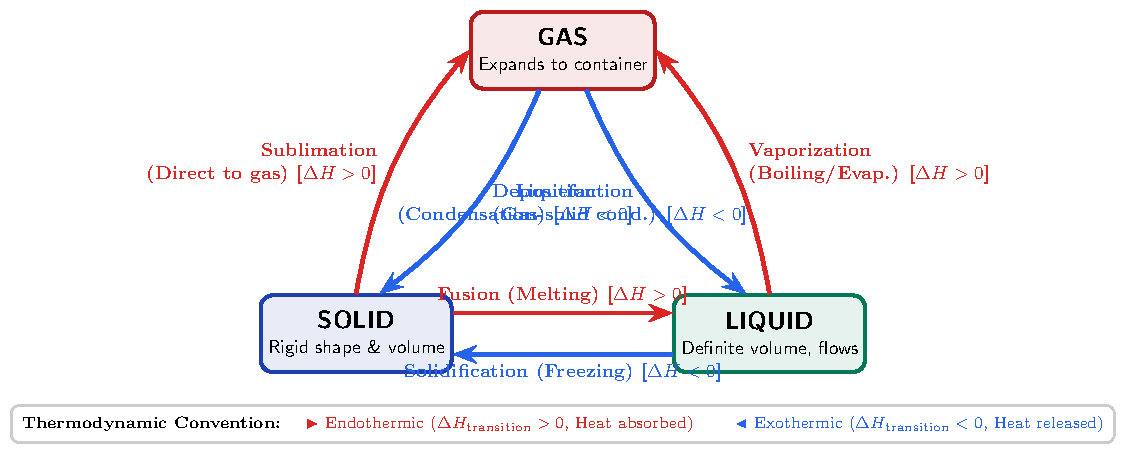
\includegraphics[width=0.88\textwidth]{figures/01_phase_transitions.pdf}
\caption{The thermodynamic cycle of macroscopic phase transitions. Red arrows denote endothermic transitions ($\Delta H > 0$, requiring thermal energy input); blue arrows denote exothermic transitions ($\Delta H < 0$, releasing thermal energy to the surroundings).}
\label{fig:phase_transitions}
\end{figure}

The six canonical phase transformations are classified in complementary forward-reverse pairs:
\begin{enumerate}[leftmargin=1.5em,itemsep=4pt]
  \item \textbf{Solid $\longleftrightarrow$ Liquid:}
  \begin{itemize}[leftmargin=1.2em]
    \item \textbf{Fusion (Melting):} Solid $\to$ Liquid. \emph{Endothermic} ($\Delta H_{\text{fus}} > 0$). Requires latent heat of fusion.
    \item \textbf{Solidification (Freezing):} Liquid $\to$ Solid. \emph{Exothermic} ($\Delta H_{\text{solid}} = -\Delta H_{\text{fus}} < 0$).
    \item At standard pressure ($P = 1\ \mathrm{atm}$), pure water melts/freezes at $T_{\text{fus}} = 0^\circ\mathrm{C}$ ($273.15\ \mathrm{K}$); pure iron melts at $T_{\text{fus}} = 1538^\circ\mathrm{C}$ ($1811\ \mathrm{K}$).
  \end{itemize}
  \item \textbf{Liquid $\longleftrightarrow$ Gas:}
  \begin{itemize}[leftmargin=1.2em]
    \item \textbf{Vaporization:} Liquid $\to$ Gas (by slow evaporation at the surface or boiling throughout the bulk). \emph{Endothermic} ($\Delta H_{\text{vap}} > 0$).
    \item \textbf{Liquefaction (Condensation):} Gas $\to$ Liquid. \emph{Exothermic} ($\Delta H_{\text{liq}} = -\Delta H_{\text{vap}} < 0$).
    \item Pure water boils at $T_{\text{vap}} = 100^\circ\mathrm{C}$ ($373.15\ \mathrm{K}$) at $1\ \mathrm{atm}$.
  \end{itemize}
  \item \textbf{Solid $\longleftrightarrow$ Gas:}
  \begin{itemize}[leftmargin=1.2em]
    \item \textbf{Sublimation:} Direct solid $\to$ gas transition without passing through an intermediate liquid phase. \emph{Endothermic} ($\Delta H_{\text{sub}} > 0$). Characteristic of dry ice ($\mathrm{CO_2}$ solid sublimates at $-78.5^\circ\mathrm{C}$) and iodine crystals ($\mathrm{I_2}$).
    \item \textbf{Deposition (Gas-Solid Condensation):} Direct gas $\to$ solid transition. \emph{Exothermic} ($\Delta H_{\text{dep}} = -\Delta H_{\text{sub}} < 0$). Observed in frost formation from water vapor.
  \end{itemize}
\end{enumerate}

By Hess's law of thermodynamic state functions, the enthalpy of sublimation equals the exact sum of fusion and vaporization enthalpies at identical temperature and pressure:
\begin{equation}
\Delta H_{\text{sub}} = \Delta H_{\text{fus}} + \Delta H_{\text{vap}}.
\end{equation}

\section{Physical vs. Chemical Changes and Lavoisier's Conservation Law}

\begin{definitionbox}{Physical Change vs. Chemical Change}
\begin{itemize}[leftmargin=1.5em,itemsep=3pt]
  \item \textbf{Physical Change:} A transformation that modifies the physical appearance, dimensions, or aggregation state of a substance, but leaves its \textbf{molecular and atomic constitution strictly invariant}. No chemical bonds are broken or created (e.g., dissolution of sugar in water, pulverization of rock salt, condensation of steam).
  \item \textbf{Chemical Change (Chemical Reaction):} A fundamental transformation wherein initial substances (\textbf{reactants}) are converted into chemically distinct new substances (\textbf{products}) via the rupture and reformation of electronic and chemical bonds.
\end{itemize}
\end{definitionbox}

Experimental indicators of a chemical transformation include:
\begin{enumerate}[leftmargin=1.5em,itemsep=2pt]
  \item Evolution of a gaseous product (effervescence),
  \item Formation of an insoluble solid precipitate ($\downarrow$),
  \item Permanent color change of the solution or solid matrix,
  \item Exothermic heat release ($\Delta H < 0$) or endothermic cooling ($\Delta H > 0$),
  \item Emission of electromagnetic radiation (chemiluminescence or flames).
\end{enumerate}

\begin{historicalbox}{Antoine-Laurent de Lavoisier: Father of Modern Chemistry}
\begin{minipage}{0.28\textwidth}
\centering
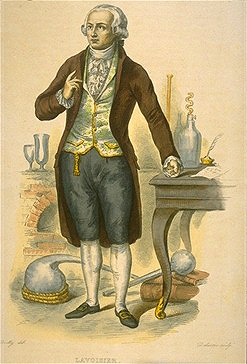
\includegraphics[width=0.92\textwidth]{images/lavoisier.jpg}
\captionof{figure}{Antoine-Laurent de Lavoisier (1743--1794), portrait by Jacques-Louis David (1788, Metropolitan Museum of Art).}
\end{minipage}\hfill
\begin{minipage}{0.68\textwidth}
In his revolutionary 1789 treatise \emph{Traité Élémentaire de Chimie}, French chemist Antoine-Laurent de Lavoisier dismantled the centuries-old phlogiston dogma. Utilizing closed hermetic combustion chambers and ultra-precise balance scales, Lavoisier demonstrated that during the combustion of phosphorus and sulfur in air, the weight gained by the solids was exactly equal to the weight lost by the surrounding air.

Lavoisier formulated the foundational axiom of chemistry: ``\emph{Rien ne se perd, rien ne se crée, tout se transforme}'' (Nothing is lost, nothing is created, everything is transformed), proving that chemical reactions represent a conserved atomic rearrangement.
\end{minipage}
\end{historicalbox}

\begin{lawbox}{Lavoisier's Law of Conservation of Mass}
In any closed chemical or physical system, the total mass remains strictly invariant throughout any transformation:
\begin{equation}
\sum m_{\text{reactants consumed}} = \sum m_{\text{products formed}}.
\end{equation}
In stoichiometric form for a general chemical reaction $\sum_i \nu_i \mathrm{R}_i \to \sum_j \nu_j' \mathrm{P}_j$:
\begin{equation}
\sum_i \nu_i M(\mathrm{R}_i) = \sum_j \nu_j' M(\mathrm{P}_j),
\end{equation}
which implies the strict, simultaneous conservation of every individual chemical element $X$.
\end{lawbox}

\section{Atoms, Molecules, and the Mole Concept}

\subsection{The Atomic and Molecular Nature of Matter}
\begin{itemize}[leftmargin=1.5em,itemsep=3pt]
  \item \textbf{The Atom:} The fundamental building block of chemical elements. An atom is electrically neutral, consisting of an ultra-dense, positively charged nucleus ($r_n \sim 10^{-14}\ \mathrm{m}$) surrounded by a diffuse cloud of negatively charged electrons ($r_{\text{atom}} \sim 10^{-10}\ \mathrm{m}$).
  \item \textbf{The Molecule:} A discrete, electrically neutral group of two or more atoms held together in a fixed spatial stoichiometry by covalent bonds (e.g., $\mathrm{H_2O, CO_2, NH_3}$).
\end{itemize}

\begin{historicalbox}{John Dalton and the Chemical Atomic Theory}
\begin{minipage}{0.28\textwidth}
\centering
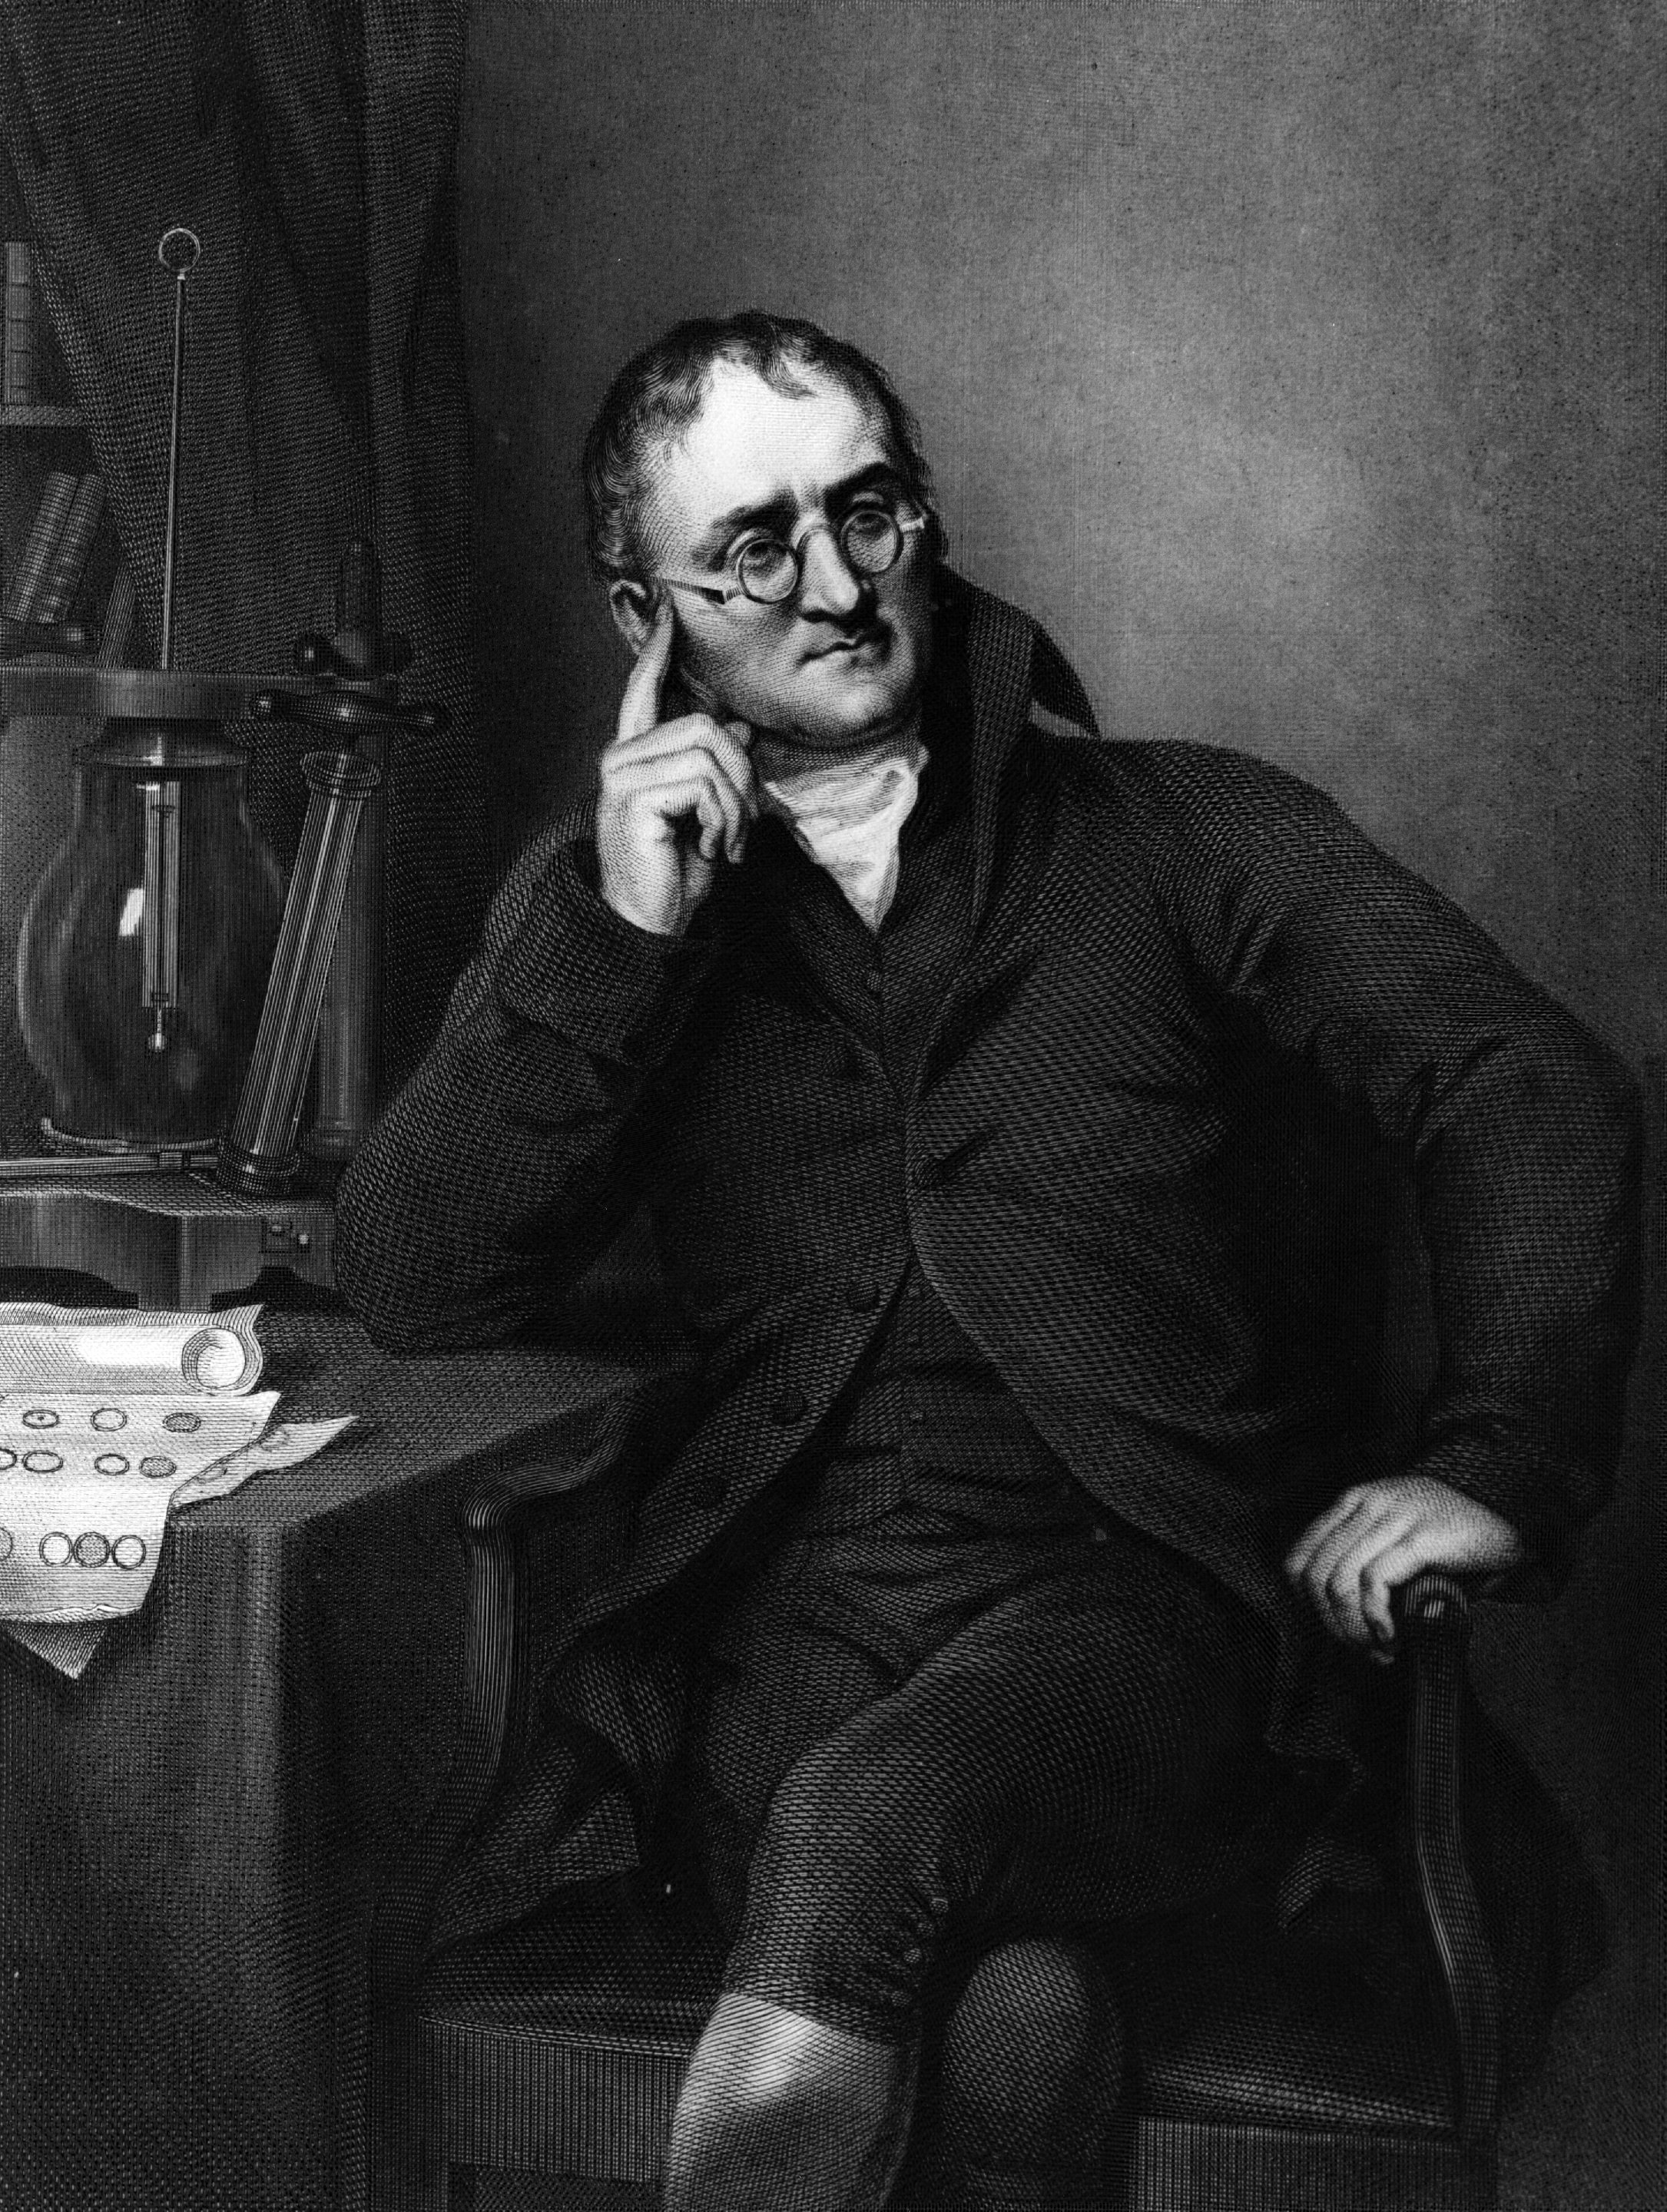
\includegraphics[width=0.92\textwidth]{images/dalton.jpg}
\captionof{figure}{John Dalton (1766--1844), portrait by Thomas Phillips (1835, National Portrait Gallery, London).}
\end{minipage}\hfill
\begin{minipage}{0.68\textwidth}
In 1803, English chemist and meteorologist John Dalton proposed the first modern atomic theory. Observing that elements always combine in fixed, simple integer mass ratios (the Law of Definite Proportions and the Law of Multiple Proportions), Dalton deduced that:
\begin{enumerate}[leftmargin=1.2em,itemsep=2pt]
  \item All matter consists of indivisible, indestructible particles called atoms;
  \item All atoms of a given element possess identical chemical properties and mass;
  \item Chemical compounds are formed when atoms of different elements combine in simple numerical ratios ($1:1, 1:2, 2:3$, etc.).
\end{enumerate}
\end{minipage}
\end{historicalbox}

\subsection{The Mole and Avogadro's Constant}

Because individual atoms have minuscule masses ($\sim 10^{-26}\ \mathrm{kg}$), macroscopic laboratory experiments require a bridge linking macroscopic mass measurements to microscopic particle counts.

\begin{definitionbox}{The Mole and Avogadro's Constant}
The \textbf{mole} (symbol: $\mathrm{mol}$) is the SI base unit for the \textbf{amount of substance} ($n$). One mole contains exactly $6.022\,140\,76 \times 10^{23}$ elementary entities (atoms, molecules, ions, electrons, or other specified groups of particles).
This defining numerical constant is \textbf{Avogadro's constant}:
\begin{equation}
N_A = 6.022\,140\,76 \times 10^{23}\ \mathrm{mol^{-1}} \quad (\text{often rounded to } 6.023 \times 10^{23}\ \mathrm{mol^{-1}}).
\end{equation}
The total number of particles $N$ in a sample of substance amount $n$ is:
\begin{equation}
N = n \cdot N_A \iff n = \frac{N}{N_A}.
\end{equation}
\end{definitionbox}

\begin{historicalbox}{Amedeo Avogadro and the Molecular Hypothesis}
\begin{minipage}{0.28\textwidth}
\centering
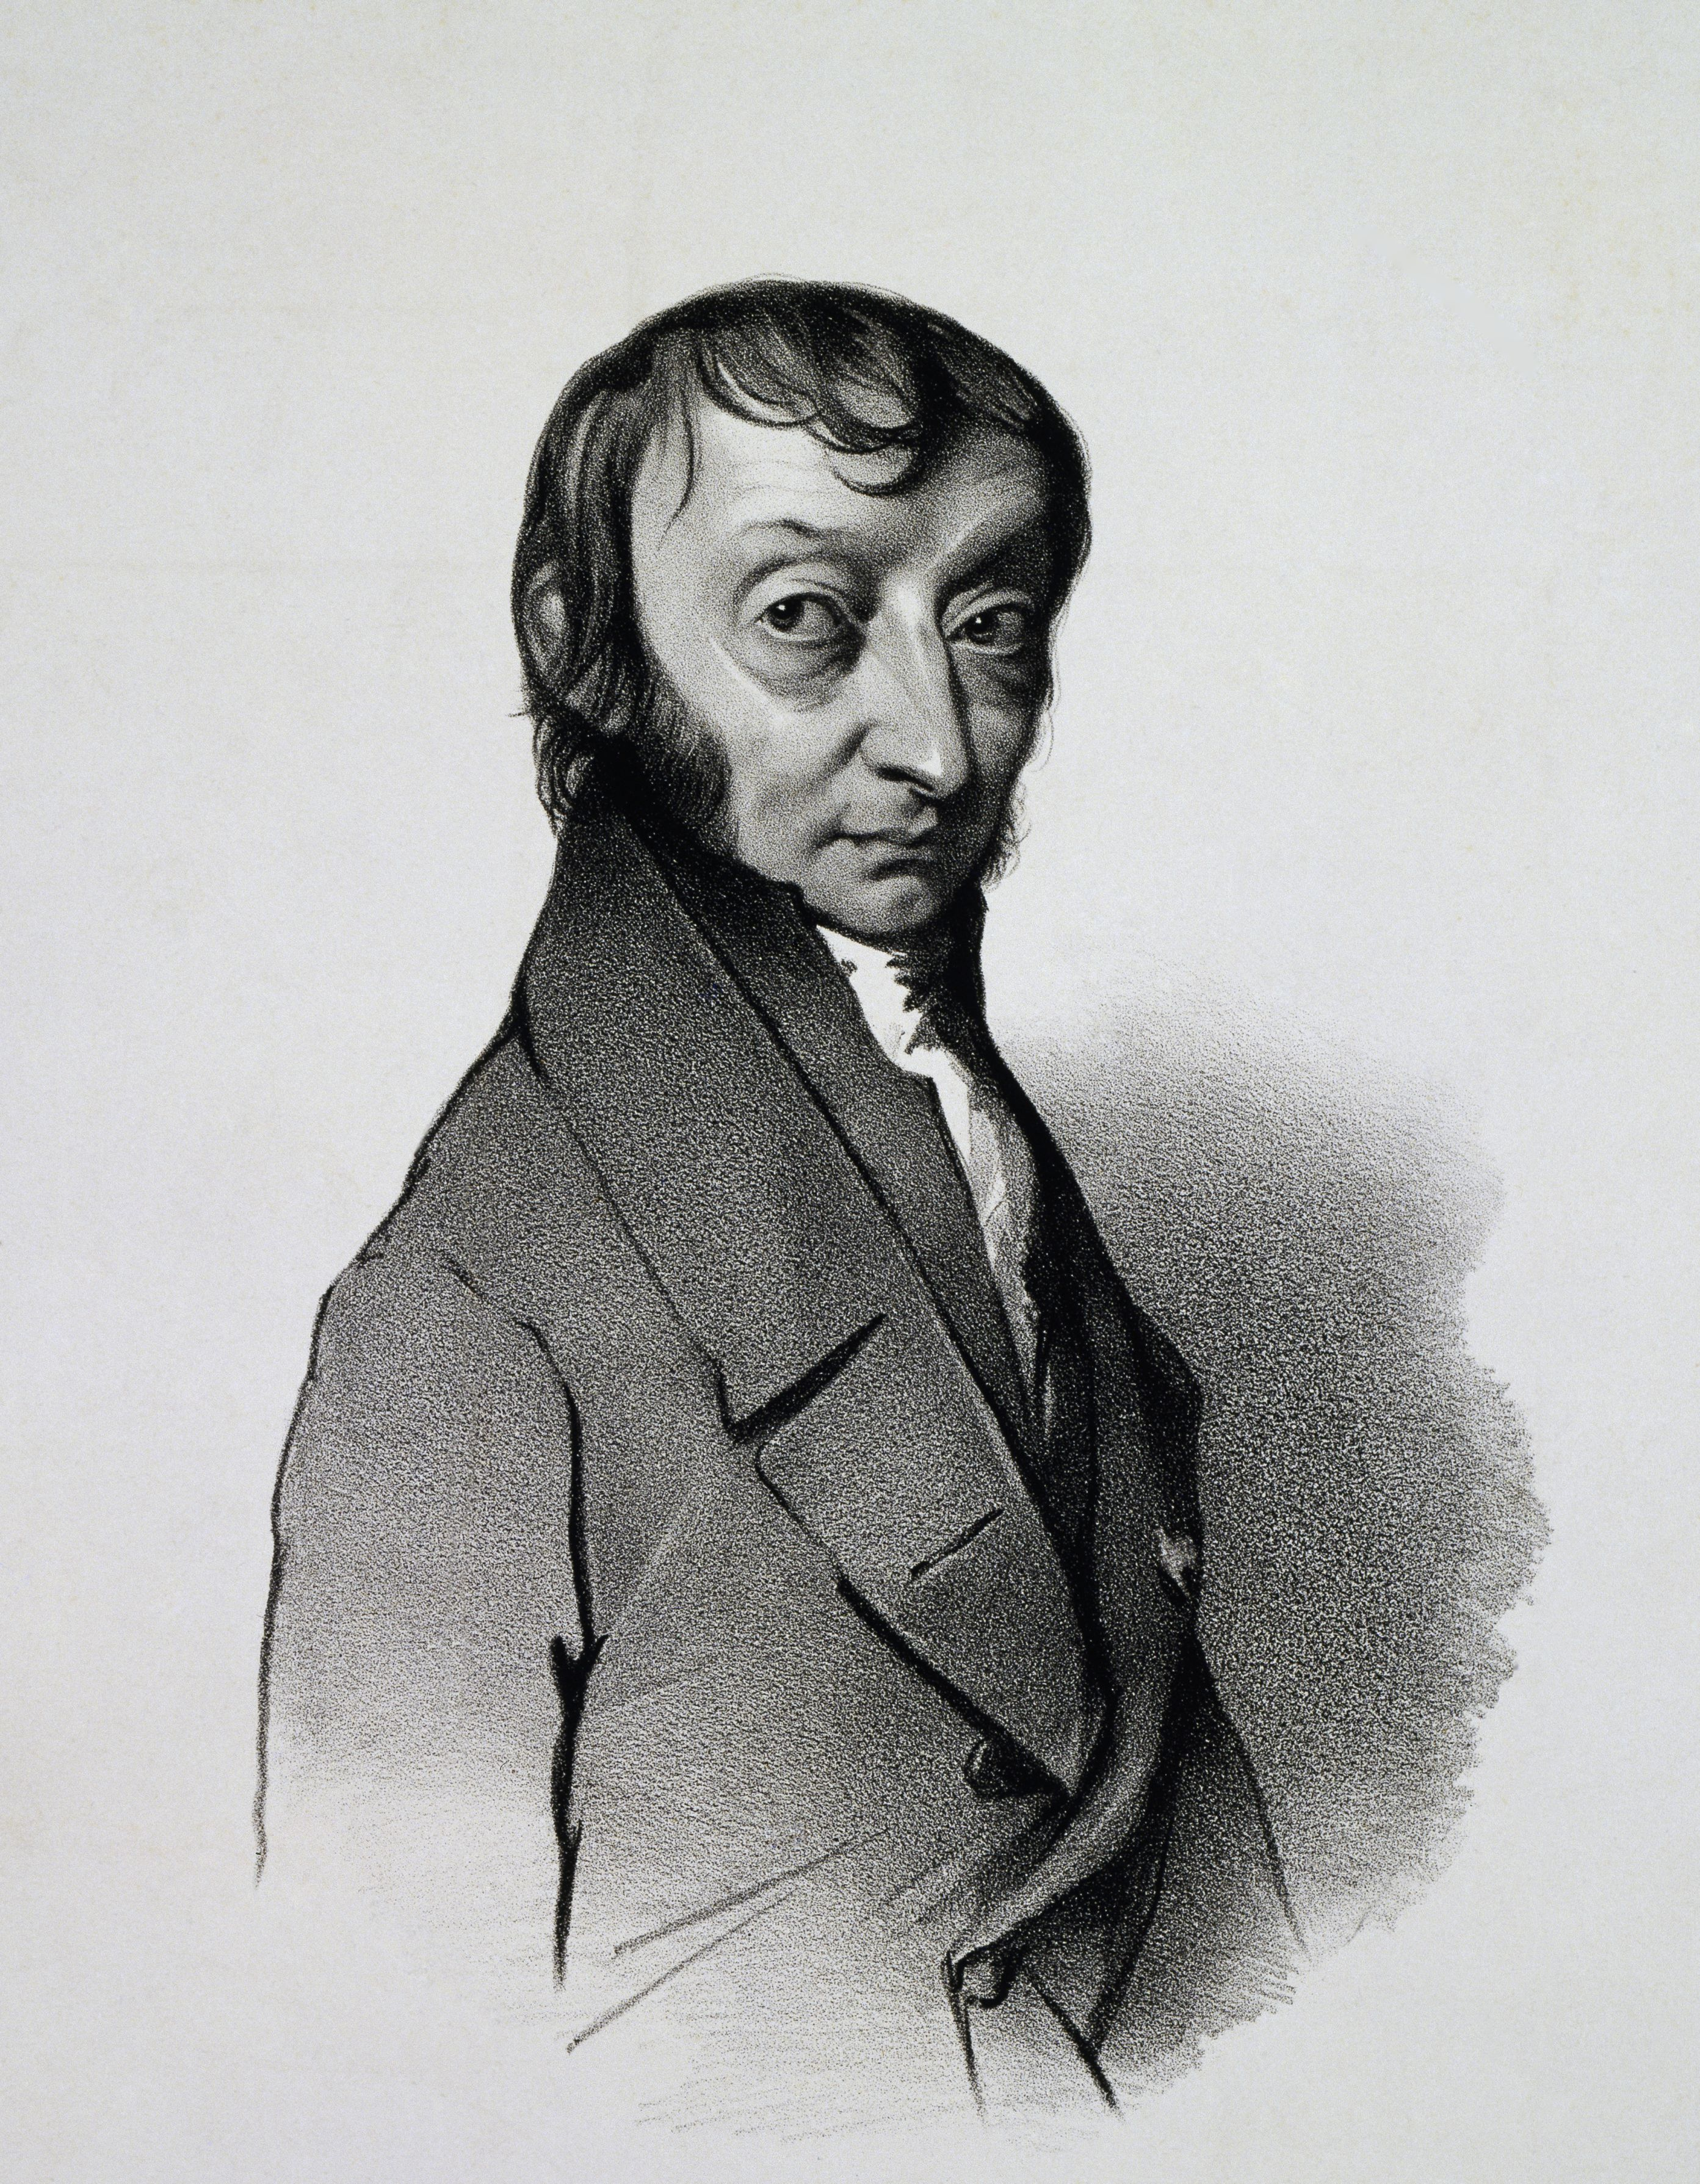
\includegraphics[width=0.92\textwidth]{images/avogadro.jpg}
\captionof{figure}{Amedeo Avogadro (1776--1856), contemporary Italian engraving.}
\end{minipage}\hfill
\begin{minipage}{0.68\textwidth}
In 1811, Italian physicist Amedeo Avogadro published his historic hypothesis: ``\emph{Equal volumes of all gases, measured at the same temperature and pressure, contain equal numbers of molecules}.''

Avogadro correctly distinguished between fundamental atoms and multi-atom molecules, explaining Gay-Lussac's law of combining volumes (e.g., $2\ \text{volumes of } \mathrm{H_2} + 1\ \text{volume of } \mathrm{O_2} \to 2\ \text{volumes of steam } \mathrm{H_2O}$). His brilliant insight was finally vindicated in 1860 by Stanislao Cannizzaro at the Karlsruhe Congress.
\end{minipage}
\end{historicalbox}

\section{Mass and Volume Metrics}

\subsection{1. The Unified Atomic Mass Unit}
Because the mass of an atom is inconveniently small in kilograms, the international scientific community defines an atomic-scale unit referenced to the carbon-12 isotope ($^{12}\mathrm{C}$):

\begin{definitionbox}{Unified Atomic Mass Unit (u or amu)}
The \textbf{unified atomic mass unit} ($1\ \mathrm{u}$) is defined as exactly $\frac{1}{12}$ of the mass of a single unbound, neutral Carbon-12 atom ($^{12}\mathrm{C}$) in its electronic and nuclear ground state:
\begin{equation}
1\ \mathrm{u} \eqdef \frac{1}{12} m(^{12}\mathrm{C}) = \frac{1}{N_A} \approx 1.660\,539 \times 10^{-24}\ \mathrm{g} = 1.660\,539 \times 10^{-27}\ \mathrm{kg}.
\end{equation}
\end{definitionbox}

\subsection{2. Molar Mass}
\begin{definitionbox}{Molar Mass ($M$)}
The \textbf{molar mass} $M$ of a substance is the mass of one mole ($N_A$ particles) of that substance:
\begin{equation}
M \eqdef \frac{m}{n}, \qquad [M] = \mathrm{g\cdot mol^{-1}} \quad (\text{or } \mathrm{kg\cdot mol^{-1}}).
\end{equation}
\begin{itemize}[leftmargin=1.5em,itemsep=2pt]
  \item \textbf{Atomic Molar Mass $M(X)$:} Mass of 1 mole of free atoms of element $X$. Numerically identical to its relative atomic mass in $\mathrm{u}$ (e.g., $M(\mathrm{H}) = 1.008\ \mathrm{g/mol}$, $M(\mathrm{C}) = 12.011\ \mathrm{g/mol}$, $M(\mathrm{O}) = 15.999\ \mathrm{g/mol}$, $M(\mathrm{S}) = 32.06\ \mathrm{g/mol}$).
  \item \textbf{Molecular Molar Mass $M(\mathrm{A}_x \mathrm{B}_y)$:} The stoichiometric sum of the atomic molar masses of all constituent atoms in the chemical formula:
  \begin{equation}
  M(\mathrm{A}_x \mathrm{B}_y) = x \cdot M(\mathrm{A}) + y \cdot M(\mathrm{B}).
  \end{equation}
  \emph{Example:} For water ($\mathrm{H_2O}$):
  \[
  M(\mathrm{H_2O}) = 2 M(\mathrm{H}) + M(\mathrm{O}) = 2(1.008) + 15.999 = 18.015\ \mathrm{g\cdot mol^{-1}}.
  \]
\end{itemize}
\end{definitionbox}

\subsection{3. Molar Volume of Gases}
\begin{definitionbox}{Molar Volume ($V_m$)}
The \textbf{molar volume} $V_m$ of a chemical substance is the spatial volume occupied by one mole of that substance in a specified thermodynamic state $(T, P)$:
\begin{equation}
V_m \eqdef \frac{V}{n}, \qquad [V_m] = \mathrm{L\cdot mol^{-1}} \quad (\text{or } \mathrm{m^3\cdot mol^{-1}}).
\end{equation}
From the Ideal Gas Law ($P V = n R T$):
\begin{equation}
V_m = \frac{R T}{P}.
\end{equation}
Under **Standard Temperature and Pressure (STP / CNTP)**, defined as $T_0 = 0^\circ\mathrm{C} = 273.15\ \mathrm{K}$ and $P_0 = 1\ \mathrm{atm} = 101\,325\ \mathrm{Pa}$:
\begin{equation}
V_m = \frac{(8.31446\ \mathrm{J\cdot mol^{-1}\cdot K^{-1}})(273.15\ \mathrm{K})}{101\,325\ \mathrm{Pa}} = 0.022\,414\ \mathrm{m^3\cdot mol^{-1}} = 22.414\ \mathrm{L\cdot mol^{-1}}.
\end{equation}
\end{definitionbox}

\begin{lawbox}{Universal Stoichiometric Master Equation}
For any pure chemical sample of mass $m$, particle count $N$, and gas volume $V_{\text{gas}}$ at STP:
\begin{equation}
n = \frac{m}{M} = \frac{N}{N_A} = \frac{V_{\text{gas}}}{V_m}.
\end{equation}
\end{lawbox}

\section{Classification of Matter and Solution Chemistry}

\subsection{Pure Substances and Mixtures}
Matter is universally partitioned into two great classes:

\begin{figure}[htbp]
\centering
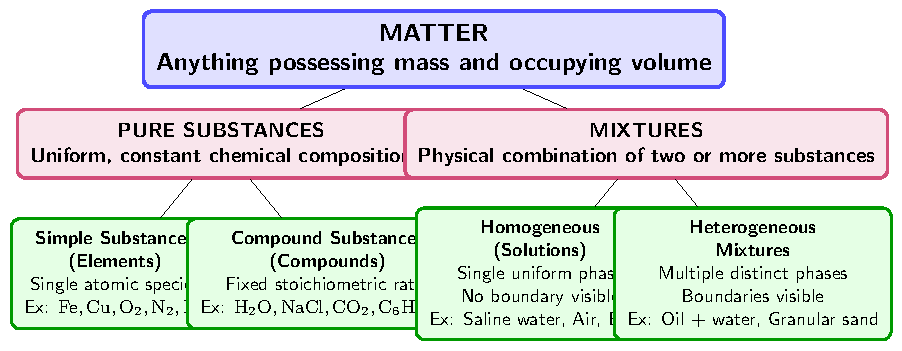
\includegraphics[width=0.88\textwidth]{figures/02_matter_classification.pdf}
\caption{The hierarchical classification of matter into pure substances (simple elements and compound species) and mixtures (homogeneous solutions and heterogeneous multi-phase systems).}
\label{fig:matter_classification}
\end{figure}

\begin{enumerate}[leftmargin=1.5em,itemsep=3pt]
  \item \textbf{Pure Substances:} Possess a uniform, definite, and invariant chemical composition throughout.
  \begin{itemize}[leftmargin=1.2em]
    \item \textbf{Simple Substances (Elements):} Formed from atoms of a single chemical element. Cannot be decomposed into simpler substances by chemical reactions (e.g., metals $\mathrm{Fe, Cu, Al}$; non-metal allotropes $\mathrm{O_2, O_3, C_{\text{graphite}}, S_8}$).
    \item \textbf{Compound Substances (Compounds):} Formed from two or more distinct elements chemically bound in fixed, constant stoichiometric proportions (e.g., $\mathrm{H_2O, NaCl, CO_2, H_2SO_4}$). Can be broken down into constituent elements by chemical reactions.
  \end{itemize}
  \item \textbf{Mixtures:} Physical combinations of two or more pure substances that do not react chemically. The components retain their individual chemical identities and can be separated by physical methods (distillation, filtration, centrifugation, chromatography).
  \begin{itemize}[leftmargin=1.2em]
    \item \textbf{Homogeneous Mixtures (Solutions):} The components are dispersed at the molecular or ionic scale, forming a single uniform macroscopic phase. No constituent boundaries are distinguishable, even under optical microscopy (e.g., sugar dissolved in water, air, bronze alloy).
    \item \textbf{Heterogeneous Mixtures:} Possess two or more distinct phases separated by visible interfaces. Constituents can be visually distinguished (e.g., oil and water, granite rock, suspension of clay in water).
  \end{itemize}
\end{enumerate}

\subsection{Solutions, Solutes, and Solvents}

\begin{definitionbox}{Solution Architecture}
A \textbf{solution} is a homogeneous mixture formed by dissolving one or more minor chemical species (\textbf{solutes}) into a predominant dispersing medium (\textbf{solvent}):
\begin{equation}
\text{Solution} = \text{Solvent} + \sum \text{Solutes}.
\end{equation}
When the solvent is liquid water ($\mathrm{H_2O}$), the system is designated an \textbf{aqueous solution}.
\end{definitionbox}

\begin{itemize}[leftmargin=1.5em,itemsep=3pt]
  \item \textbf{Solubility Limit and Saturation:} A solution is said to be \textbf{saturated} when the dissolved solute concentration has reached thermodynamic equilibrium with undissolved solute at a given temperature. Any additional solute cannot dissolve and settles as a solid precipitate ($\downarrow$), indicating \textbf{supersaturation}.
  \item \textbf{The Dilution Process:} Dilution consists of adding pure solvent to a pre-existing concentrated solution (\textbf{mother solution}), producing a lower-concentration \textbf{daughter solution}.
\end{itemize}

\begin{figure}[htbp]
\centering
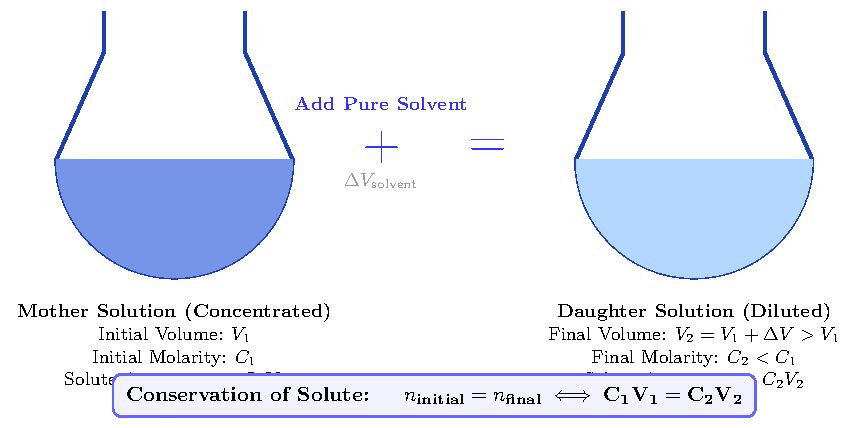
\includegraphics[width=0.88\textwidth]{figures/03_solution_dilution.pdf}
\caption{The principle of dilution. Adding pure solvent increases total volume from $V_1$ to $V_2$ while the absolute amount of dissolved solute remains strictly conserved ($n_1 = n_2 \implies C_1 V_1 = C_2 V_2$).}
\label{fig:solution_dilution}
\end{figure}

\begin{lawbox}{The Fundamental Dilution Invariant}
Because adding pure solvent adds strictly zero solute, the total amount of solute $n$ is an invariant of the dilution process:
\begin{equation}
n_{\text{initial}} = n_{\text{final}} \iff \mathbf{C_1 V_1 = C_2 V_2} \quad (\text{or } C_i V_i = C_f V_f).
\end{equation}
The dimensionless \textbf{dilution factor} $F$ is defined as:
\begin{equation}
F \eqdef \frac{V_2}{V_1} = \frac{C_1}{C_2} > 1.
\end{equation}
\end{lawbox}

\section{Mathematical Formulations of Solution Concentrations}

In chemistry, the composition of a solution is quantified through four standard concentration measures:

\subsection{1. Molarity (Molar Concentration, $C_M$ or $[\mathrm{X}]$)}
The molar concentration represents the amount of solute per unit volume of solution:
\begin{equation}
C_M \eqdef \frac{n_{\text{solute}}}{V_{\text{solution}}} = \frac{m_{\text{solute}}}{M_{\text{solute}} \cdot V_{\text{solution}}}, \qquad [C_M] = \mathrm{mol\cdot L^{-1}} = \mathrm{mol\cdot dm^{-3}} \equiv \mathrm{M}.
\end{equation}

\subsection{2. Mass Concentration (Titre or Mass Content, $C_m$)}
The mass concentration represents the mass of solute dissolved per unit volume of solution:
\begin{equation}
C_m \eqdef \frac{m_{\text{solute}}}{V_{\text{solution}}}, \qquad [C_m] = \mathrm{g\cdot L^{-1}}.
\end{equation}

\begin{lawbox}{Direct Relationship Between $C_m$ and $C_M$}
Multiplying molarity by the molar mass of the solute yields mass concentration directly:
\begin{equation}
C_m = \frac{m}{V} = \frac{n \cdot M}{V} = \left(\frac{n}{V}\right) M = \mathbf{C_M \cdot M}.
\end{equation}
\end{lawbox}

\subsection{3. Molality ($m$ or $b$)}
Molality expresses the amount of solute dissolved per unit mass of \textbf{pure solvent}:
\begin{equation}
m \eqdef \frac{n_{\text{solute}}}{m_{\text{solvent (in kg)}}}, \qquad [m] = \mathrm{mol\cdot kg^{-1}}.
\end{equation}
\emph{Crucial thermodynamic advantage:} Unlike molarity (which changes with temperature due to liquid thermal expansion $\dd V/\dd T \neq 0$), \textbf{molality is strictly independent of temperature and pressure}, making it the mandatory metric in colligative property thermodynamics (boiling-point elevation and freezing-point depression).

\subsection{4. Mass Fraction ($w$) and Percentage Purity ($P\%$)}
The mass fraction is the ratio of solute mass to total solution mass:
\begin{equation}
w \eqdef \frac{m_{\text{solute}}}{m_{\text{solution}}}, \qquad P\% \eqdef w \times 100\% = \frac{m_{\text{solute}}}{m_{\text{solution}}} \times 100\%.
\end{equation}
Given a concentrated commercial liquid solution of mass percentage $P\%$, solute molar mass $M$ ($\mathrm{g/mol}$), and relative density $d$ (specific gravity relative to water, $\rho = d\ \mathrm{g\cdot mL^{-1}} = 1000\,d\ \mathrm{g\cdot L^{-1}}$), the molarity is derived rigorously by considering $1\ \mathrm{L}$ ($1000\ \mathrm{mL}$) of solution:
\[
m_{\text{solution}} = 1000 \cdot d\ \mathrm{g}, \qquad m_{\text{solute}} = m_{\text{solution}} \times \frac{P\%}{100} = 10 \cdot d \cdot P\%\ \mathrm{g}.
\]
Dividing by molar mass $M$:
\begin{lawbox}{Molarity of Commercial Concentrated Reagents}
\begin{equation}
C_M = \frac{10 \cdot P\% \cdot d}{M}.
\end{equation}
\end{lawbox}

\subsection{5. Normality ($N$) and the Concept of Gram-Equivalents}

\begin{definitionbox}{Normality (Equivalent Concentration)}
The \textbf{normality} $N$ of a chemical solution is the number of **gram-equivalents** ($\mathrm{eq}$) of solute dissolved per liter of solution:
\begin{equation}
N \eqdef \frac{\text{Number of Gram-Equivalents}}{V_{\text{solution (L)}}}.
\end{equation}
The normality is related to molarity through the dimensionless stoichiometric **valence factor** $Z$:
\begin{equation}
\mathbf{N = C_M \cdot Z}.
\end{equation}
The unit of normality is the **equivalent per liter** ($\mathrm{eq\cdot L^{-1}}$ or $\mathrm{N}$).
\end{definitionbox}

The physical definition of the valence factor $Z$ depends strictly on the reaction context:

\begin{center}
\renewcommand{\arraystretch}{1.35}
\begin{tabular}{@{}lll@{}}
\toprule
\textbf{Reaction Context} & \textbf{Physical Definition of Valence Factor $Z$} & \textbf{Canonical Examples} \\
\midrule
\textbf{Acids} & Number of exchangeable acidic protons $\mathrm{H}^+$ & $\mathrm{HCl}: Z = 1 \implies N = C_M$ \\
& per formula unit & $\mathrm{H_2SO_4}: Z = 2 \implies N = 2 C_M$ \\
& & $\mathrm{H_3PO_4}: Z = 3 \implies N = 3 C_M$ \\
\midrule
\textbf{Bases} & Number of exchangeable hydroxide ions $\mathrm{OH}^-$ & $\mathrm{NaOH}: Z = 1 \implies N = C_M$ \\
& (or protons neutralized) per formula unit & $\mathrm{Ca(OH)_2}: Z = 2 \implies N = 2 C_M$ \\
& & $\mathrm{Al(OH)_3}: Z = 3 \implies N = 3 C_M$ \\
\midrule
\textbf{Salts} & Total positive charge: & $\mathrm{NaCl}: Z = 1 \times (+1) = 1$ \\
& (number of metal cations) $\times$ (cation charge) & $\mathrm{Na_2SO_4}: Z = 2 \times (+1) = 2$ \\
& & $\mathrm{Al_2(SO_4)_3}: Z = 2 \times (+3) = 6$ \\
\midrule
\textbf{Redox Reactions} & Number of electrons exchanged ($n_{e^-}$) & $\mathrm{MnO_4^-} \to \mathrm{Mn^{2+}} \ (5e^-): Z = 5$ \\
& in the specific half-reaction & $\mathrm{Cr_2O_7^{2-}} \to 2\mathrm{Cr^{3+}} \ (6e^-): Z = 6$ \\
& & $\mathrm{Fe^{2+}} \to \mathrm{Fe^{3+}} \ (1e^-): Z = 1$ \\
\bottomrule
\end{tabular}
\end{center}

\begin{lawbox}{The Equivalence Principle in Volumetric Titrations}
At the stoichiometric equivalence point of any quantitative volumetric titration between species 1 and species 2 (whether acid-base, precipitation, or redox), the number of reacting equivalents is identically equal:
\begin{equation}
N_1 V_1 = N_2 V_2.
\end{equation}
This universal equivalence law is the operational reason chemists introduced normality: it eliminates the need to carry stoichiometric coefficients explicitly during titration calculations.
\end{lawbox}

\begin{cautionbox}[Common Pitfall: Normality is Reaction-Dependent]
Unlike molarity, which is an intrinsic property of a prepared bottle, **normality depends on the reaction in which the substance participates**. For instance, in an acidic medium, potassium permanganate reacts via:
\[
\mathrm{MnO_4^-} + 8\mathrm{H}^+ + 5e^- \longrightarrow \mathrm{Mn}^{2+} + 4\mathrm{H_2O} \implies Z = 5 \implies N = 5 C_M.
\]
However, in a neutral or alkaline medium, it reduces only to manganese dioxide:
\[
\mathrm{MnO_4^-} + 2\mathrm{H_2O} + 3e^- \longrightarrow \mathrm{MnO_2} + 4\mathrm{OH}^- \implies Z = 3 \implies N = 3 C_M.
\]
A single $0.1\ \mathrm{M}\ \mathrm{KMnO_4}$ solution is $0.5\ \mathrm{N}$ in acid, but $0.3\ \mathrm{N}$ in base!
\end{cautionbox}

\section{Comprehensive Worked Examples}

\begin{workedexample}{Stoichiometric Combustion and Lavoisier Mass Conservation}
Propane gas ($\mathrm{C_3H_8}$) undergoes complete combustion with gaseous oxygen ($\mathrm{O_2}$) to produce carbon dioxide ($\mathrm{CO_2}$) and liquid water ($\mathrm{H_2O}$). A laboratory burner consumes $44.10\ \mathrm{g}$ of propane.
\begin{enumerate}[leftmargin=1.4em,itemsep=3pt]
  \item Write the balanced chemical equation and determine the stoichiometric mole ratios.
  \item Calculate the amount of substance (in moles) of propane consumed.
  \item Determine the theoretical mass of oxygen consumed, and the volume of pure oxygen and air required at STP ($V_m = 22.414\ \mathrm{L\cdot mol^{-1}}$, air is $21.0\%$ $\mathrm{O_2}$ by volume).
  \item Calculate the masses of $\mathrm{CO_2}$ and $\mathrm{H_2O}$ formed, and explicitly verify Lavoisier's conservation of mass.
\end{enumerate}

\paragraph{Solution.}
\textbf{1. Balanced Chemical Reaction:}\\
Balancing carbon ($3\ \mathrm{C}$), hydrogen ($8\ \mathrm{H} \to 4\ \mathrm{H_2O}$), and oxygen ($3 \times 2 + 4 \times 1 = 10\ \mathrm{O} \to 5\ \mathrm{O_2}$):
\[
\mathrm{C_3H_8(g)} + 5\,\mathrm{O_2(g)} \longrightarrow 3\,\mathrm{CO_2(g)} + 4\,\mathrm{H_2O(l)}.
\]

\textbf{2. Amount of Propane Consumed:}\\
The molar mass of propane is $M(\mathrm{C_3H_8}) = 3(12.011) + 8(1.008) = 36.033 + 8.064 = 44.097\ \mathrm{g\cdot mol^{-1}}$.
\[
n(\mathrm{C_3H_8}) = \frac{m}{M} = \frac{44.10\ \mathrm{g}}{44.097\ \mathrm{g\cdot mol^{-1}}} \approx 1.000\ \mathrm{mol}.
\]

\textbf{3. Oxygen Requirements:}\\
From the stoichiometric ratio $\frac{n(\mathrm{O_2})}{n(\mathrm{C_3H_8})} = \frac{5}{1}$:
\[
n(\mathrm{O_2}) = 5 \times 1.000 = 5.000\ \mathrm{mol}.
\]
The molar mass of oxygen is $M(\mathrm{O_2}) = 2(15.999) = 31.998\ \mathrm{g\cdot mol^{-1}}$.
The mass of oxygen consumed is:
\[
m(\mathrm{O_2}) = n \times M = 5.000\ \mathrm{mol} \times 31.998\ \mathrm{g\cdot mol^{-1}} = 159.99\ \mathrm{g} \approx 160.0\ \mathrm{g}.
\]
The volume of pure $\mathrm{O_2}$ gas required at STP is:
\[
V(\mathrm{O_2}) = n \times V_m = 5.000\ \mathrm{mol} \times 22.414\ \mathrm{L\cdot mol^{-1}} = 112.07\ \mathrm{L}.
\]
The corresponding volume of ambient air required is:
\[
V(\text{air}) = \frac{V(\mathrm{O_2})}{0.210} = \frac{112.07\ \mathrm{L}}{0.210} \approx 533.7\ \mathrm{L}.
\]

\textbf{4. Products Formed and Verification of Lavoisier Conservation:}\\
From the stoichiometry:
\begin{itemize}[leftmargin=1.5em,itemsep=3pt]
  \item Carbon dioxide: $n(\mathrm{CO_2}) = 3 \times 1.000 = 3.000\ \mathrm{mol}$.
  \[
  M(\mathrm{CO_2}) = 12.011 + 2(15.999) = 44.009\ \mathrm{g\cdot mol^{-1}}.
  \]
  \[
  m(\mathrm{CO_2}) = 3.000 \times 44.009 = 132.03\ \mathrm{g}.
  \]
  \item Water: $n(\mathrm{H_2O}) = 4 \times 1.000 = 4.000\ \mathrm{mol}$.
  \[
  M(\mathrm{H_2O}) = 2(1.008) + 15.999 = 18.015\ \mathrm{g\cdot mol^{-1}}.
  \]
  \[
  m(\mathrm{H_2O}) = 4.000 \times 18.015 = 72.06\ \mathrm{g}.
  \]
\end{itemize}
Total mass of reactants:
\[
\sum m_{\text{reactants}} = m(\mathrm{C_3H_8}) + m(\mathrm{O_2}) = 44.10\ \mathrm{g} + 159.99\ \mathrm{g} = 204.09\ \mathrm{g}.
\]
Total mass of products:
\[
\sum m_{\text{products}} = m(\mathrm{CO_2}) + m(\mathrm{H_2O}) = 132.03\ \mathrm{g} + 72.06\ \mathrm{g} = 204.09\ \mathrm{g}.
\]
The mass of products matches the mass of reactants to within $0.00\ \mathrm{g}$, rigorously illustrating Lavoisier's conservation law.
\end{workedexample}

\begin{workedexample}{Preparation of Diluted Reagent from Concentrated Commercial Acid}
A laboratory stock bottle of commercial nitric acid ($\mathrm{HNO_3}$) bears the following label specifications: mass percentage purity $P\% = 68.0\%$, relative density $d = 1.41$, and molar mass $M = 63.01\ \mathrm{g\cdot mol^{-1}}$.
\begin{enumerate}[leftmargin=1.4em,itemsep=3pt]
  \item Calculate the molarity ($C_{M1}$), mass concentration ($C_{m1}$), and normality ($N_1$) of the concentrated commercial nitric acid.
  \item Calculate the exact volume $V_1$ of commercial acid required to prepare $V_2 = 500.0\ \mathrm{mL}$ of a diluted solution of molarity $C_{M2} = 0.250\ \mathrm{mol\cdot L^{-1}}$.
  \item Describe the safe laboratory procedure for performing this dilution.
\end{enumerate}

\paragraph{Solution.}
\textbf{1. Commercial Acid Concentration Parameters:}\\
Applying the master formula for commercial liquid reagents:
\[
C_{M1} = \frac{10 \cdot P\% \cdot d}{M} = \frac{10 \times 68.0 \times 1.41}{63.01} = \frac{958.8}{63.01} \approx 15.216\ \mathrm{mol\cdot L^{-1}} \approx \mathbf{15.22\ \mathrm{M}}.
\]
The mass concentration is:
\[
C_{m1} = C_{M1} \cdot M = 15.216\ \mathrm{mol\cdot L^{-1}} \times 63.01\ \mathrm{g\cdot mol^{-1}} \approx 958.8\ \mathrm{g\cdot L^{-1}}.
\]
Because nitric acid is a strong monoprotic acid ($\mathrm{HNO_3} \to \mathrm{H}^+ + \mathrm{NO_3^-}$), each mole of $\mathrm{HNO_3}$ releases $Z = 1$ proton $\mathrm{H}^+$. Thus:
\[
N_1 = C_{M1} \cdot Z = 15.22 \times 1 = \mathbf{15.22\ \mathrm{N}}.
\]

\textbf{2. Required Aliquot Volume $V_1$:}\\
Applying the dilution conservation law $C_{M1} V_1 = C_{M2} V_2$:
\[
V_1 = \frac{C_{M2} V_2}{C_{M1}} = \frac{0.250\ \mathrm{mol\cdot L^{-1}} \times 500.0\ \mathrm{mL}}{15.216\ \mathrm{mol\cdot L^{-1}}} = \frac{125.0}{15.216} \approx \mathbf{8.215\ \mathrm{mL}}.
\]
The chemist must withdraw exactly $8.22\ \mathrm{mL}$ of the concentrated commercial acid.

\textbf{3. Safety Laboratory Protocol:}\\
Dilution of concentrated strong mineral acids is highly exothermic. \textbf{Never pour water into concentrated acid} (risk of violent boiling, splattering, and acid burns).
The safe protocol is:
\begin{itemize}[leftmargin=1.5em,itemsep=2pt]
  \item Fill a $500\ \mathrm{mL}$ volumetric flask roughly halfway ($\sim 250\ \mathrm{mL}$) with deionized water;
  \item Using a calibrated volumetric pipette and propipette bulb inside a fume hood, slowly dispense $8.22\ \mathrm{mL}$ of commercial nitric acid down the neck into the water;
  \item Swirl gently to dissipate heat;
  \item Allow the flask to cool to room temperature ($20^\circ\mathrm{C}$);
  \item Add deionized water dropwise using a wash bottle until the bottom of the meniscus aligns precisely with the calibration mark;
  \item Stopper the flask and invert several times to ensure total homogeneity.
\end{itemize}
\end{workedexample}

\begin{workedexample}{Redox Normality and Volumetric Titration Equivalence}
A volumetric analysis is performed to determine the concentration of iron(II) sulfate ($\mathrm{FeSO_4}$) in an acidic aqueous solution. An aliquot of $V_{\text{Fe}} = 20.00\ \mathrm{mL}$ of the $\mathrm{FeSO_4}$ solution requires $V_{\text{ox}} = 16.40\ \mathrm{mL}$ of a $0.0200\ \mathrm{M}$ potassium permanganate ($\mathrm{KMnO_4}$) standard solution to reach the faint permanent pink equivalence point.
\begin{enumerate}[leftmargin=1.4em,itemsep=3pt]
  \item Write the balanced redox half-reactions and the overall ionic equation in acidic medium.
  \item Determine the valence factor $Z$ and the normality $N_{\text{ox}}$ of the $\mathrm{KMnO_4}$ solution.
  \item Using the equivalence principle $N_1 V_1 = N_2 V_2$, determine the normality $N_{\text{Fe}}$ and molarity $C_{M,\text{Fe}}$ of the $\mathrm{FeSO_4}$ solution.
  \item Compute the mass concentration $C_{m,\mathrm{FeSO_4}}$ of iron(II) sulfate ($M = 151.91\ \mathrm{g\cdot mol^{-1}}$).
\end{enumerate}

\paragraph{Solution.}
\textbf{1. Redox Half-Reactions and Balanced Equation:}\\
The two redox half-reactions in acidic solution are:
\begin{align*}
\text{Reduction (Oxidant):} \quad & \mathrm{MnO_4^-} + 8\,\mathrm{H}^+ + 5\,e^- \longrightarrow \mathrm{Mn}^{2+} + 4\,\mathrm{H_2O} \\
\text{Oxidation (Reductant):} \quad & \mathrm{Fe}^{2+} \longrightarrow \mathrm{Fe}^{3+} + 1\,e^-
\end{align*}
Multiplying the iron oxidation half-reaction by $5$ to balance electrons:
\[
\mathrm{MnO_4^-} + 5\,\mathrm{Fe}^{2+} + 8\,\mathrm{H}^+ \longrightarrow \mathrm{Mn}^{2+} + 5\,\mathrm{Fe}^{3+} + 4\,\mathrm{H_2O}.
\]

\textbf{2. Valence Factors and Normality of $\mathrm{KMnO_4}$:}\\
In this acidic reaction, the permanganate ion captures $5$ electrons. Therefore:
\[
Z_{\text{ox}} = 5 \implies N_{\text{ox}} = C_{M,\text{ox}} \cdot Z_{\text{ox}} = 0.0200\ \mathrm{mol\cdot L^{-1}} \times 5 = \mathbf{0.1000\ \mathrm{N}}.
\]

\textbf{3. Determination of Iron Concentration:}\\
At the titration equivalence point, the number of gram-equivalents of oxidant and reductant are identically equal:
\[
N_{\text{Fe}} V_{\text{Fe}} = N_{\text{ox}} V_{\text{ox}} \implies N_{\text{Fe}} = \frac{N_{\text{ox}} V_{\text{ox}}}{V_{\text{Fe}}}.
\]
Plugging in the titration volumes:
\[
N_{\text{Fe}} = \frac{0.1000\ \mathrm{eq\cdot L^{-1}} \times 16.40\ \mathrm{mL}}{20.00\ \mathrm{mL}} = \mathbf{0.0820\ \mathrm{eq\cdot L^{-1}} = 0.0820\ \mathrm{N}}.
\]
In the oxidation half-reaction, each $\mathrm{Fe}^{2+}$ ion transfers $Z_{\text{Fe}} = 1$ electron ($\mathrm{Fe}^{2+} \to \mathrm{Fe}^{3+} + 1e^-$). Therefore:
\[
C_{M,\text{Fe}} = \frac{N_{\text{Fe}}}{Z_{\text{Fe}}} = \frac{0.0820\ \mathrm{N}}{1} = \mathbf{0.0820\ \mathrm{mol\cdot L^{-1}} = 0.0820\ \mathrm{M}}.
\]
Notice how effortlessly normality resolved the $1:5$ stoichiometric ratio without needing to juggle mole fractions!

\textbf{4. Mass Concentration:}\\
The mass concentration of dissolved anhydrous $\mathrm{FeSO_4}$ is:
\[
C_{m} = C_M \cdot M = 0.0820\ \mathrm{mol\cdot L^{-1}} \times 151.91\ \mathrm{g\cdot mol^{-1}} = \mathbf{12.46\ \mathrm{g\cdot L^{-1}}}.
\]
\end{workedexample}

\begin{workedexample}{Multi-Step Dilution and Mixing of Solutions}
A chemist mixes $V_1 = 200.0\ \mathrm{mL}$ of an aqueous sulfuric acid solution of molarity $C_{M1} = 0.500\ \mathrm{M}$ with $V_2 = 300.0\ \mathrm{mL}$ of a sulfuric acid solution of molarity $C_{M2} = 0.200\ \mathrm{M}$. The combined mixture is subsequently transferred to a volumetric flask and diluted with deionized water to a final volume of $V_{\text{final}} = 1.000\ \mathrm{L}$.
\begin{enumerate}[leftmargin=1.4em,itemsep=3pt]
  \item Determine the total amount of sulfuric acid ($\mathrm{H_2SO_4}$) present in the final mixture.
  \item Compute the final molarity ($C_{M,\text{final}}$), mass concentration ($C_{m,\text{final}}$), and normality ($N_{\text{final}}$) of the prepared solution ($M(\mathrm{H_2SO_4}) = 98.08\ \mathrm{g\cdot mol^{-1}}$).
\end{enumerate}

\paragraph{Solution.}
\textbf{1. Total Amount of Substance:}\\
The total amount of $\mathrm{H_2SO_4}$ solute is the sum of moles contributed by solution 1 and solution 2:
\[
n_1 = C_{M1} \cdot V_1 = 0.500\ \mathrm{mol\cdot L^{-1}} \times 0.2000\ \mathrm{L} = 0.1000\ \mathrm{mol},
\]
\[
n_2 = C_{M2} \cdot V_2 = 0.200\ \mathrm{mol\cdot L^{-1}} \times 0.3000\ \mathrm{L} = 0.0600\ \mathrm{mol}.
\]
The total amount of solute is:
\[
n_{\text{total}} = n_1 + n_2 = 0.1000 + 0.0600 = \mathbf{0.1600\ \mathrm{mol}}.
\]

\textbf{2. Final Concentrations:}\\
The final volume of the solution is $V_{\text{final}} = 1.000\ \mathrm{L}$.
\begin{itemize}[leftmargin=1.5em,itemsep=3pt]
  \item \textbf{Final Molarity:}
  \[
  C_{M,\text{final}} = \frac{n_{\text{total}}}{V_{\text{final}}} = \frac{0.1600\ \mathrm{mol}}{1.000\ \mathrm{L}} = \mathbf{0.1600\ \mathrm{mol\cdot L^{-1}} = 0.1600\ \mathrm{M}}.
  \]
  \item \textbf{Final Mass Concentration:}
  \[
  C_{m,\text{final}} = C_{M,\text{final}} \cdot M = 0.1600\ \mathrm{mol\cdot L^{-1}} \times 98.08\ \mathrm{g\cdot mol^{-1}} = \mathbf{15.69\ \mathrm{g\cdot L^{-1}}}.
  \]
  \item \textbf{Final Normality:}
  Sulfuric acid is a diprotic acid ($\mathrm{H_2SO_4} \to 2\mathrm{H}^+ + \mathrm{SO_4^{2-}}$), releasing $Z = 2$ protons $\mathrm{H}^+$ per molecule upon complete neutralization. Therefore:
  \[
  N_{\text{final}} = C_{M,\text{final}} \cdot Z = 0.1600\ \mathrm{M} \times 2 = \mathbf{0.3200\ \mathrm{N}}.
  \]
\end{itemize}
\end{workedexample}

\chapter{Constituents of Matter, Nuclear Binding, and Stability}
\label{ch:constituents_nuclear}

\begin{chapterintro}
\textbf{Chapter Objectives:} In this chapter, we explore the subatomic anatomy of the atom and the powerful forces that bind the atomic nucleus. You will trace the experimental discoveries of the electron, proton, and neutron; master nuclide notation for neutral atoms and polyatomic ions; calculate relative atomic masses from mass-spectrometric isotopic abundances; formulate the nuclear mass defect ($\Delta m$); apply Einstein's mass-energy equivalence to compute binding energies ($E_L$); and analyze nuclear stability and exothermic energy release across the Aston binding energy curve.
\end{chapterintro}

\section{The Subatomic Architecture of the Atom}

At the close of the nineteenth century, the atom was transformed from Dalton's idealized, indivisible solid sphere into an intricate composite dynamical system consisting of three fundamental subatomic particles:

\begin{figure}[htbp]
\centering
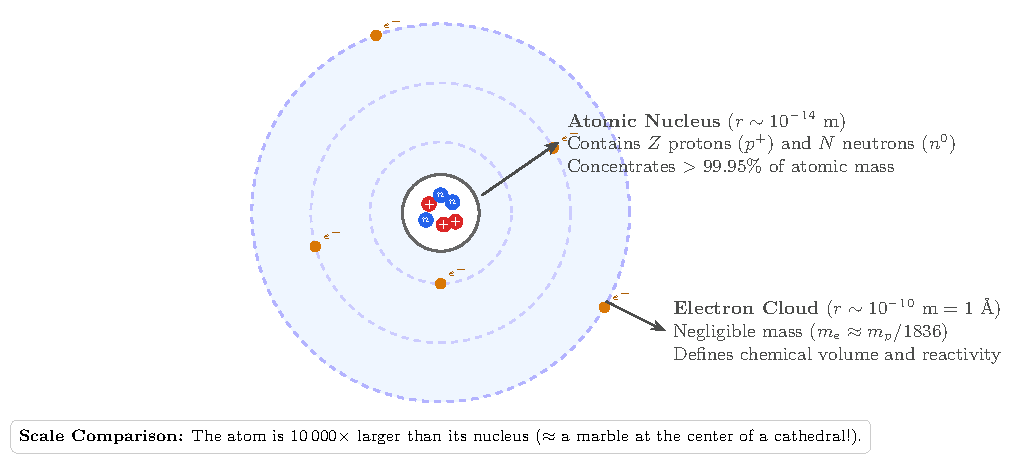
\includegraphics[width=0.74\textwidth]{figures/04_atom_structure.pdf}
\caption{The internal anatomy of the atom. The dense, central nucleus ($r_n \sim 10^{-14}\ \mathrm{m}$) concentrates over $99.95\%$ of total atomic mass, while the surrounding electron cloud ($r_{\text{atom}} \sim 10^{-10}\ \mathrm{m}$) governs atomic volume and chemical bonding.}
\label{fig:atom_structure}
\end{figure}

\subsection{1. Historical Discoveries of Subatomic Particles}
\begin{itemize}[leftmargin=1.5em,itemsep=4pt]
  \item \textbf{The Electron ($e^-$):} Discovered in 1897 by British physicist Joseph John Thomson at the Cavendish Laboratory using cathode ray tubes. By subjecting cathode ray beams to crossed electric and magnetic fields, Thomson measured their charge-to-mass ratio ($e/m_e \approx -1.7588 \times 10^{11}\ \mathrm{C\cdot kg^{-1}}$), proving that cathode rays consist of universal, negatively charged corpuscles possessing less than $1/1800$ the mass of a hydrogen atom.
  \item \textbf{The Proton ($p^+$):} Following his 1911 gold foil scattering experiment which revealed that positive charge is concentrated in a tiny central nucleus, Ernest Rutherford in 1919 bombarded nitrogen gas with energetic alpha particles ($^4_2\mathrm{He}^{2+}$), detecting emitted hydrogen nuclei:
  \[
  \ce{^{14}_7N + ^4_2He -> ^{17}_8O + ^1_1p}.
  \]
  Rutherford named this fundamental positive nuclear particle the \textbf{proton}.
  \item \textbf{The Neutron ($n^0$):} In 1932, James Chadwick irradiated beryllium with alpha particles and observed an intensely penetrating, electrically neutral radiation capable of ejecting high-energy protons from paraffin wax. Chadwick proved these neutral corpuscles were elementary nucleons of mass nearly identical to the proton, completing the nuclear triad.
\end{itemize}

\begin{historicalbox}{J.~J.~Thomson, Rutherford, and Chadwick: Unlocking the Nucleus}
\begin{minipage}{0.30\textwidth}
\centering
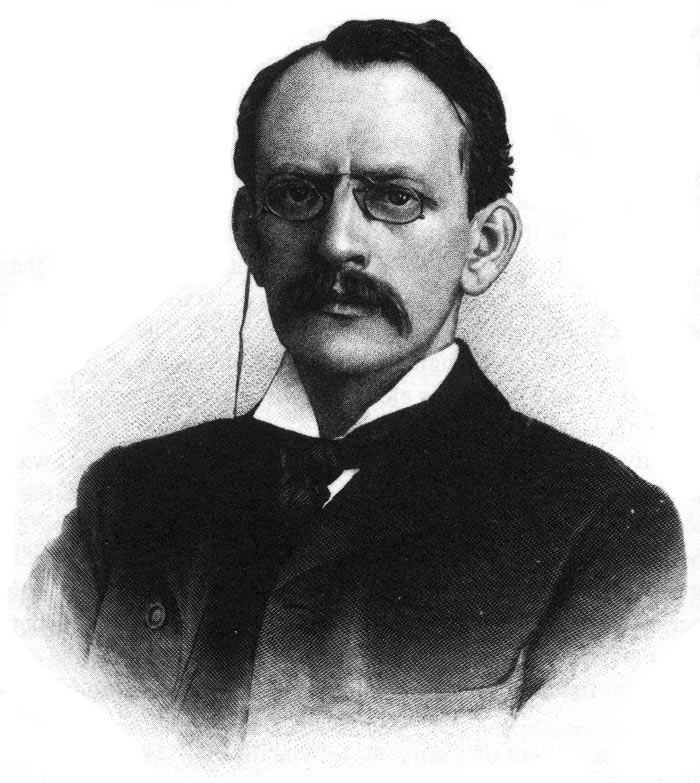
\includegraphics[width=0.92\textwidth]{images/thomson.jpg}
\captionof{figure}{J.~J.~Thomson (1856--1940).}
\end{minipage}\hfill
\begin{minipage}{0.30\textwidth}
\centering
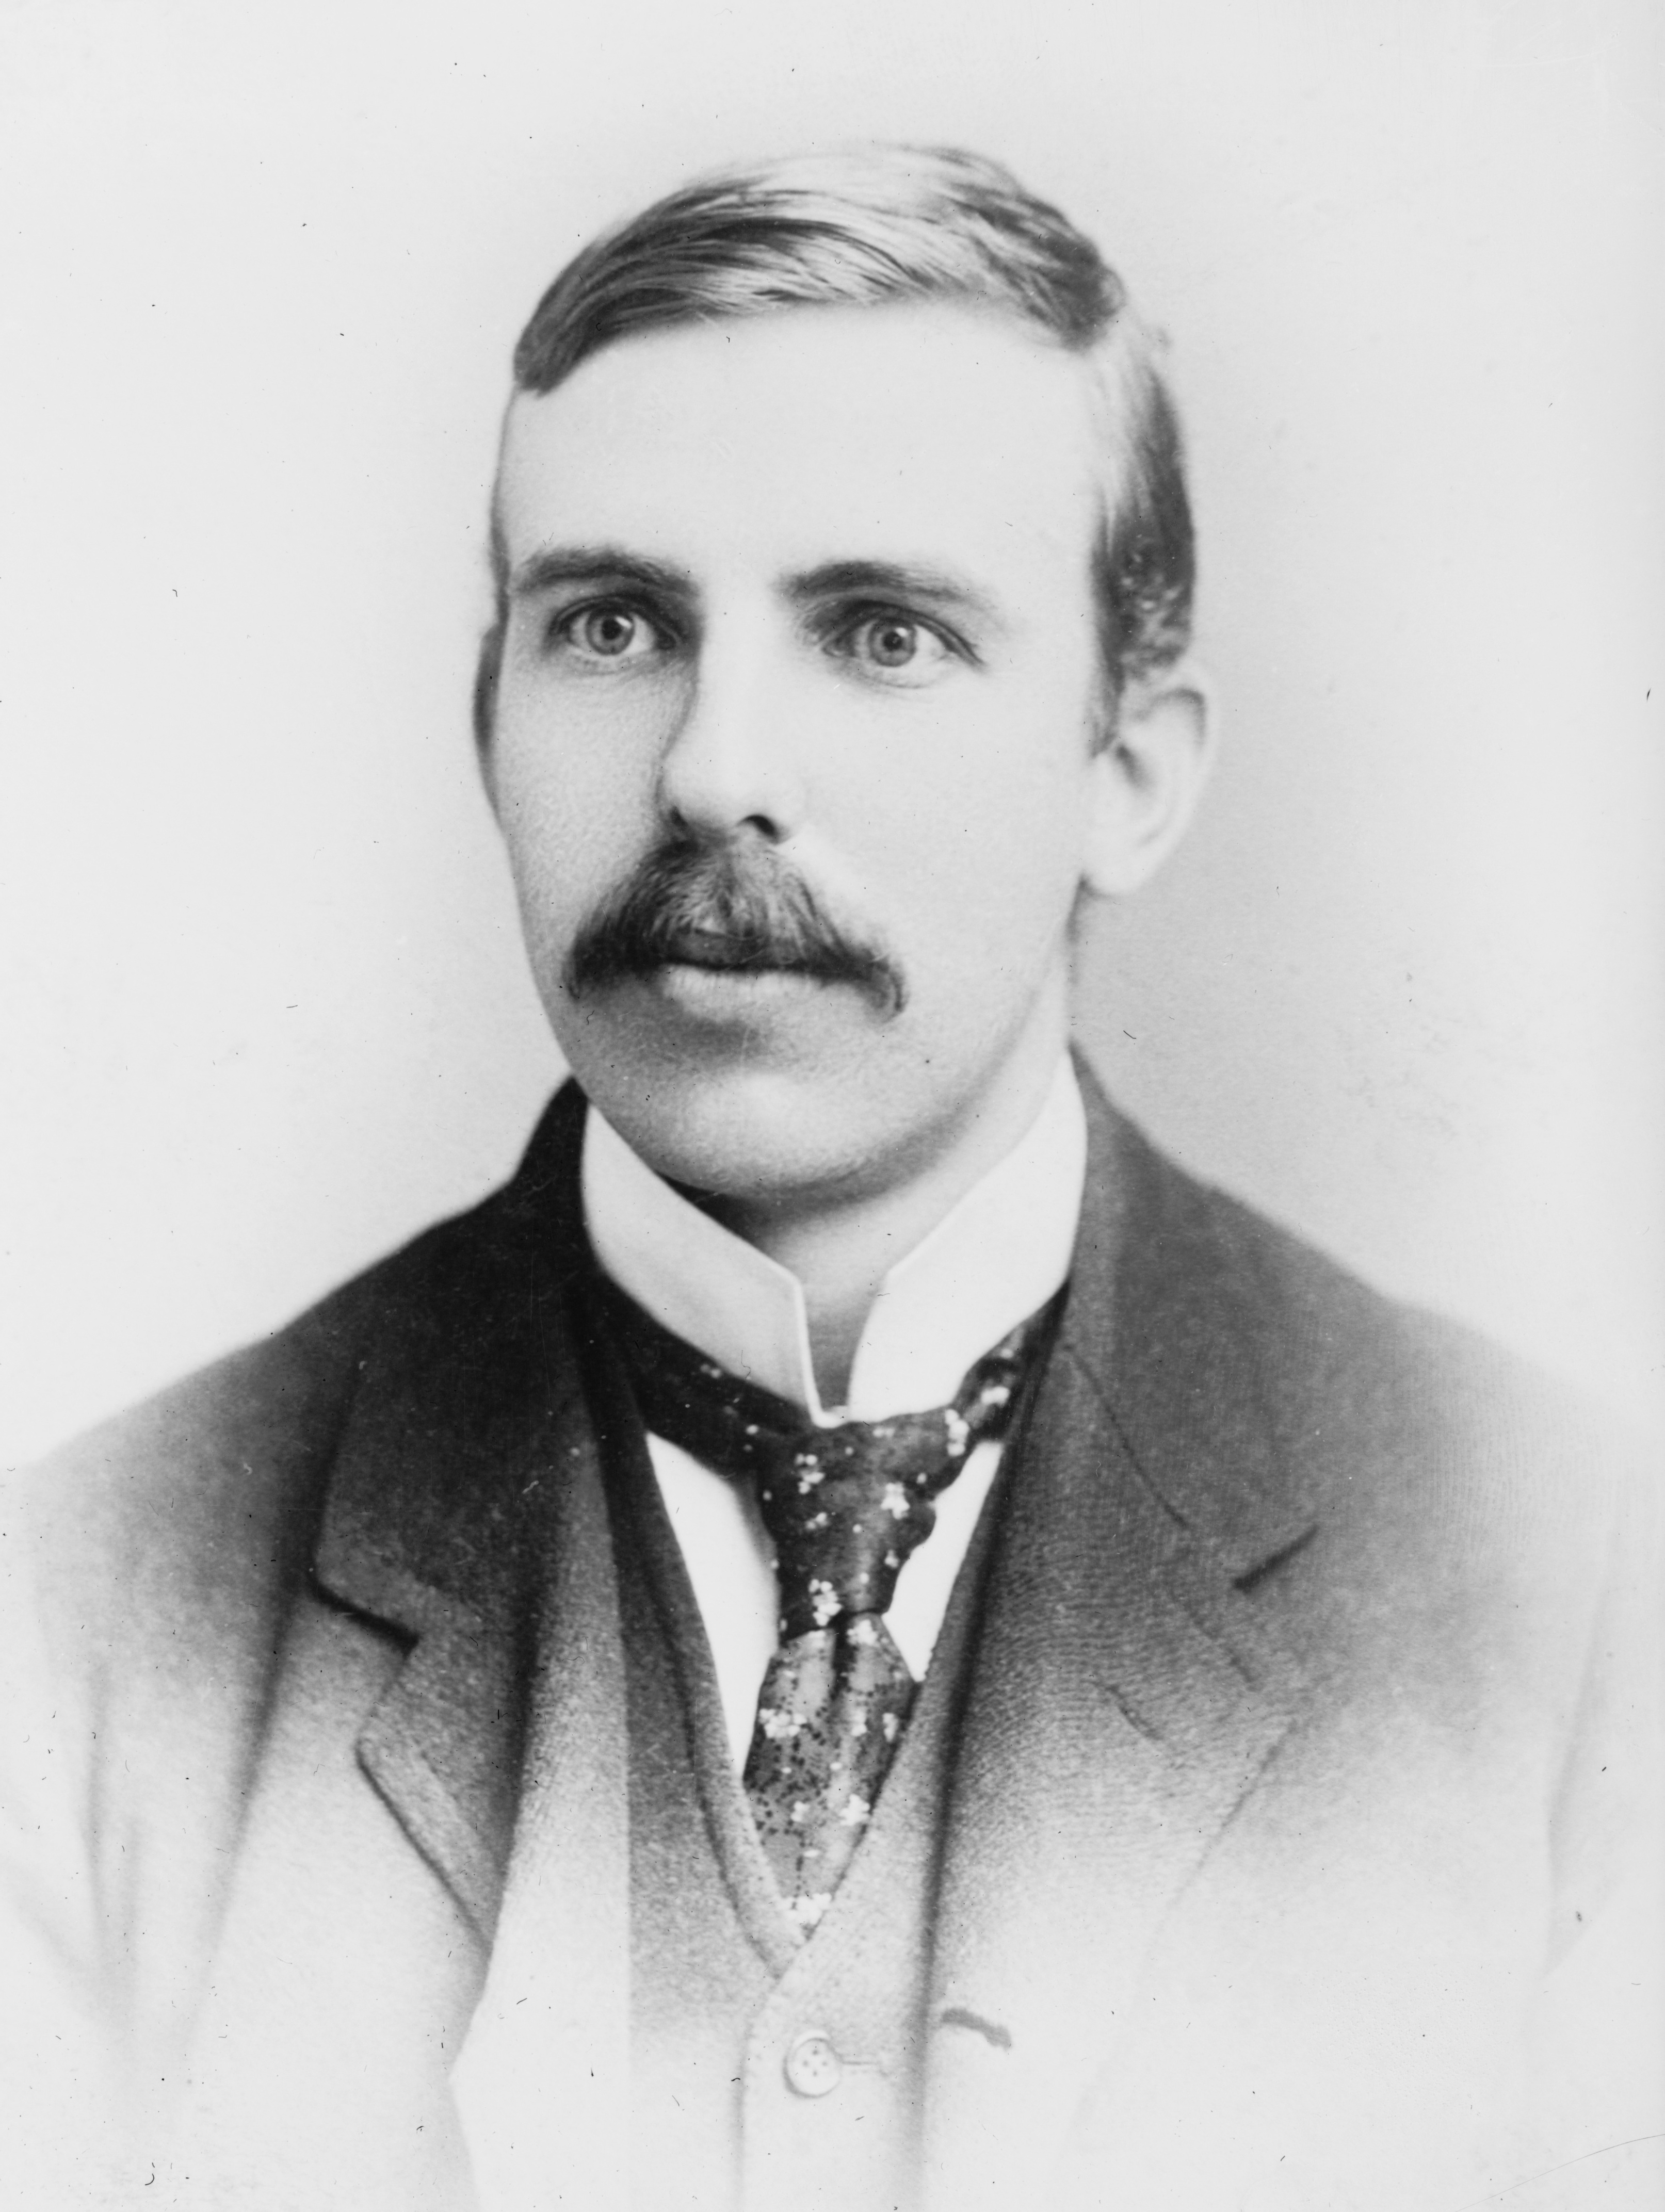
\includegraphics[width=0.92\textwidth]{images/rutherford.jpg}
\captionof{figure}{Ernest Rutherford (1871--1937).}
\end{minipage}\hfill
\begin{minipage}{0.30\textwidth}
\centering
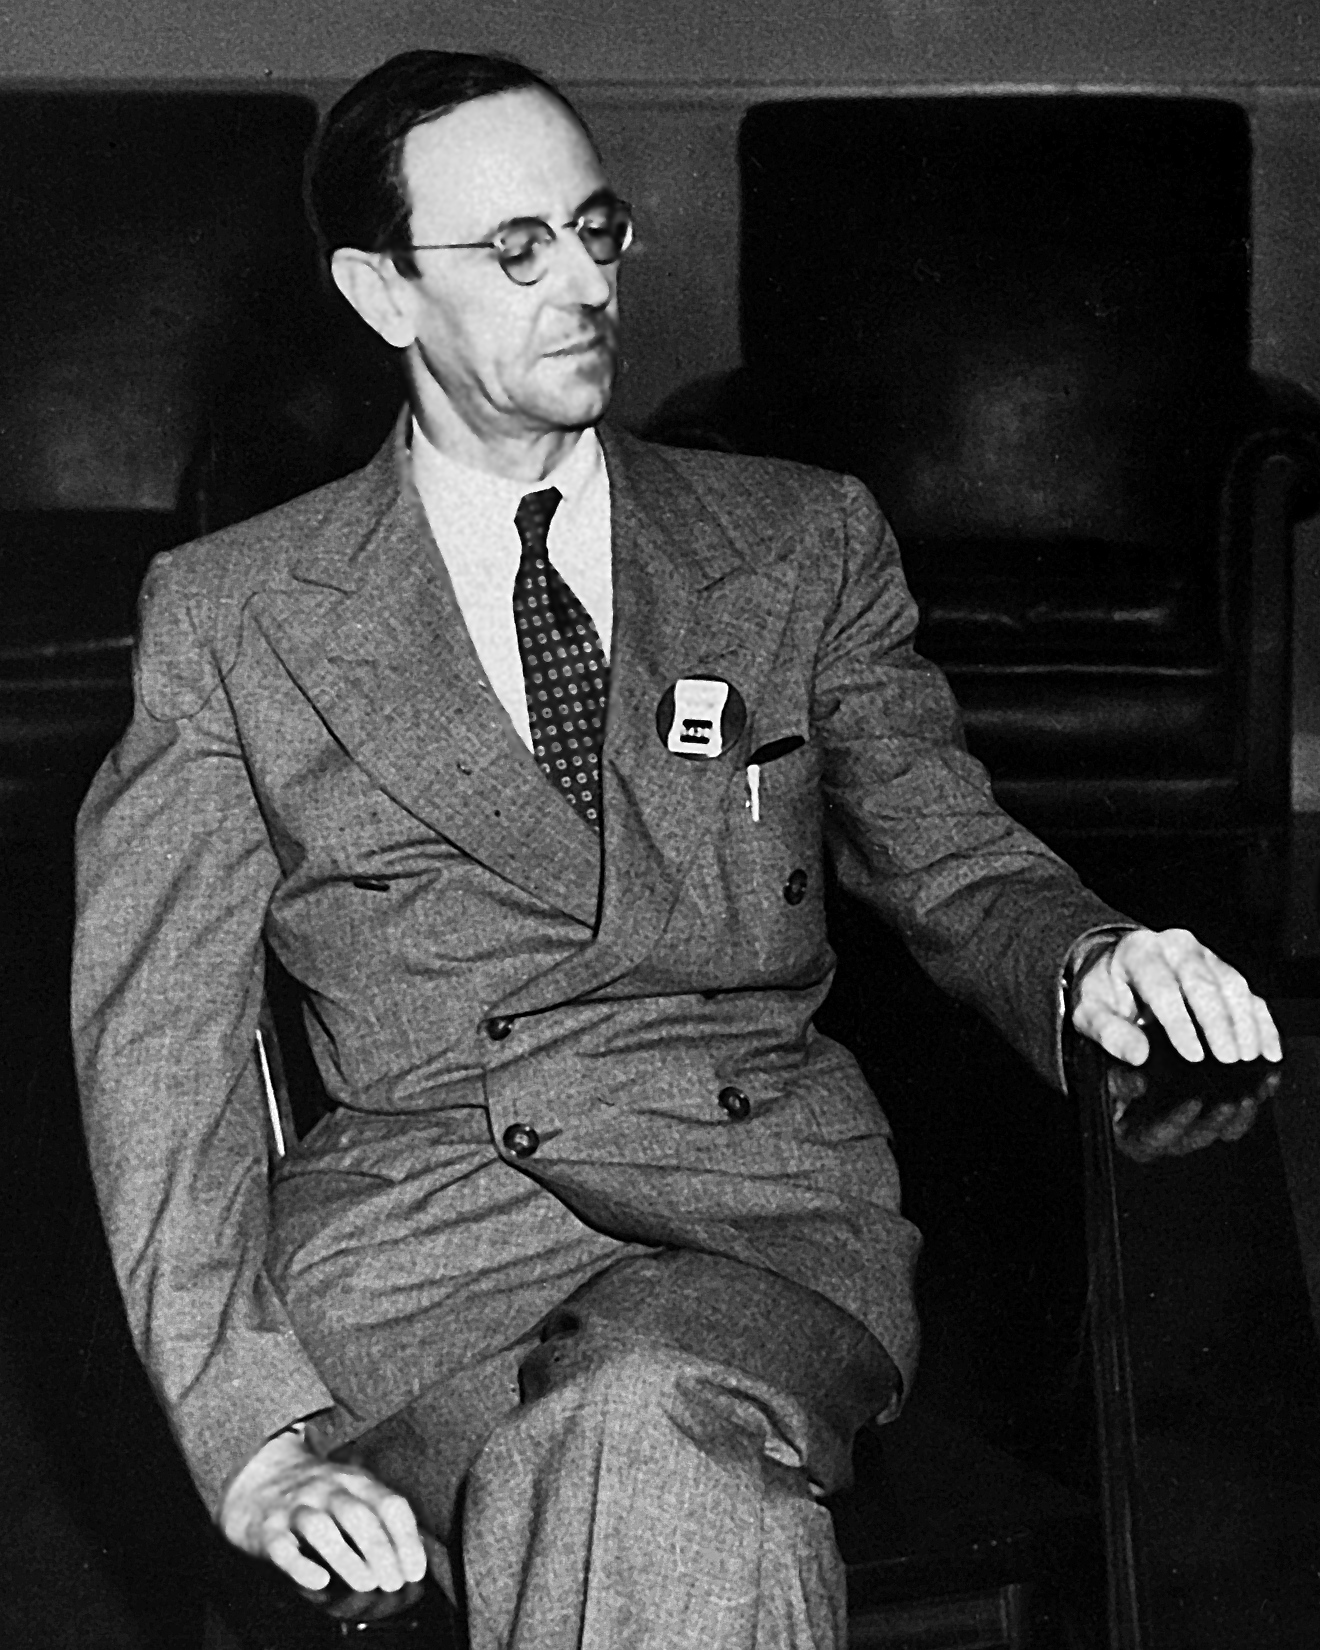
\includegraphics[width=0.92\textwidth]{images/chadwick.jpg}
\captionof{figure}{James Chadwick (1891--1974).}
\end{minipage}

Across four decades of extraordinary experimental physics at Cambridge University's Cavendish Laboratory, J.~J.~Thomson discovered the first fundamental particle (the electron, 1897); his student Ernest Rutherford discovered the atomic nucleus (1911) and the proton (1919); and Rutherford's student James Chadwick discovered the neutron (1932), establishing the modern physical model of the atom.
\end{historicalbox}

\begin{table}[htbp]
\centering
\renewcommand{\arraystretch}{1.35}
\begin{tabular}{@{}llllll@{}}
\toprule
\textbf{Particle} & \textbf{Symbol} & \textbf{Electric Charge (C)} & \textbf{Relative Charge} & \textbf{Rest Mass (kg)} & \textbf{Rest Mass (u)} \\
\midrule
\textbf{Proton} & $p$ (or $^1_1p$) & $+1.602\,176\,634 \times 10^{-19}$ & $+1$ & $1.672\,622 \times 10^{-27}$ & $1.007\,276\ \mathrm{u}$ \\
\textbf{Neutron} & $n$ (or $^1_0n$) & $0$ & $0$ & $1.674\,927 \times 10^{-27}$ & $1.008\,665\ \mathrm{u}$ \\
\textbf{Electron} & $e^-$ (or $^0_{-1}e$) & $-1.602\,176\,634 \times 10^{-19}$ & $-1$ & $9.109\,384 \times 10^{-31}$ & $0.000\,549\ \mathrm{u}$ \\
\bottomrule
\end{tabular}
\caption{Fundamental physical constants of the three subatomic constituents of matter.}
\label{tab:subatomic_particles}
\end{table}

\section{Nuclide Representation and Electronic Accounting}

\begin{definitionbox}{Standard Symbolic Representation of a Nuclide}
A specific nuclear species (a \textbf{nuclide}) of chemical element $\mathrm{X}$ is designated by the standardized IUPAC notation:
\begin{equation}
\ce{^{A}_{Z}X^{\pm q}},
\end{equation}
where:
\begin{itemize}[leftmargin=1.5em,itemsep=3pt]
  \item $Z$ is the \textbf{atomic number} (or \emph{charge number}), denoting the exact number of protons in the nucleus. It uniquely establishes the chemical identity and placement of the element in the periodic table.
  \item $A$ is the \textbf{mass number}, denoting the total integer count of nucleons (protons plus neutrons) in the nucleus:
  \begin{equation}
  A = Z + N.
  \end{equation}
  \item $N = A - Z$ is the number of neutrons.
  \item $\pm q$ is the net ionic charge (in units of elementary charge $e$).
\end{itemize}
\end{definitionbox}

\begin{lawbox}{Electronic Accounting in Atoms and Ions}
For any nuclide species $\ce{^{A}_{Z}X^{\pm q}}$:
\begin{enumerate}[leftmargin=1.5em,itemsep=3pt]
  \item \textbf{Electrically Neutral Atom ($q = 0$):} The positive nuclear charge is balanced by an identical number of surrounding orbital electrons:
  \begin{equation}
  N_{e^-} = Z.
  \end{equation}
  \item \textbf{Cation ($\ce{X^{q+}}$ with $q > 0$):} Formed when an atom loses $q$ valence electrons. The electron count is reduced:
  \begin{equation}
  N_{e^-} = Z - q.
  \end{equation}
  \item \textbf{Anion ($\ce{X^{q-}}$ with $q > 0$):} Formed when an atom gains $q$ additional electrons. The electron count is increased:
  \begin{equation}
  N_{e^-} = Z + q.
  \end{equation}
\end{enumerate}
\end{lawbox}

\section{Isotopes, Mass Spectrometry, and Relative Atomic Mass}

\subsection{Definition of Isotopes}
\begin{definitionbox}{Isotopes}
\textbf{Isotopes} are nuclides of the same chemical element that possess the **same atomic number $Z$** (identical proton and electron counts, hence identical chemical reactivity), but **different mass numbers $A$** (different numbers of neutrons $N$).
\end{definitionbox}

Because isotopes share identical chemical properties, they cannot be separated by standard chemical reactions; separation requires physical mass-dependent techniques such as **mass spectrometry**, gaseous diffusion, or ultracentrifugation.

\begin{historicalbox}{Francis William Aston and the Mass Spectrograph}
\begin{minipage}{0.28\textwidth}
\centering
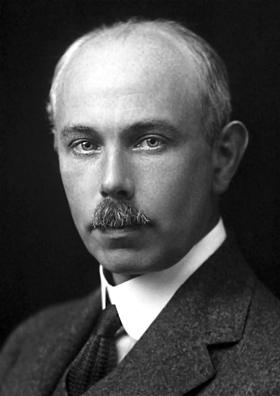
\includegraphics[width=0.92\textwidth]{images/aston.jpg}
\captionof{figure}{Francis William Aston (1877--1945), Nobel Prize in Chemistry 1922.}
\end{minipage}\hfill
\begin{minipage}{0.68\textwidth}
Working at the Cavendish Laboratory, British chemist and physicist Francis William Aston invented the electromagnetic **mass spectrograph** in 1919. By ionizing gas atoms and passing them through coordinated electric and magnetic fields, Aston focused ions of differing mass-to-charge ratios ($m/q$) onto distinct photographic lines.

Aston discovered 212 of the 287 naturally occurring stable isotopes, proving that non-integer elemental atomic weights (such as chlorine at $35.45\ \mathrm{u}$) arise naturally from weighted statistical mixtures of integer-mass isotopes ($^{35}\mathrm{Cl}$ and $^{37}\mathrm{Cl}$), formulating the **Whole Number Rule**.
\end{minipage}
\end{historicalbox}

\subsection{Canonical Isotopic Families}
\begin{itemize}[leftmargin=1.5em,itemsep=3pt]
  \item \textbf{Hydrogen Isotopes:}
  \begin{itemize}[leftmargin=1.2em]
    \item \textbf{Protium} ($\ce{^1_1H}$): $1\ p^+, 0\ n^0, 1\ e^-$ ($99.985\%$ natural terrestrial abundance).
    \item \textbf{Deuterium} ($\ce{^2_1H}$ or $\mathrm{D}$): $1\ p^+, 1\ n^0, 1\ e^-$ ($0.015\%$, stable; forms heavy water $\mathrm{D_2O}$).
    \item \textbf{Tritium} ($\ce{^3_1H}$ or $\mathrm{T}$): $1\ p^+, 2\ n^0, 1\ e^-$ (unstable, radioactive beta emitter, $t_{1/2} = 12.32\ \mathrm{yr}$).
  \end{itemize}
  \item \textbf{Carbon Isotopes:}
  \begin{itemize}[leftmargin=1.2em]
    \item $\ce{^{12}_6C}$: $6\ p^+, 6\ n^0$ ($98.93\%$ natural abundance; SI atomic mass definition standard).
    \item $\ce{^{13}_6C}$: $6\ p^+, 7\ n^0$ ($1.07\%$ natural abundance; nonzero nuclear spin $I = 1/2$, active in NMR spectroscopy).
    \item $\ce{^{14}_6C}$: $6\ p^+, 8\ n^0$ (radioactive trace $\sim 1.2 \times 10^{-12}$, used in radiocarbon archaeological dating).
  \end{itemize}
\end{itemize}

\subsection{Relative Average Atomic Mass}
In nature, an element $\mathrm{X}$ exists as a stable mixture of $k$ isotopes, each possessing a precise rest mass $m_i$ and a fractional natural abundance $x_i \in [0, 1]$ (or percentage abundance $\alpha_i = x_i \times 100\%$):

\begin{lawbox}{Average Relative Atomic Mass Formula}
The macroscopic average atomic mass $m_a$ (and molar mass $M$) of an element is the abundance-weighted arithmetic mean over all its natural isotopes:
\begin{equation}
m_a = \sum_{i=1}^k x_i \cdot m_i = \frac{\sum_{i=1}^k \alpha_i \cdot m_i}{\sum_{i=1}^k \alpha_i} = \frac{\sum_{i=1}^k \alpha_i \cdot m_i}{100\%},
\end{equation}
where $\sum_{i=1}^k x_i \equiv 1$ and $\sum_{i=1}^k \alpha_i \equiv 100\%$.
\end{lawbox}

\section{Nuclear Cohesion, Mass Defect, and Binding Energy}

\subsection{1. The Phenomenon of Mass Defect}
When isolated, unbound nucleons (protons and neutrons) coalesce under the strong nuclear force to assemble a bound atomic nucleus, high-precision mass spectrometry reveals that **the mass of the bound nucleus $M_{\text{nucleus}}$ is strictly and measurably less than the sum of the masses of its constituent free nucleons**:
\begin{equation}
M_{\text{nucleus}} < Z \cdot m_p + (A - Z) \cdot m_n.
\end{equation}

\begin{definitionbox}{Nuclear Mass Defect ($\Delta m$)}
The \textbf{mass defect} $\Delta m$ of a nucleus $\ce{^{A}_{Z}X}$ is defined as the positive difference between the total mass of its separated free nucleons and the actual mass of the assembled bound nucleus:
\begin{equation}
\Delta m \eqdef \left[ Z \cdot m_p + (A - Z) \cdot m_n \right] - M_{\text{nucleus}} > 0.
\end{equation}
Because laboratory tables list neutral atomic masses $M_{\text{atom}}(\ce{^{A}_{Z}X})$ rather than bare nuclear masses, adding $Z$ electron masses to both terms yields the equivalent atomic formulation:
\begin{equation}
\Delta m = \left[ Z \cdot m(\ce{^1_1H}) + (A - Z) \cdot m_n \right] - M_{\text{atom}}(\ce{^{A}_{Z}X}),
\end{equation}
where $m(\ce{^1_1H}) = m_p + m_e = 1.007\,825\ \mathrm{u}$ is the mass of a neutral hydrogen atom.
\end{definitionbox}

\begin{historicalbox}{Albert Einstein and the Mass-Energy Equivalence ($E = mc^2$)}
\begin{minipage}{0.28\textwidth}
\centering
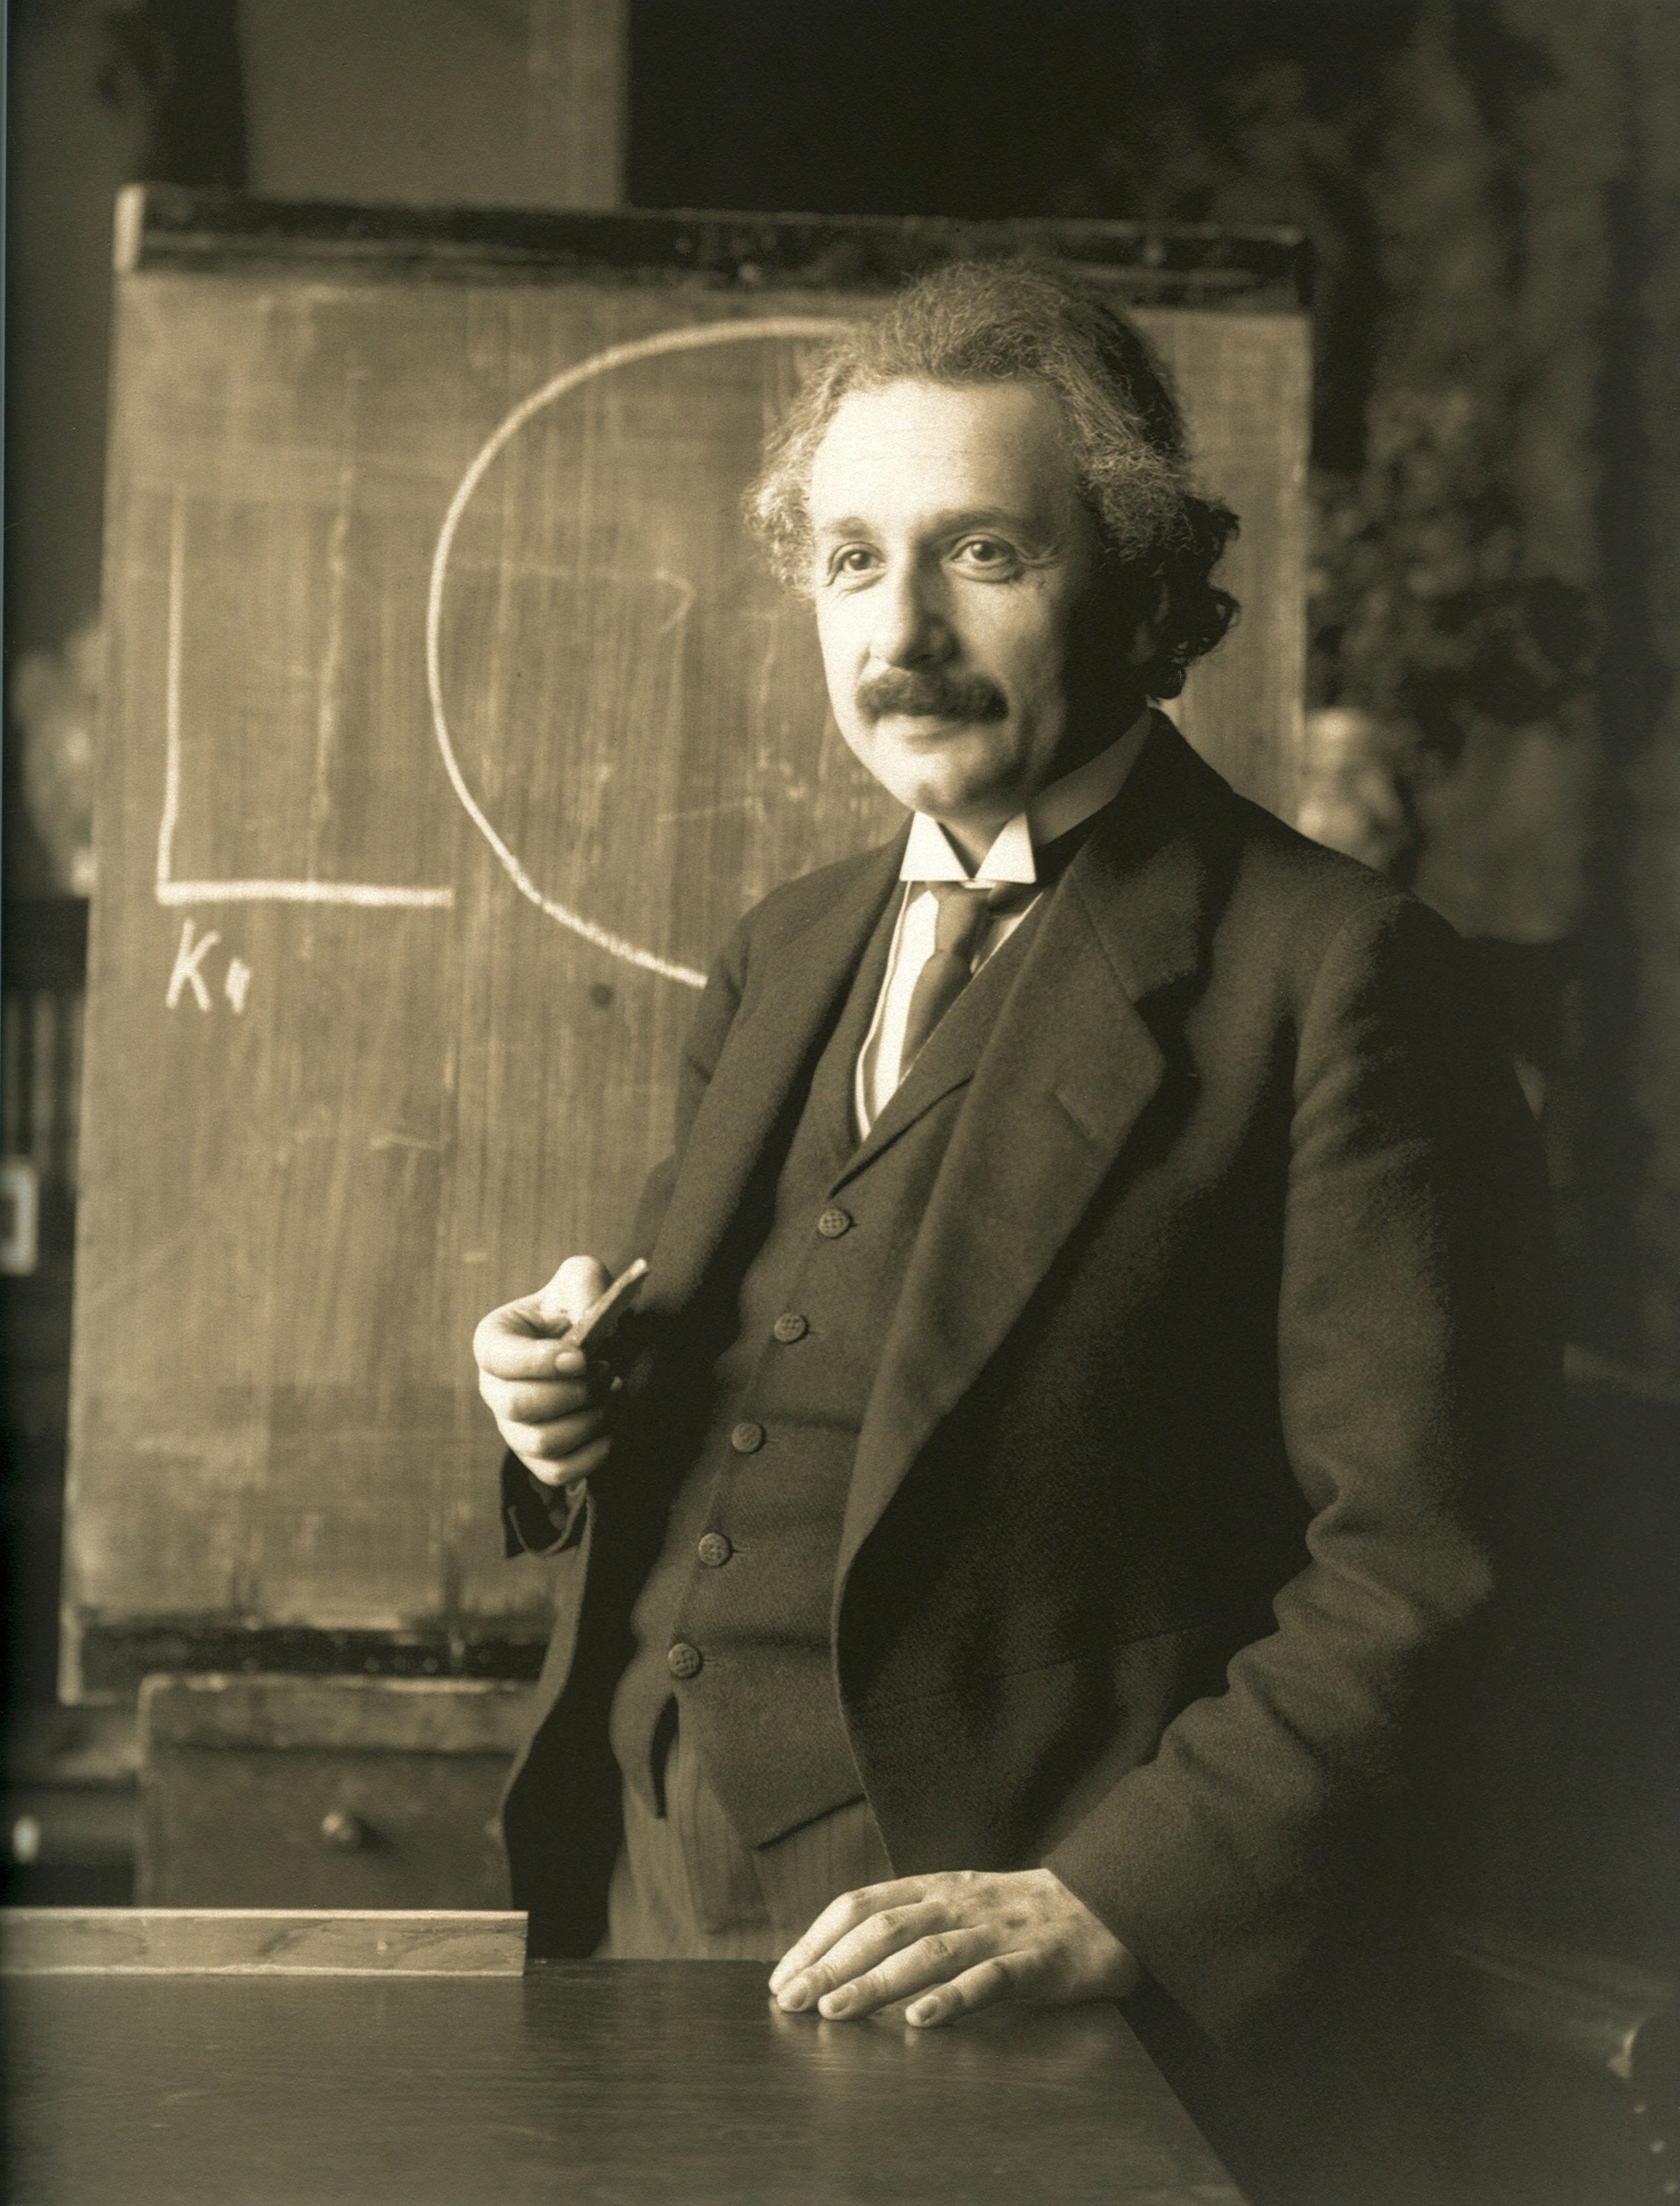
\includegraphics[width=0.92\textwidth]{images/einstein.jpg}
\captionof{figure}{Albert Einstein (1879--1955), portrait by Ferdinand Schmutzer (1921).}
\end{minipage}\hfill
\begin{minipage}{0.68\textwidth}
In September 1905, Albert Einstein published his fourth \emph{Annus Mirabilis} paper in \emph{Annalen der Physik}: ``\emph{Does the Inertia of a Body Depend upon its Energy Content?}'' 

Einstein deduced that mass is not an immutable substance, but concentrated potential energy:
\[
E = m \cdot c^2.
\]
The ``missing mass'' $\Delta m$ in atomic nuclei is converted during nuclear synthesis into binding energy, explaining why nuclear reactions release over \textbf{one million times} more energy per gram than any chemical combustion!
\end{minipage}
\end{historicalbox}

\subsection{2. Nuclear Binding Energy}

\begin{definitionbox}{Nuclear Binding Energy ($E_L$)}
The \textbf{binding energy} $E_L$ of a nucleus is defined as the minimum energy that must be supplied from the outside to dissociate the bound nucleus into its separate, non-interacting constituent nucleons at rest at infinity:
\begin{equation}
E_L \eqdef \Delta m \cdot c^2 > 0.
\end{equation}
Conversely, when free nucleons assemble to form the nucleus, an equivalent quantity of energy $\Delta E = -E_L < 0$ is released into the surroundings.
\end{definitionbox}

\subsection{3. Energy Conversion Factors}
In nuclear physics, energies are expressed in electronvolts ($\mathrm{eV}$) and mega-electronvolts ($\mathrm{MeV}$):
\begin{equation}
1\ \mathrm{eV} \eqdef 1.602\,176\,634 \times 10^{-19}\ \mathrm{J}, \qquad 1\ \mathrm{MeV} = 10^6\ \mathrm{eV} = 1.602\,176\,634 \times 10^{-13}\ \mathrm{J}.
\end{equation}
Using the speed of light in vacuum $c = 2.997\,924\,58 \times 10^8\ \mathrm{m\cdot s^{-1}}$, the energy equivalence of one atomic mass unit ($1\ \mathrm{u}$) is:
\[
E = (1.660\,539 \times 10^{-27}\ \mathrm{kg}) \times (2.997\,924\,58 \times 10^8\ \mathrm{m\cdot s^{-1}})^2 = 1.492\,418 \times 10^{-10}\ \mathrm{J}.
\]
Dividing by $1.602\,176\,634 \times 10^{-13}\ \mathrm{J/MeV}$:

\begin{lawbox}{The Universal Nuclear Conversion Constant}
\begin{equation}
1\ \mathrm{u} \cdot c^2 = \mathbf{931.494\ \mathrm{MeV}} \quad (\text{often rounded to } 931.5\ \mathrm{MeV}).
\end{equation}
Therefore, given mass defect $\Delta m$ directly in atomic mass units ($\mathrm{u}$):
\begin{equation}
E_L\ [\mathrm{MeV}] = \Delta m\ [\mathrm{u}] \times 931.494\ \mathrm{MeV\cdot u^{-1}}.
\end{equation}
\end{lawbox}

\section{Nuclear Stability and the Aston Curve}

While total binding energy $E_L$ increases monotonically with the total number of nucleons $A$, it does not measure the \emph{intrinsic stability} of a nucleus: a large nucleus like Uranium-238 has $E_L \approx 1800\ \mathrm{MeV}$, yet it is unstable and radioactively decays, while Iron-56 has $E_L \approx 492\ \mathrm{MeV}$ and is completely stable.

\begin{definitionbox}{Binding Energy per Nucleon ($E_L / A$)}
The true physical measure of nuclear cohesion and stability is the **binding energy per nucleon** (or \emph{specific binding energy}):
\begin{equation}
\frac{E_L}{A} \eqdef \frac{\Delta m \cdot c^2}{A}, \qquad \left[\frac{E_L}{A}\right] = \mathrm{MeV\cdot nucleon^{-1}}.
\end{equation}
The higher the value of $E_L / A$, the more tightly bound each nucleon is, and the more stable the atomic nucleus.
\end{definitionbox}

\begin{figure}[htbp]
\centering
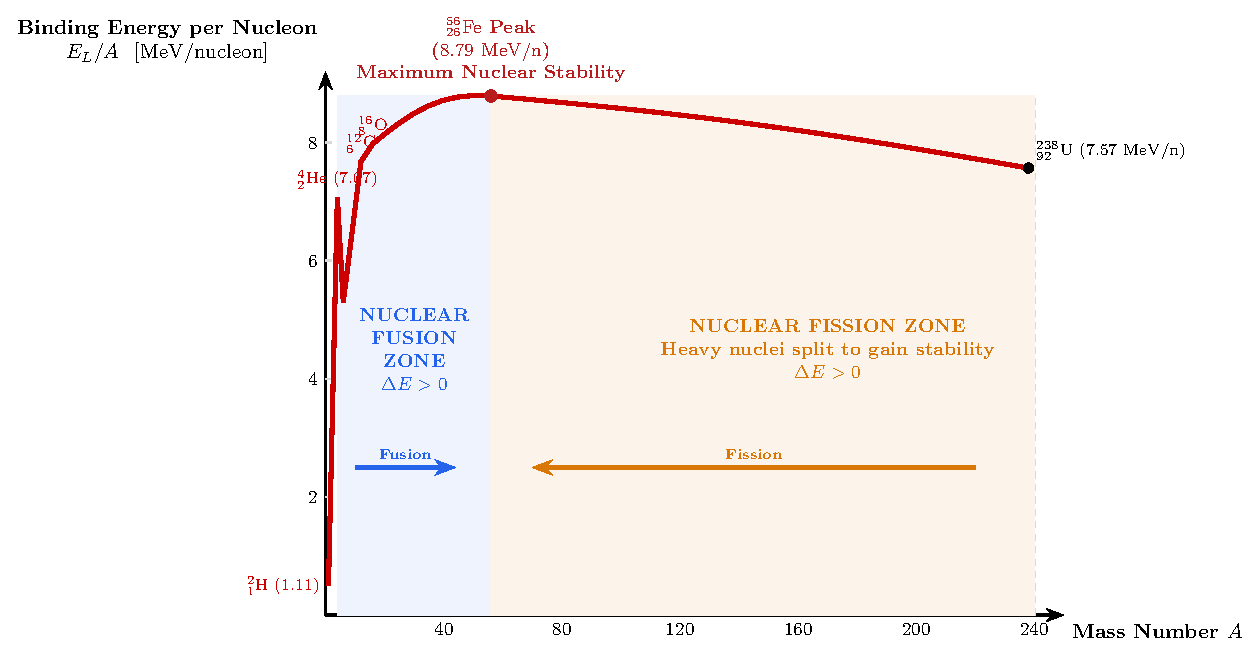
\includegraphics[width=0.88\textwidth]{figures/05_aston_curve.pdf}
\caption{The Aston Binding Energy Curve ($E_L / A$ versus mass number $A$). Nuclear stability peaks at Iron-56 ($^{56}_{26}\mathrm{Fe}$, $8.79\ \mathrm{MeV/nucleon}$). Exothermic nuclear fusion occurs for light nuclei ($A < 56$), while exothermic nuclear fission occurs for heavy nuclei ($A > 56$).}
\label{fig:aston_curve}
\end{figure}

\subsection{Thermodynamic Analysis of the Aston Curve}
The Aston curve exhibits three profound structural zones:
\begin{enumerate}[leftmargin=1.5em,itemsep=4pt]
  \item \textbf{Rapid Rise for Light Nuclei ($A < 20$):}
  The binding energy per nucleon rises steeply from $1.11\ \mathrm{MeV/n}$ in deuterium ($\ce{^2_1H}$) up to $\approx 8\ \mathrm{MeV/n}$. Pronounced local maxima occur at $\alpha$-conjugate nuclei ($\ce{^4_2He}$ at $7.07\ \mathrm{MeV/n}$, $\ce{^{12}_6C}$ at $7.68\ \mathrm{MeV/n}$, $\ce{^{16}_8O}$ at $7.98\ \mathrm{MeV/n}$), corresponding to filled nuclear energy shells.
  \item \textbf{The Iron Peak of Maximum Stability ($A \approx 56\text{--}62$):}
  The curve attains its global maximum at:
  \begin{equation}
  \left(\frac{E_L}{A}\right)_{\max} \approx 8.79\ \mathrm{MeV\cdot nucleon^{-1}} \quad \text{for } \ce{^{56}_{26}Fe} \text{ and } \ce{^{62}_{28}Ni}.
  \end{equation}
  Iron-56 and Nickel-62 are the most thermodynamically stable nuclei in the universe. They represent the final energetic endpoint of stellar nucleosynthesis in massive stars.
  \item \textbf{Gradual Decline for Heavy Nuclei ($A > 60$):}
  Beyond iron, $E_L / A$ gradually drops to $7.57\ \mathrm{MeV/n}$ for Uranium-238 ($\ce{^{238}_{92}U}$). This decrease is driven by the long-range electrostatic Coulomb repulsion between protons ($V_C \propto Z^2/R$), which scales faster than the short-range strong nuclear attraction.
\end{enumerate}

\begin{lawbox}{Thermodynamics of Nuclear Energy: Fusion vs. Fission}
Any nuclear transformation that moves a system toward the Iron Peak ($\ce{^{56}Fe}$) increases binding energy per nucleon and is **strongly exothermic** ($\Delta E_{\text{reaction}} > 0$):
\begin{itemize}[leftmargin=1.5em,itemsep=3pt]
  \item \textbf{Thermonuclear Fusion ($A \ll 56$):} Combining two light nuclei with low $E_L / A$ into a heavier nucleus with higher $E_L / A$ releases enormous energy:
  \[
  \ce{^2_1H + ^3_1H -> ^4_2He + ^1_0n} + 17.59\ \mathrm{MeV}.
  \]
  \item \textbf{Nuclear Fission ($A \gg 56$):} Splitting a massive nucleus with lower $E_L / A$ into two intermediate nuclei with higher $E_L / A$ releases energy:
  \[
  \ce{^{235}_{92}U + ^1_0n -> ^{141}_{56}Ba + ^{92}_{36}Kr + 3\,^1_0n} + 200\ \mathrm{MeV}.
  \]
\end{itemize}
\end{lawbox}

\section{Comprehensive Worked Examples}

\begin{workedexample}{Subatomic Accounting of Neutral Atoms and Complex Ions}
Determine the number of protons ($p^+$), neutrons ($n^0$), and electrons ($e^-$), as well as the total nuclear charge $Q_{\text{nucleus}}$ and electronic cloud charge $Q_{\text{electrons}}$ for each of the following chemical species:
\begin{enumerate}[leftmargin=1.4em,itemsep=2pt]
  \item Neutral Iron-56 atom: $\ce{^{56}_{26}Fe}$,
  \item Ferric iron cation: $\ce{^{56}_{26}Fe^{3+}}$,
  \item Chloride anion: $\ce{^{35}_{17}Cl^-}$,
  \item Ammonium polyatomic cation: $\ce{^{14}_7N^1_1H_4^+}$,
  \item Phosphate polyatomic anion: $\ce{^{31}_{15}P^{16}_8O_4^{3-}}$.
\end{enumerate}

\paragraph{Solution.}
Using the rules: $Z = N_{p^+}$, $N = A - Z$, $N_{e^-} = Z - q$ (for charge $+q$) and $N_{e^-} = Z + q$ (for charge $-q$).
Elementary charge is $e = 1.602 \times 10^{-19}\ \mathrm{C}$.

\textbf{1. Neutral Iron-56 ($\ce{^{56}_{26}Fe}$):}\\
$Z = 26$, $A = 56$, $q = 0$.
\begin{itemize}[leftmargin=1.5em,itemsep=1pt]
  \item Protons: $N_{p^+} = Z = \mathbf{26}$.
  \item Neutrons: $N_{n^0} = A - Z = 56 - 26 = \mathbf{30}$.
  \item Electrons: $N_{e^-} = Z = \mathbf{26}$.
  \item $Q_{\text{nucleus}} = +26\,e = +4.165 \times 10^{-18}\ \mathrm{C}$; $Q_{\text{electrons}} = -26\,e = -4.165 \times 10^{-18}\ \mathrm{C}$ ($Q_{\text{net}} = 0$).
\end{itemize}

\textbf{2. Ferric Cation ($\ce{^{56}_{26}Fe^{3+}}$):}\\
$Z = 26$, $A = 56$, $q = +3$.
\begin{itemize}[leftmargin=1.5em,itemsep=1pt]
  \item Protons: $N_{p^+} = Z = \mathbf{26}$.
  \item Neutrons: $N_{n^0} = 56 - 26 = \mathbf{30}$.
  \item Electrons: $N_{e^-} = Z - 3 = 26 - 3 = \mathbf{23}$.
  \item Net charge: $Q_{\text{net}} = +3\,e = +4.806 \times 10^{-19}\ \mathrm{C}$.
\end{itemize}

\textbf{3. Chloride Anion ($\ce{^{35}_{17}Cl^-}$):}\\
$Z = 17$, $A = 35$, $q = -1$.
\begin{itemize}[leftmargin=1.5em,itemsep=1pt]
  \item Protons: $N_{p^+} = Z = \mathbf{17}$.
  \item Neutrons: $N_{n^0} = 35 - 17 = \mathbf{18}$.
  \item Electrons: $N_{e^-} = Z + 1 = 17 + 1 = \mathbf{18}$ (argon noble-gas configuration).
  \item Net charge: $Q_{\text{net}} = -1\,e = -1.602 \times 10^{-19}\ \mathrm{C}$.
\end{itemize}

\textbf{4. Ammonium Polyatomic Cation ($\ce{NH_4^+}$):}\\
Consists of one Nitrogen ($\ce{^{14}_7N}$) and four Hydrogens ($\ce{^1_1H}$), net charge $q = +1$.
\begin{itemize}[leftmargin=1.5em,itemsep=1pt]
  \item Total protons: $N_{p^+} = Z(\mathrm{N}) + 4 \times Z(\mathrm{H}) = 7 + 4(1) = \mathbf{11}$.
  \item Total neutrons: $N_{n^0} = (14 - 7) + 4 \times (1 - 1) = 7 + 0 = \mathbf{7}$.
  \item Total electrons: $N_{e^-} = N_{p^+} - 1 = 11 - 1 = \mathbf{10}$ (neon configuration).
\end{itemize}

\textbf{5. Phosphate Polyatomic Anion ($\ce{PO_4^{3-}}$):}\\
Consists of one Phosphorus ($\ce{^{31}_{15}P}$) and four Oxygens ($\ce{^{16}_8O}$), net charge $q = -3$.
\begin{itemize}[leftmargin=1.5em,itemsep=1pt]
  \item Total protons: $N_{p^+} = Z(\mathrm{P}) + 4 \times Z(\mathrm{O}) = 15 + 4(8) = 15 + 32 = \mathbf{47}$.
  \item Total neutrons: $N_{n^0} = (31 - 15) + 4 \times (16 - 8) = 16 + 4(8) = 16 + 32 = \mathbf{48}$.
  \item Total electrons: $N_{e^-} = N_{p^+} + 3 = 47 + 3 = \mathbf{50}$.
\end{itemize}
\end{workedexample}

\begin{workedexample}{Determination of Isotopic Abundances from Mass Spectrometry}
Natural copper ($\mathrm{Cu}$) consists of two stable isotopes: $\ce{^{63}_{29}Cu}$ and $\ce{^{65}_{29}Cu}$. High-resolution mass spectrometry gives their isotopic rest masses:
\[
m(\ce{^{63}Cu}) = 62.9296\ \mathrm{u}, \qquad m(\ce{^{65}Cu}) = 64.9278\ \mathrm{u}.
\]
The standard relative atomic mass of naturally occurring copper is $M(\mathrm{Cu}) = 63.5460\ \mathrm{u}$.
\begin{enumerate}[leftmargin=1.4em,itemsep=3pt]
  \item Calculate the fractional abundances ($x_1, x_2$) and percentage abundances ($\alpha_1, \alpha_2$) of the two isotopes in nature.
  \item For a pure foil of copper weighing $m_{\text{sample}} = 10.00\ \mathrm{g}$, calculate the total number of copper atoms, and the individual number of $\ce{^{63}Cu}$ and $\ce{^{65}Cu}$ atoms present.
\end{enumerate}

\paragraph{Solution.}
\textbf{1. Isotopic Abundance System of Equations:}\\
Let $x_1$ be the fractional abundance of $\ce{^{63}Cu}$ and $x_2$ be the fractional abundance of $\ce{^{65}Cu}$.
They satisfy the system of linear equations:
\[
\begin{cases}
x_1 + x_2 = 1 \implies x_2 = 1 - x_1, \\
x_1 \cdot m_1 + x_2 \cdot m_2 = M(\mathrm{Cu}).
\end{cases}
\]
Substituting $x_2 = 1 - x_1$:
\[
x_1 \cdot m_1 + (1 - x_1) \cdot m_2 = M(\mathrm{Cu}) \implies x_1(m_1 - m_2) + m_2 = M(\mathrm{Cu}).
\]
Solving for $x_1$:
\[
x_1 = \frac{m_2 - M(\mathrm{Cu})}{m_2 - m_1} = \frac{64.9278 - 63.5460}{64.9278 - 62.9296} = \frac{1.3818}{1.9982} \approx \mathbf{0.69152} = \mathbf{69.15\%}.
\]
Then $x_2$ is:
\[
x_2 = 1 - x_1 = 1 - 0.69152 = \mathbf{0.30848} = \mathbf{30.85\%}.
\]
Natural copper is composed of $69.15\%$ Copper-63 and $30.85\%$ Copper-65.

\textbf{2. Number of Atoms in the Sample:}\\
The amount of copper in $10.00\ \mathrm{g}$ is:
\[
n = \frac{m_{\text{sample}}}{M} = \frac{10.00\ \mathrm{g}}{63.5460\ \mathrm{g\cdot mol^{-1}}} \approx 0.15737\ \mathrm{mol}.
\]
The total number of copper atoms is:
\[
N_{\text{total}} = n \cdot N_A = 0.15737\ \mathrm{mol} \times 6.02214 \times 10^{23}\ \mathrm{mol^{-1}} \approx \mathbf{9.477 \times 10^{22}\ \text{atoms}}.
\]
The number of $\ce{^{63}Cu}$ atoms is:
\[
N(\ce{^{63}Cu}) = x_1 \cdot N_{\text{total}} = 0.69152 \times 9.477 \times 10^{22} \approx \mathbf{6.554 \times 10^{22}\ \text{atoms}}.
\]
The number of $\ce{^{65}Cu}$ atoms is:
\[
N(\ce{^{65}Cu}) = x_2 \cdot N_{\text{total}} = 0.30848 \times 9.477 \times 10^{22} \approx \mathbf{2.923 \times 10^{22}\ \text{atoms}}.
\]
\end{workedexample}

\begin{workedexample}{Nuclear Mass Defect and Binding Energy of Helium-4 and Iron-56}
Given the following ultra-precise rest masses:
\begin{align*}
\text{Proton mass } m_p &= 1.007\,276\ \mathrm{u}, & \text{Neutron mass } m_n &= 1.008\,665\ \mathrm{u}, \\
\text{Hydrogen atom } m(\ce{^1_1H}) &= 1.007\,825\ \mathrm{u}, & \text{Helium-4 atom } M(\ce{^4_2He}) &= 4.002\,603\ \mathrm{u}, \\
\text{Iron-56 atom } M(\ce{^{56}_{26}Fe}) &= 55.934\,937\ \mathrm{u}.
\end{align*}
\begin{enumerate}[leftmargin=1.4em,itemsep=3pt]
  \item Calculate the mass defect $\Delta m$ of Helium-4 in $\mathrm{u}$ and in kilograms ($\mathrm{kg}$).
  \item Compute the total binding energy $E_L$ of Helium-4 in $\mathrm{MeV}$ and in joules ($\mathrm{J}$), and find its binding energy per nucleon $E_L / A$.
  \item Calculate the mass defect $\Delta m$, total binding energy $E_L$, and specific binding energy $E_L / A$ of Iron-56 ($\ce{^{56}_{26}Fe}$).
  \item Compare the stability of Helium-4 and Iron-56.
\end{enumerate}

\paragraph{Solution.}
\textbf{1. Mass Defect of Helium-4 ($\ce{^4_2He}$):}\\
A neutral $\ce{^4_2He}$ atom consists of $Z = 2$ protons, $N = A - Z = 4 - 2 = 2$ neutrons, and $2$ electrons.
Using the neutral hydrogen atom formula:
\[
\Delta m(\ce{^4He}) = \left[ 2 \cdot m(\ce{^1H}) + 2 \cdot m_n \right] - M(\ce{^4He}).
\]
\[
\Delta m = \left[ 2(1.007\,825) + 2(1.008\,665) \right] - 4.002\,603 = [2.015\,650 + 2.017\,330] - 4.002\,603.
\]
\[
\Delta m = 4.032\,980 - 4.002\,603 = \mathbf{0.030\,377\ \mathrm{u}}.
\]
In kilograms:
\[
\Delta m = 0.030\,377\ \mathrm{u} \times 1.660\,539 \times 10^{-27}\ \mathrm{kg\cdot u^{-1}} \approx \mathbf{5.0442 \times 10^{-29}\ \mathrm{kg}}.
\]

\textbf{2. Binding Energy of Helium-4:}\\
Using the conversion factor $1\ \mathrm{u} \equiv 931.494\ \mathrm{MeV}$:
\[
E_L(\ce{^4He}) = 0.030\,377\ \mathrm{u} \times 931.494\ \mathrm{MeV\cdot u^{-1}} \approx \mathbf{28.296\ \mathrm{MeV}}.
\]
In joules:
\[
E_L = 28.296 \times 10^6\ \mathrm{eV} \times 1.602\,177 \times 10^{-19}\ \mathrm{J\cdot eV^{-1}} \approx \mathbf{4.533 \times 10^{-12}\ \mathrm{J}}.
\]
The binding energy per nucleon is ($A = 4$):
\[
\frac{E_L}{A} = \frac{28.296\ \mathrm{MeV}}{4} \approx \mathbf{7.074\ \mathrm{MeV\cdot nucleon^{-1}}}.
\]

\textbf{3. Binding Energy of Iron-56 ($\ce{^{56}_{26}Fe}$):}\\
For Iron-56 ($Z = 26$, $N = 56 - 26 = 30$):
\[
\Delta m(\ce{^{56}Fe}) = \left[ 26 \cdot m(\ce{^1H}) + 30 \cdot m_n \right] - M(\ce{^{56}Fe}).
\]
\[
26 \times 1.007\,825 = 26.203\,450\ \mathrm{u}, \qquad 30 \times 1.008\,665 = 30.259\,950\ \mathrm{u}.
\]
Total mass of separated nucleons:
\[
\sum m_{\text{nucleons}} = 26.203\,450 + 30.259\,950 = 56.463\,400\ \mathrm{u}.
\]
The mass defect is:
\[
\Delta m(\ce{^{56}Fe}) = 56.463\,400 - 55.934\,937 = \mathbf{0.528\,463\ \mathrm{u}}.
\]
In kilograms: $\Delta m = 0.528\,463 \times 1.6605 \times 10^{-27} \approx 8.775 \times 10^{-28}\ \mathrm{kg}$.
The total binding energy is:
\[
E_L(\ce{^{56}Fe}) = 0.528\,463\ \mathrm{u} \times 931.494\ \mathrm{MeV\cdot u^{-1}} \approx \mathbf{492.265\ \mathrm{MeV}}.
\]
The binding energy per nucleon is ($A = 56$):
\[
\frac{E_L}{A} = \frac{492.265\ \mathrm{MeV}}{56} \approx \mathbf{8.790\ \mathrm{MeV\cdot nucleon^{-1}}}.
\]

\textbf{4. Stability Comparison:}\\
Because $\frac{E_L}{A}(\ce{^{56}Fe}) = 8.79\ \mathrm{MeV/n} > \frac{E_L}{A}(\ce{^4He}) = 7.07\ \mathrm{MeV/n}$, the nucleons in Iron-56 are substantially more tightly bound than those in Helium-4. Iron-56 represents the pinnacle of nuclear stability.
\end{workedexample}

\begin{workedexample}{Energetics of Induced Nuclear Fission vs. Thermonuclear Fusion}
Compare the energy yields of nuclear fission and fusion:
\begin{enumerate}[leftmargin=1.4em,itemsep=3pt]
  \item Consider the thermal neutron-induced fission of Uranium-235:
  \[
  \ce{^{235}_{92}U + ^1_0n -> ^{141}_{56}Ba + ^{92}_{36}Kr + 3\,^1_0n}.
  \]
  Given the isotopic masses:
  $m(\ce{^{235}U}) = 235.043\,929\ \mathrm{u}$, $m(\ce{^{141}Ba}) = 140.914\,411\ \mathrm{u}$, $m(\ce{^{92}Kr}) = 91.926\,156\ \mathrm{u}$, and $m_n = 1.008\,665\ \mathrm{u}$.
  Calculate the mass variation $\Delta M$, the energy released $\Delta E$ per fission event (in $\mathrm{MeV}$ and $\mathrm{J}$), and the specific energy yield per kilogram of Uranium-235 ($\mathrm{J\cdot kg^{-1}}$).
  \item Consider the Deuterium-Tritium ($\mathrm{D}$-$\mathrm{T}$) thermonuclear fusion:
  \[
  \ce{^2_1H + ^3_1H -> ^4_2He + ^1_0n}.
  \]
  Given: $m(\ce{^2H}) = 2.014\,102\ \mathrm{u}$, $m(\ce{^3H}) = 3.016\,049\ \mathrm{u}$, $m(\ce{^4He}) = 4.002\,603\ \mathrm{u}$.
  Calculate the energy released $\Delta E$ per fusion event (in $\mathrm{MeV}$), and the specific energy yield per kilogram of $\mathrm{D}$-$\mathrm{T}$ fuel mix ($\mathrm{J\cdot kg^{-1}}$).
  \item Compare both nuclear yields to the chemical combustion of high-grade coal ($3.0 \times 10^7\ \mathrm{J\cdot kg^{-1}}$).
\end{enumerate}

\paragraph{Solution.}
\textbf{1. Fission Energetics:}\\
Initial reactant mass:
\[
M_{\text{initial}} = m(\ce{^{235}U}) + m_n = 235.043\,929 + 1.008\,665 = 236.052\,594\ \mathrm{u}.
\]
Final product mass:
\[
M_{\text{final}} = m(\ce{^{141}Ba}) + m(\ce{^{92}Kr}) + 3\,m_n = 140.914\,411 + 91.926\,156 + 3(1.008\,665) = 235.866\,562\ \mathrm{u}.
\]
Mass defect of the reaction:
\[
\Delta M_{\text{fission}} = M_{\text{initial}} - M_{\text{final}} = 236.052\,594 - 235.866\,562 = \mathbf{0.186\,032\ \mathrm{u}}.
\]
The energy released per single fission event is:
\[
\Delta E_{\text{fission}} = 0.186\,032\ \mathrm{u} \times 931.494\ \mathrm{MeV\cdot u^{-1}} \approx \mathbf{173.29\ \mathrm{MeV}}.
\]
In joules:
\[
\Delta E_{\text{fission}} = 173.29 \times 10^6 \times 1.6022 \times 10^{-19}\ \mathrm{J} \approx \mathbf{2.776 \times 10^{-11}\ \mathrm{J}}.
\]
One kilogram of pure $\ce{^{235}U}$ contains:
\[
N = \frac{1000\ \mathrm{g}}{235.04\ \mathrm{g\cdot mol^{-1}}} \times 6.022 \times 10^{23}\ \mathrm{mol^{-1}} \approx 2.562 \times 10^{24}\ \text{nuclei}.
\]
The specific energy yield of Uranium-235 fission is:
\[
\mathcal{E}_{\text{fission}} = (2.562 \times 10^{24}) \times (2.776 \times 10^{-11}\ \mathrm{J}) \approx \mathbf{7.11 \times 10^{13}\ \mathrm{J\cdot kg^{-1}} = 71.1\ \mathrm{TJ\cdot kg^{-1}}}.
\]

\textbf{2. D-T Fusion Energetics:}\\
Initial reactant mass:
\[
M_{\text{initial}} = m(\ce{^2H}) + m(\ce{^3H}) = 2.014\,102 + 3.016\,049 = 5.030\,151\ \mathrm{u}.
\]
Final product mass:
\[
M_{\text{final}} = m(\ce{^4He}) + m_n = 4.002\,603 + 1.008\,665 = 5.011\,268\ \mathrm{u}.
\]
Mass defect of fusion:
\[
\Delta M_{\text{fusion}} = 5.030\,151 - 5.011\,268 = \mathbf{0.018\,883\ \mathrm{u}}.
\]
Energy released per single fusion event:
\[
\Delta E_{\text{fusion}} = 0.018\,883\ \mathrm{u} \times 931.494\ \mathrm{MeV\cdot u^{-1}} \approx \mathbf{17.59\ \mathrm{MeV}}.
\]
In joules:
\[
\Delta E_{\text{fusion}} = 17.59 \times 10^6 \times 1.6022 \times 10^{-19}\ \mathrm{J} \approx \mathbf{2.818 \times 10^{-12}\ \mathrm{J}}.
\]
The molar mass of the stoichiometric $\mathrm{D}$-$\mathrm{T}$ reaction pair is:
\[
M_{\text{pair}} \approx 2.014 + 3.016 = 5.030\ \mathrm{g\cdot mol^{-1}}.
\]
One kilogram of $\mathrm{D}$-$\mathrm{T}$ fuel contains:
\[
N_{\text{pairs}} = \frac{1000\ \mathrm{g}}{5.030\ \mathrm{g\cdot mol^{-1}}} \times 6.022 \times 10^{23}\ \mathrm{mol^{-1}} \approx 1.197 \times 10^{26}\ \text{pairs}.
\]
The specific energy yield of $\mathrm{D}$-$\mathrm{T}$ fusion is:
\[
\mathcal{E}_{\text{fusion}} = (1.197 \times 10^{26}) \times (2.818 \times 10^{-12}\ \mathrm{J}) \approx \mathbf{3.37 \times 10^{14}\ \mathrm{J\cdot kg^{-1}} = 337\ \mathrm{TJ\cdot kg^{-1}}}.
\]

\textbf{3. Comparison with Chemical Combustion:}\\
\begin{itemize}[leftmargin=1.5em,itemsep=2pt]
  \item Coal combustion: $\mathcal{E}_{\text{coal}} \approx 3.0 \times 10^7\ \mathrm{J\cdot kg^{-1}} = 30\ \mathrm{MJ\cdot kg^{-1}}$.
  \item Fission of $\ce{^{235}U}$: $7.11 \times 10^{13}\ \mathrm{J\cdot kg^{-1}} \implies \mathbf{2.37 \times 10^6}$ times more energy than coal!
  \item Fusion of $\mathrm{D}$-$\mathrm{T}$: $3.37 \times 10^{14}\ \mathrm{J\cdot kg^{-1}} \implies \mathbf{11.2 \times 10^6}$ times more energy than coal, and nearly $5\times$ more energy per kilogram than uranium fission!
\end{itemize}
\end{workedexample}

\chapter{Radioactivity and Nuclear Reactions}
\label{ch:radioactivity_reactions}

\begin{chapterintro}
\textbf{Chapter Objectives:} In this concluding chapter, we explore the physics and kinetics of spontaneous nuclear transformations and induced nuclear reactions. You will master the four natural disintegration modes ($\alpha, \beta^-, \beta^+, \gamma$); balance nuclear transmutations using the Soddy-Fajans conservation laws; solve the first-order differential decay equations for particle counts, mass, and activity; calculate half-lives and specific activities in Becquerels and Curies; and apply decay kinetics to archaeological radiocarbon dating and geological geochronology.
\end{chapterintro}

\section{Introduction to Radioactivity and Historical Foundations}

\begin{definitionbox}{Radioactivity}
\textbf{Radioactivity} is the spontaneous, exoenergetic physical process by which an unstable atomic nucleus (\textbf{parent nucleus}) undergoes an intrinsic restructuring or transmutation into a more stable nuclear configuration (\textbf{daughter nucleus}) accompanied by the emission of energetic nuclear particles ($\alpha$ or $\beta$) and/or high-energy electromagnetic radiation ($\gamma$).
\end{definitionbox}

\begin{historicalbox}{Becquerel, Marie Curie, and Soddy: Pioneers of Radioactivity}
\begin{minipage}{0.30\textwidth}
\centering
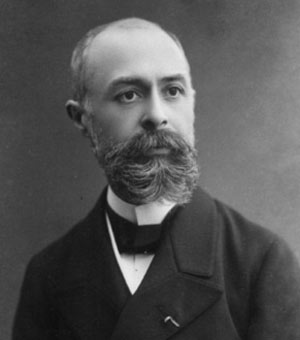
\includegraphics[width=0.92\textwidth]{images/becquerel.jpg}
\captionof{figure}{Henri Becquerel (1852--1908).}
\end{minipage}\hfill
\begin{minipage}{0.30\textwidth}
\centering
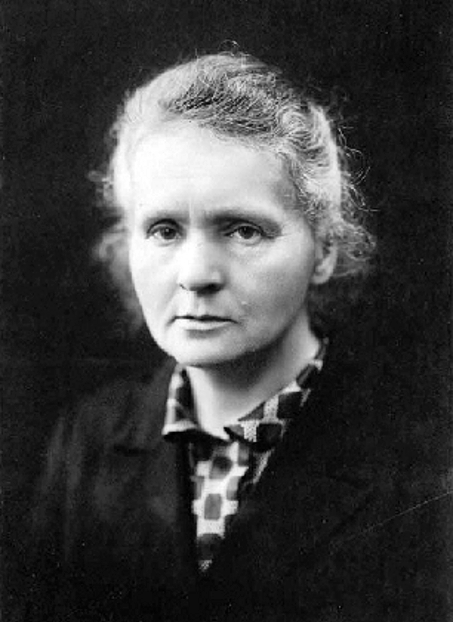
\includegraphics[width=0.92\textwidth]{images/curie.jpg}
\captionof{figure}{Marie Curie (1867--1934).}
\end{minipage}\hfill
\begin{minipage}{0.30\textwidth}
\centering
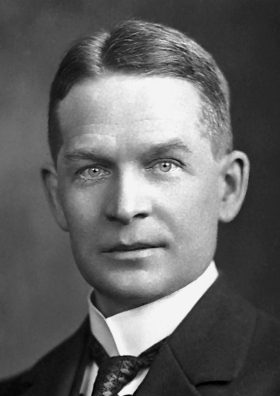
\includegraphics[width=0.92\textwidth]{images/soddy.jpg}
\captionof{figure}{Frederick Soddy (1877--1956).}
\end{minipage}

In 1896, French physicist Henri Becquerel accidentally discovered that uranium salts wrapped in opaque black paper spontaneously exposed photographic plates without sunlight. Marie Sk\l{}odowska-Curie coined the term \emph{radioactivity} and, alongside Pierre Curie, isolated the highly radioactive elements polonium and radium from pitchblende ore. In 1913, Frederick Soddy formulated the radioactive displacement laws, proving that radioactive decay transmutes one chemical element into another.
\end{historicalbox}

\section{Natural Radioactivity and Fundamental Decay Modes}

Unstable nuclei spontaneously decay via four primary physical mechanisms governed by nuclear instability (excess mass, excess neutrons, or excess protons):

\begin{figure}[htbp]
\centering
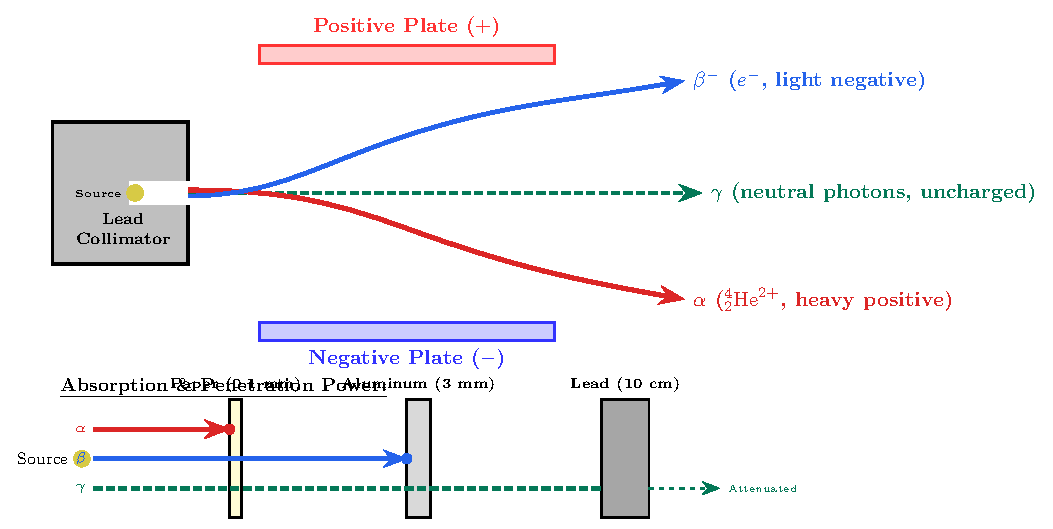
\includegraphics[width=0.88\textwidth]{figures/06_nuclear_deflection.pdf}
\caption{Top: Deflection of $\alpha$, $\beta^-$, and $\gamma$ rays in a transverse electric field. The heavy positive $\alpha$ particles bend gently toward the negative plate; light negative $\beta^-$ electrons bend sharply toward the positive plate; neutral $\gamma$ photons propagate undeflected. Bottom: Penetration power through paper ($0.1\ \mathrm{mm}$), aluminum ($3\ \mathrm{mm}$), and dense lead ($10\ \mathrm{cm}$).}
\label{fig:nuclear_deflection}
\end{figure}

\subsection{1. Alpha ($\alpha$) Disintegration}
Alpha decay occurs primarily in heavy radionuclides ($Z > 82, A > 200$) seeking to shed excess positive charge and mass. The parent nucleus expels a tightly bound Helium-4 nucleus ($\ce{^4_2He^{2+}}$):
\begin{equation}
\ce{^{A}_{Z}X -> ^{A-4}_{Z-2}Y + ^4_2He}.
\end{equation}
\begin{itemize}[leftmargin=1.5em,itemsep=2pt]
  \item \textbf{Displacement Law:} Mass number decreases by $4$ ($\Delta A = -4$); atomic number decreases by $2$ ($\Delta Z = -2$, shifting the element two columns to the left in the periodic table).
  \item \textbf{Canonical Example:} Alpha decay of Uranium-238 to Thorium-234:
  \[
  \ce{^{238}_{92}U -> ^{234}_{90}Th + ^4_2He}.
  \]
  \item \textbf{Physical Properties:} Alpha particles are massive ($m_\alpha \approx 4\ \mathrm{u}$) and carry charge $+2e$. They possess high linear energy transfer (LET) and intense ionizing power, but very low penetration: an ordinary sheet of paper ($0.1\ \mathrm{mm}$) or dead outer skin cells completely stops them.
\end{itemize}

\subsection{2. Beta-Minus ($\beta^-$) Disintegration}
Beta-minus decay occurs in **neutron-rich** nuclei located above the valley of nuclear stability ($N/Z$ ratio too high). Inside the nucleus, a neutron spontaneously converts into a proton via the weak nuclear interaction, emitting an energetic high-speed electron ($^0_{-1}e$) and an electron antineutrino ($\bar{\nu}_e$):
\begin{equation}
\ce{^1_0n -> ^1_1p + ^0_{-1}e + \bar{\nu}_e}.
\end{equation}
The nuclear transmutation equation is:
\begin{equation}
\ce{^{A}_{Z}X -> ^{A}_{Z+1}Y + ^0_{-1}e + \bar{\nu}_e}.
\end{equation}
\begin{itemize}[leftmargin=1.5em,itemsep=2pt]
  \item \textbf{Displacement Law:} Mass number remains invariant ($\Delta A = 0$); atomic number increases by $1$ ($\Delta Z = +1$, shifting the element one column to the right).
  \item \textbf{Canonical Example:} Beta decay of Carbon-14 into stable Nitrogen-14:
  \[
  \ce{^{14}_6C -> ^{14}_7N + ^0_{-1}e + \bar{\nu}_e}.
  \]
  \item \textbf{Physical Properties:} $\beta^-$ particles are electrons traveling at relativistic speeds ($v \sim 0.9\,c$). They penetrate several meters of air or several millimeters of biological tissue, but are halted by a thin aluminum plate ($3\text{--}5\ \mathrm{mm}$).
\end{itemize}

\subsection{3. Beta-Plus ($\beta^+$) Disintegration (Positron Emission)}
Beta-plus decay occurs in **proton-rich** nuclei located below the valley of stability ($N/Z$ ratio too low). A nuclear proton converts into a neutron, emitting a **positron** ($^0_{+1}e$, the antimatter counterpart of the electron) and an electron neutrino ($\nu_e$):
\begin{equation}
\ce{^1_1p -> ^1_0n + ^0_{+1}e + \nu_e}.
\end{equation}
The nuclear transmutation equation is:
\begin{equation}
\ce{^{A}_{Z}X -> ^{A}_{Z-1}Y + ^0_{+1}e + \nu_e}.
\end{equation}
\begin{itemize}[leftmargin=1.5em,itemsep=2pt]
  \item \textbf{Displacement Law:} Mass number remains invariant ($\Delta A = 0$); atomic number decreases by $1$ ($\Delta Z = -1$, shifting the element one column to the left).
  \item \textbf{Canonical Example:} Fluorine-18 decay utilized in Positron Emission Tomography (PET scans):
  \[
  \ce{^{18}_9F -> ^{18}_8O + ^0_{+1}e + \nu_e}.
  \]
  \item \textbf{Positron Annihilation:} Upon encountering an ambient orbital electron ($e^-$), the emitted positron undergoes immediate matter-antimatter annihilation, producing two diametrically opposed $511\ \mathrm{keV}$ gamma photons:
  \[
  \ce{^0_{+1}e + ^0_{-1}e -> 2\,\gamma} \quad (E_\gamma = m_e c^2 = 0.511\ \mathrm{MeV}).
  \]
\end{itemize}

\subsection{4. Gamma ($\gamma$) Electromagnetic De-excitation}
Following an $\alpha$ or $\beta$ transition, the daughter nucleus is frequently left in a quantum-mechanically excited metastable nuclear state, designated by an asterisk $[^{A}_{Z}\mathrm{Y}]^*$. The nucleus returns to its ground state by emitting one or more ultra-high-energy electromagnetic photons ($\gamma$-rays):
\begin{equation}
\ce{[^{A}_{Z}Y]^* -> ^{A}_{Z}Y + \gamma}.
\end{equation}
\begin{itemize}[leftmargin=1.5em,itemsep=2pt]
  \item \textbf{Displacement Law:} Neither mass number nor atomic number changes ($\Delta A = 0, \Delta Z = 0$). Gamma emission is a pure energetic de-excitation.
  \item \textbf{Physical Properties:} Gamma rays are uncharged electromagnetic photons of extremely short wavelength ($\lambda < 10^{-11}\ \mathrm{m}$) and high energy ($E_\gamma \sim 0.1\text{--}10\ \mathrm{MeV}$). They possess tremendous penetration power, requiring several centimeters of dense lead ($\mathrm{Pb}$) or several meters of reinforced concrete for radiation shielding.
\end{itemize}

\section{Conservation Laws in Nuclear Reactions (Soddy-Fajans Laws)}

Every nuclear transmutation, whether natural or artificially induced, obeys the strict **Soddy-Fajans conservation principles**:

\begin{lawbox}{The Soddy-Fajans Conservation Laws}
For any general nuclear reaction:
\begin{equation}
\ce{^{A_1}_{Z_1}X_1 + ^{A_2}_{Z_2}X_2 -> ^{A_3}_{Z_3}X_3 + ^{A_4}_{Z_4}X_4 + \dots}
\end{equation}
\begin{enumerate}[leftmargin=1.5em,itemsep=3pt]
  \item \textbf{Conservation of Nucleon Mass Number $A$:} The sum of mass numbers of the reactants equals the sum of mass numbers of the products:
  \begin{equation}
  \sum A_{\text{reactants}} = \sum A_{\text{products}} \iff A_1 + A_2 = A_3 + A_4 + \dots
  \end{equation}
  \item \textbf{Conservation of Electric Charge Number $Z$:} The algebraic sum of atomic numbers (nuclear charges) is strictly conserved:
  \begin{equation}
  \sum Z_{\text{reactants}} = \sum Z_{\text{products}} \iff Z_1 + Z_2 = Z_3 + Z_4 + \dots
  \end{equation}
  \item \textbf{Conservation of Total Relativistic Energy and Momentum:} Total energy (including rest mass energy $m c^2$) and total linear momentum are conserved.
\end{enumerate}
\end{lawbox}

\section{Artificial Nuclear Reactions and Transmutations}

Artificial nuclear reactions are induced by bombarding a stationary target nucleus with accelerated particles (protons, alpha particles, deuterons, or thermal neutrons).

\subsection{1. Compact Reaction Notation}
Nuclear reactions are frequently written in the condensed notation:
\begin{equation}
\text{Target Nuclide}\;(\text{Incident Projectile},\;\text{Ejected Particle})\;\text{Residual Nuclide}.
\end{equation}
\begin{itemize}[leftmargin=1.5em,itemsep=3pt]
  \item \textbf{Rutherford's Transmutation (1919):}
  \[
  \ce{^{14}_7N + ^4_2He -> ^{17}_8O + ^1_1p} \iff \ce{^{14}_7N}(\alpha, p)\ce{^{17}_8O}.
  \]
  \item \textbf{Chadwick's Neutron Discovery (1932):}
  \[
  \ce{^9_4Be + ^4_2He -> ^{12}_6C + ^1_0n} \iff \ce{^9_4Be}(\alpha, n)\ce{^{12}_6C}.
  \]
  \item \textbf{Joliot-Curie Artificial Radioactivity (1934):}
  \[
  \ce{^{27}_{13}Al + ^4_2He -> ^{30}_{15}P + ^1_0n} \iff \ce{^{27}_{13}Al}(\alpha, n)\ce{^{30}_{15}P}.
  \]
\end{itemize}

\subsection{2. Nuclear Fission}
Heavy fissile nuclides like Uranium-235 ($\ce{^{235}_{92}U}$) or Plutonium-239 ($\ce{^{239}_{94}Pu}$), when capturing a low-energy thermal neutron ($v \approx 2200\ \mathrm{m/s}$), form an unstable compound nucleus that violently ruptures into two lighter fission fragments and $2$ to $3$ fast secondary neutrons:
\begin{equation}
\ce{^{235}_{92}U + ^1_0n -> [^{236}_{92}U]^* -> ^{141}_{56}Ba + ^{92}_{36}Kr + 3\,^1_0n} + 200\ \mathrm{MeV}.
\end{equation}
Because the reaction produces more neutrons than it consumes ($k > 1$), it sustains an exponential **nuclear chain reaction**, harnessed constructively in nuclear power reactors or destructively in atomic weapons.

\subsection{3. Thermonuclear Fusion}
At extreme temperatures ($T \sim 10^8\ \mathrm{K}$), light nuclei overcome their repulsive Coulomb barrier to fuse into heavier, more tightly bound nuclei:
\begin{equation}
\ce{^2_1H + ^3_1H -> ^4_2He + ^1_0n} + 17.59\ \mathrm{MeV}.
\end{equation}
Thermonuclear fusion powers the Sun and main-sequence stars and represents the ultimate aspiration of clean commercial fusion energy research (ITER, tokamak reactors).

\section{Kinetics of Radioactive Decay}

Radioactive disintegration is a stochastic quantum process: it is impossible to predict when an individual nucleus will decay, but for a macroscopic sample containing $N(t)$ identical nuclei, the decay rate is strictly proportional to the number of parent nuclei present.

\subsection{1. The Law of Radioactive Decay}

\begin{lawbox}{First-Order Radioactive Decay Law}
The instantaneous disintegration rate of a radionuclide is governed by the first-order differential equation:
\begin{equation}
\frac{\dd N(t)}{\dd t} = -\lambda \cdot N(t),
\end{equation}
where $\lambda > 0$ is the **decay constant** (disintegration constant), representing the intrinsic probability of decay per nucleus per unit time ($[\lambda] = \mathrm{s^{-1}}, \mathrm{min^{-1}}, \mathrm{h^{-1}}, \mathrm{yr^{-1}}$).
\end{lawbox}

\paragraph{Mathematical Derivation.}
Separating variables:
\[
\frac{\dd N}{N} = -\lambda\,\dd t.
\]
Integrating both sides from $t = 0$ (where $N(0) = N_0$) to time $t$:
\[
\int_{N_0}^{N(t)} \frac{\dd N'}{N'} = -\lambda \int_0^t \dd t' \implies \ln\left( \frac{N(t)}{N_0} \right) = -\lambda t.
\]
Exponentiating both sides:
\begin{equation}
\mathbf{N(t) = N_0\,e^{-\lambda t}}.
\end{equation}

\begin{figure}[htbp]
\centering
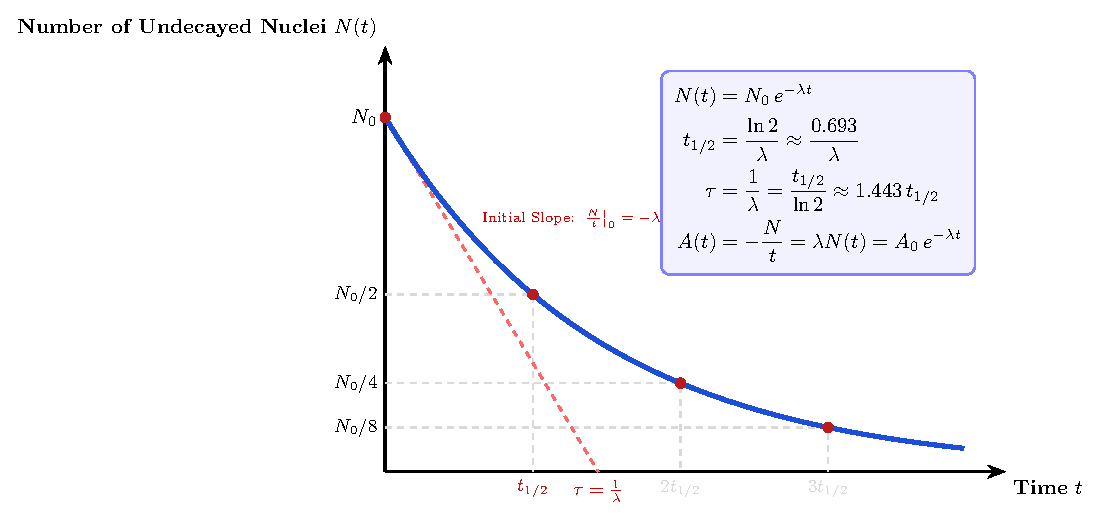
\includegraphics[width=0.88\textwidth]{figures/07_decay_kinetics.pdf}
\caption{Kinetics of radioactive decay. The population of undecayed nuclei decreases by half with every elapsed half-life $t_{1/2}$. The initial tangent line at $t=0$ intersects the time axis at the mean nuclear lifetime $\tau = 1/\lambda$.}
\label{fig:decay_kinetics}
\end{figure}

Because the mass $m(t)$ and amount of substance $n(t)$ of the radionuclide are directly proportional to particle count ($N = \frac{m}{M} N_A = n N_A$), the decay law applies identically to mass and moles:
\begin{equation}
m(t) = m_0\,e^{-\lambda t}, \qquad n(t) = n_0\,e^{-\lambda t}.
\end{equation}

\subsection{2. Radioactive Half-Life ($t_{1/2}$ or $T$)}

\begin{definitionbox}{Radioactive Half-Life}
The **radioactive half-life** $t_{1/2}$ (or \emph{period} $T$) is the time required for exactly one-half of the initial radioactive nuclei in a sample to disintegrate:
\begin{equation}
N(t_{1/2}) \eqdef \frac{N_0}{2}.
\end{equation}
\end{definitionbox}

Substituting into the decay law:
\[
\frac{N_0}{2} = N_0\,e^{-\lambda t_{1/2}} \implies e^{\lambda t_{1/2}} = 2 \implies \lambda \cdot t_{1/2} = \ln 2.
\]

\begin{lawbox}{Relationship Between Half-Life and Decay Constant}
\begin{equation}
\mathbf{t_{1/2} = \frac{\ln 2}{\lambda} \approx \frac{0.693\,147}{\lambda}}, \qquad \mathbf{\lambda = \frac{\ln 2}{t_{1/2}}}.
\end{equation}
After $k$ elapsed half-lives ($t = k \cdot t_{1/2}$), the remaining population is:
\begin{equation}
N(t) = N_0 \left(\frac{1}{2}\right)^k = \frac{N_0}{2^{t / t_{1/2}}}.
\end{equation}
\end{lawbox}

\subsection{3. Mean Nuclear Lifetime ($\tau$)}
The average lifetime of an individual radioactive nucleus before disintegration is:
\begin{equation}
\tau \eqdef \frac{1}{\lambda} = \frac{t_{1/2}}{\ln 2} \approx 1.4427 \cdot t_{1/2}.
\end{equation}
At time $t = \tau$, the population has dropped to $N(\tau) = N_0 / e \approx 0.3679\,N_0$ ($36.8\%$ remaining). Geometrically, $\tau$ is the intercept of the initial tangent line on the time axis (see Figure~\ref{fig:decay_kinetics}).

\section{Radioactive Activity ($A$) and Measurement Units}

\begin{definitionbox}{Radioactive Activity ($A$)}
The **radioactive activity** $A(t)$ of a sample is defined as the absolute rate of nuclear disintegrations occurring within the sample per unit time:
\begin{equation}
A(t) \eqdef -\frac{\dd N(t)}{\dd t} = \lambda \cdot N(t).
\end{equation}
At initial time $t = 0$: $A_0 = \lambda N_0$.
The activity decays following the identical exponential law:
\begin{equation}
\mathbf{A(t) = A_0\,e^{-\lambda t}}.
\end{equation}
\end{definitionbox}

\subsection{Units of Radioactivity}
\begin{itemize}[leftmargin=1.5em,itemsep=4pt]
  \item \textbf{The Becquerel ($\mathrm{Bq}$):} The official SI unit of radioactivity.
  \begin{equation}
  1\ \mathrm{Bq} \eqdef 1\ \text{disintegration per second}\ (\mathrm{dps}).
  \end{equation}
  \item \textbf{The Curie ($\mathrm{Ci}$):} Historical non-SI unit, originally defined as the activity of $1.00\ \mathrm{g}$ of pure Radium-226 ($\ce{^{226}_{88}Ra}$):
  \begin{equation}
  1\ \mathrm{Ci} \eqdef 3.7 \times 10^{10}\ \mathrm{Bq} = 3.7 \times 10^{10}\ \mathrm{dps} = 37\ \mathrm{GBq}.
  \end{equation}
  Decimal submultiples are universally used in medicine and industry:
  \begin{align*}
  1\ \mathrm{mCi} &= 10^{-3}\ \mathrm{Ci} = 3.7 \times 10^7\ \mathrm{Bq} = 37\ \mathrm{MBq}, \\
  1\ \mu\mathrm{Ci} &= 10^{-6}\ \mathrm{Ci} = 3.7 \times 10^4\ \mathrm{Bq} = 37\ \mathrm{kBq}.
  \end{align*}
\end{itemize}

\subsection{Specific Activity ($a_s$)}
The **specific activity** $a_s$ is the activity per unit mass of the pure radioactive isotope:
\begin{equation}
a_s \eqdef \frac{A}{m} = \frac{\lambda N}{m} = \frac{\lambda \left(\frac{m}{M} N_A\right)}{m} = \frac{\lambda N_A}{M} = \frac{\ln 2 \cdot N_A}{t_{1/2} \cdot M}, \qquad [a_s] = \mathrm{Bq\cdot g^{-1}} \quad (\text{or } \mathrm{Bq\cdot kg^{-1}}).
\end{equation}

\section{Applications of Radioactivity and Radiometric Dating}

\subsection{1. Archaeological Radiocarbon Dating ($^{14}\mathrm{C}$)}
Carbon-14 ($\ce{^{14}_6C}$) is continuously produced in the upper atmosphere by cosmic-ray neutrons bombarding Nitrogen-14:
\[
\ce{^{14}_7N + ^1_0n -> ^{14}_6C + ^1_1p}.
\]
The $^{14}\mathrm{C}$ rapidly oxidizes to $\ce{^{14}CO_2}$, entering the global biological carbon cycle through plant photosynthesis. In all living organisms, a dynamic metabolic equilibrium maintains a constant isotopic ratio:
\[
\left(\frac{\ce{^{14}C}}{\ce{^{12}C}}\right)_{\text{living}} \approx 1.2 \times 10^{-12} \iff A_0 \approx 15.3\ \text{disintegrations per minute per gram of carbon}\ (\mathrm{dpm\cdot g^{-1}}).
\]
When an organism dies, carbon assimilation abruptly ceases. The trapped $^{14}\mathrm{C}$ undergoes spontaneous $\beta^-$ decay ($t_{1/2} = 5730\ \mathrm{yr}$):
\[
\ce{^{14}_6C -> ^{14}_7N + ^0_{-1}e + \bar{\nu}_e}.
\]
Measuring the residual specific activity $A(t)$ of an archaeological specimen allows determination of its post-mortem age $t$:

\begin{lawbox}{Radiocarbon Age Equation}
\begin{equation}
t = \frac{1}{\lambda} \ln\left( \frac{A_0}{A(t)} \right) = \frac{t_{1/2}}{\ln 2} \ln\left( \frac{A_0}{A(t)} \right).
\end{equation}
\end{lawbox}

\subsection{2. Geological Rock Dating (Uranium-Lead Isochron)}
Uranium-238 ($\ce{^{238}U}$, $t_{1/2} = 4.468 \times 10^9\ \mathrm{yr}$) decays through a multi-step radioactive decay chain terminating at stable Lead-206 ($\ce{^{206}Pb}$):
\[
\ce{^{238}_{92}U -> ^{206}_{82}Pb + 8\,^4_2He + 6\,^0_{-1}e}.
\]
For a closed zircon crystal mineral that incorporated Uranium but zero initial Lead during magma crystallization:
\[
N(\ce{^{238}U}) = N_0\,e^{-\lambda t}, \qquad N(\ce{^{206}Pb}) = N_0 - N(\ce{^{238}U}) = N(\ce{^{238}U})(e^{\lambda t} - 1).
\]
The geological crystallization age of the rock is:
\begin{equation}
t = \frac{1}{\lambda} \ln\left( 1 + \frac{N(\ce{^{206}Pb})}{N(\ce{^{238}U})} \right).
\end{equation}

\section{Comprehensive Worked Examples}

\begin{workedexample}{Balancing Nuclear Transmutations and Decay Chains}
\begin{enumerate}[leftmargin=1.4em,itemsep=3pt]
  \item Identify the unknown particle or nuclide $\ce{X}$ in each of the following nuclear reactions:
  \begin{enumerate}[leftmargin=1.2em,itemsep=2pt]
    \item $\ce{^{226}_{88}Ra -> ^{222}_{86}Rn + X_1}$,
    \item $\ce{^{60}_{27}Co -> ^{60}_{28}Ni + X_2 + \bar{\nu}_e}$,
    \item $\ce{^{22}_{11}Na -> ^{22}_{10}Ne + X_3 + \nu_e}$,
    \item $\ce{^{235}_{92}U + ^1_0n -> ^{95}_{38}Sr + ^{139}_{54}Xe + X_4}$.
  \end{enumerate}
  \item The natural radioactive decay chain of Uranium-238 ($\ce{^{238}_{92}U}$) terminates at stable Lead-206 ($\ce{^{206}_{82}Pb}$) after a series of successive $\alpha$ and $\beta^-$ decays:
  \[
  \ce{^{238}_{92}U -> ^{206}_{82}Pb + x\,^4_2He + y\,^0_{-1}e}.
  \]
  Determine the exact integer number of alpha particles ($x$) and beta-minus particles ($y$) emitted throughout the entire chain.
\end{enumerate}

\paragraph{Solution.}
\textbf{1. Balancing Nuclear Reactions via Soddy-Fajans Laws:}\\
\begin{enumerate}[leftmargin=1.2em,itemsep=3pt]
  \item $\ce{^{226}_{88}Ra -> ^{222}_{86}Rn + X_1}$:
  Mass balance: $226 = 222 + A_1 \implies A_1 = 4$.
  Charge balance: $88 = 86 + Z_1 \implies Z_1 = 2$.
  $\mathbf{X_1 = \ce{^4_2He}}$ ($\alpha$ particle).
  \item $\ce{^{60}_{27}Co -> ^{60}_{28}Ni + X_2 + \bar{\nu}_e}$:
  Mass balance: $60 = 60 + A_2 \implies A_2 = 0$.
  Charge balance: $27 = 28 + Z_2 \implies Z_2 = -1$.
  $\mathbf{X_2 = \ce{^0_{-1}e}}$ ($\beta^-$ particle / electron).
  \item $\ce{^{22}_{11}Na -> ^{22}_{10}Ne + X_3 + \nu_e}$:
  Mass balance: $22 = 22 + A_3 \implies A_3 = 0$.
  Charge balance: $11 = 10 + Z_3 \implies Z_3 = +1$.
  $\mathbf{X_3 = \ce{^0_{+1}e}}$ ($\beta^+$ particle / positron).
  \item $\ce{^{235}_{92}U + ^1_0n -> ^{95}_{38}Sr + ^{139}_{54}Xe + X_4}$:
  Reactants: $\sum A = 235 + 1 = 236$; $\sum Z = 92 + 0 = 92$.
  Products (known): $\sum A = 95 + 139 = 234$; $\sum Z = 38 + 54 = 92$.
  Missing mass: $A_4 = 236 - 234 = 2$. Missing charge: $Z_4 = 92 - 92 = 0$.
  Because free neutrons have $A = 1, Z = 0$, the missing piece corresponds to two free neutrons:
  $\mathbf{X_4 = 2\,\ce{^1_0n}}$.
\end{enumerate}

\textbf{2. Uranium-238 Decay Chain Disintegration Count:}\\
Applying the conservation equations to $\ce{^{238}_{92}U -> ^{206}_{82}Pb + x\,^4_2He + y\,^0_{-1}e}$:
\begin{itemize}[leftmargin=1.5em,itemsep=2pt]
  \item Conservation of mass number $A$:
  \[
  238 = 206 + 4x + 0y \implies 4x = 238 - 206 = 32 \implies \mathbf{x = 8}.
  \]
  Exactly **$8$ alpha particles** are emitted!
  \item Conservation of charge number $Z$:
  \[
  92 = 82 + 2x - 1y.
  \]
  Substituting $x = 8$:
  \[
  92 = 82 + 2(8) - y = 82 + 16 - y = 98 - y \implies y = 98 - 92 \implies \mathbf{y = 6}.
  \]
  Exactly **$6$ beta-minus particles** are emitted!
\end{itemize}
The complete net decay chain is:
\[
\ce{^{238}_{92}U -> ^{206}_{82}Pb + 8\,^4_2He + 6\,^0_{-1}e + 6\,\bar{\nu}_e}.
\]
\end{workedexample}

\begin{workedexample}{Kinetics, Activity, and Attenuation of a Cobalt-60 Teletherapy Source}
Cobalt-60 ($\ce{^{60}_{27}Co}$) is a standard radionuclide used in industrial radiography and medical cancer radiation therapy. Its radioactive half-life is $t_{1/2} = 5.271\ \mathrm{years}$. A newly manufactured hospital radiotherapy head contains an initial Cobalt-60 activity $A_0 = 4000\ \mathrm{Ci}$.
\begin{enumerate}[leftmargin=1.4em,itemsep=3pt]
  \item Compute the radioactive decay constant $\lambda$ of Cobalt-60 in $\mathrm{s^{-1}}$ and in $\mathrm{yr^{-1}}$.
  \item Calculate the initial mass $m_0$ of pure Cobalt-60 in the source ($M = 59.9338\ \mathrm{g\cdot mol^{-1}}$).
  \item Determine the residual activity $A(t)$ (in $\mathrm{Ci}$ and in $\mathrm{TBq}$) after $3.00\ \mathrm{years}$ of clinical operation.
  \item Calculate the time $t$ required for the activity to decline to $1000\ \mathrm{Ci}$ (a factor of $4$ reduction).
\end{enumerate}

\paragraph{Solution.}
\textbf{1. Decay Constant $\lambda$:}\\
Using $1\ \mathrm{yr} = 365.25\ \mathrm{d} \times 86\,400\ \mathrm{s/d} = 3.15576 \times 10^7\ \mathrm{s}$:
\[
\lambda\ [\mathrm{yr^{-1}}] = \frac{\ln 2}{t_{1/2}} = \frac{0.693\,147}{5.271\ \mathrm{yr}} \approx \mathbf{0.13150\ \mathrm{yr^{-1}}}.
\]
In SI units:
\[
\lambda\ [\mathrm{s^{-1}}] = \frac{0.13150\ \mathrm{yr^{-1}}}{3.15576 \times 10^7\ \mathrm{s\cdot yr^{-1}}} \approx \mathbf{4.167 \times 10^{-9}\ \mathrm{s^{-1}}}.
\]

\textbf{2. Initial Mass of the Source:}\\
Convert the initial activity from Curies to Becquerels ($1\ \mathrm{Ci} = 3.7 \times 10^{10}\ \mathrm{Bq}$):
\[
A_0 = 4000\ \mathrm{Ci} \times 3.7 \times 10^{10}\ \mathrm{Bq\cdot Ci^{-1}} = 1.480 \times 10^{14}\ \mathrm{Bq} = 148.0\ \mathrm{TBq}.
\]
Since $A_0 = \lambda N_0$, the number of $\ce{^{60}Co}$ nuclei is:
\[
N_0 = \frac{A_0}{\lambda} = \frac{1.480 \times 10^{14}\ \mathrm{s^{-1}}}{4.167 \times 10^{-9}\ \mathrm{s^{-1}}} \approx 3.5517 \times 10^{22}\ \text{nuclei}.
\]
The initial mass of pure Cobalt-60 is:
\[
m_0 = \frac{N_0}{N_A} \times M = \frac{3.5517 \times 10^{22}}{6.02214 \times 10^{23}\ \mathrm{mol^{-1}}} \times 59.9338\ \mathrm{g\cdot mol^{-1}} \approx \mathbf{3.535\ \mathrm{g}}.
\]
A minuscule sample of only $3.54\ \mathrm{g}$ produces a colossal radiation activity of $4000\ \mathrm{Ci}$!

\textbf{3. Activity After $3.00\ \mathrm{Years}$:}\\
Applying the exponential decay law $A(t) = A_0\,e^{-\lambda t}$:
\[
A(3.00\ \mathrm{yr}) = 4000\ \mathrm{Ci} \times e^{-0.13150 \times 3.00} = 4000 \times e^{-0.3945} = 4000 \times 0.6740 \approx \mathbf{2696\ \mathrm{Ci}}.
\]
In Terabecquerels:
\[
A(3.00\ \mathrm{yr}) = 2696\ \mathrm{Ci} \times 3.7 \times 10^{10}\ \mathrm{Bq\cdot Ci^{-1}} \approx \mathbf{99.75\ \mathrm{TBq}}.
\]

\textbf{4. Time for Activity to Drop to $1000\ \mathrm{Ci}$:}\\
Notice that:
\[
\frac{A(t)}{A_0} = \frac{1000}{4000} = \frac{1}{4} = \left(\frac{1}{2}\right)^2.
\]
Because the activity drops by a factor of 4, exactly $k = 2$ half-lives have elapsed:
\[
t = 2 \times t_{1/2} = 2 \times 5.271\ \mathrm{yr} = \mathbf{10.542\ \mathrm{years}}.
\]
The source activity drops to $25\%$ in approximately $10.5$ years.
\end{workedexample}

\begin{workedexample}{Archaeological Radiocarbon Dating of an Ancient Artifact}
During an archaeological excavation of an ancient royal tomb, researchers discover a fragment of wooden furniture. A $1.00\ \mathrm{g}$ sample of purified elemental carbon extracted from the wood displays a measured beta activity of $4.18\ \text{disintegrations per minute}\ (\mathrm{dpm})$. Modern living tree wood displays a standard equilibrium carbon-14 activity of $A_0 = 15.30\ \mathrm{dpm\cdot g^{-1}}$. The half-life of Carbon-14 is $t_{1/2} = 5730\ \mathrm{years}$.
\begin{enumerate}[leftmargin=1.4em,itemsep=3pt]
  \item Determine the decay constant $\lambda$ of Carbon-14.
  \item Calculate the age of the wooden artifact and determine the historical era of the burial.
  \item What percentage of the initial Carbon-14 nuclei remains undecayed?
\end{enumerate}

\paragraph{Solution.}
\textbf{1. Decay Constant $\lambda$:}\\
\[
\lambda = \frac{\ln 2}{t_{1/2}} = \frac{0.693\,147}{5730\ \mathrm{yr}} \approx \mathbf{1.2097 \times 10^{-4}\ \mathrm{yr^{-1}}}.
\]

\textbf{2. Age of the Artifact:}\\
The measured specific activity is $A(t) = 4.18\ \mathrm{dpm\cdot g^{-1}}$, while the initial activity at the moment the tree was felled was $A_0 = 15.30\ \mathrm{dpm\cdot g^{-1}}$.
Applying the radiocarbon dating equation:
\[
A(t) = A_0\,e^{-\lambda t} \implies \frac{A(t)}{A_0} = e^{-\lambda t} \implies \ln\left( \frac{A(t)}{A_0} \right) = -\lambda t.
\]
Solving for the elapsed time $t$:
\[
t = \frac{1}{\lambda} \ln\left( \frac{A_0}{A(t)} \right) = \frac{1}{1.2097 \times 10^{-4}\ \mathrm{yr^{-1}}} \ln\left( \frac{15.30}{4.18} \right).
\]
Evaluating the natural logarithm:
\[
\frac{15.30}{4.18} \approx 3.6603 \implies \ln(3.6603) \approx 1.2975.
\]
The age of the wood is:
\[
t = \frac{1.2975}{1.2097 \times 10^{-4}} \approx \mathbf{10\,726\ \mathrm{years}}.
\]
The tree was harvested approximately $10\,700$ years ago (circa $8700\ \text{BCE}$), during the Neolithic period.

\textbf{3. Percentage of Undecayed $^{14}\mathrm{C}$ Remaining:}\\
The fraction remaining is:
\[
\frac{N(t)}{N_0} = \frac{A(t)}{A_0} = \frac{4.18}{15.30} \approx 0.2732 = \mathbf{27.32\%}.
\]
Approximately $72.68\%$ of the original Carbon-14 nuclei have disintegrated.
\end{workedexample}

\begin{workedexample}{Geological Geochronology: Uranium-Lead Mineral Dating}
A geologist analyzes a pristine zircon ($\mathrm{ZrSiO_4}$) crystal extracted from an ancient granite rock formation. High-precision thermal ionization mass spectrometry (TIMS) measures the present-day atom ratio of radiogenic Lead-206 to parent Uranium-238:
\[
\frac{N(\ce{^{206}Pb})}{N(\ce{^{238}U})} = 0.4280.
\]
Assuming the crystal contained no initial Lead at the time of magma solidification, and that no Uranium or Lead has leaked from the crystal lattice, calculate the geological crystallization age of the rock ($t_{1/2}(\ce{^{238}U}) = 4.468 \times 10^9\ \mathrm{years}$).

\paragraph{Solution.}
\textbf{1. Theoretical Geochronology Derivation:}\\
Each decayed $\ce{^{238}U}$ atom produces exactly one stable $\ce{^{206}Pb}$ atom:
\[
N_0 = N(\ce{^{238}U}) + N(\ce{^{206}Pb}).
\]
The remaining Uranium-238 population follows the decay law:
\[
N(\ce{^{238}U}) = N_0\,e^{-\lambda t}.
\]
Substituting $N_0$:
\[
N(\ce{^{238}U}) = \left[ N(\ce{^{238}U}) + N(\ce{^{206}Pb}) \right] e^{-\lambda t}.
\]
Dividing by $e^{-\lambda t}$ (multiplying by $e^{\lambda t}$):
\[
N(\ce{^{238}U})\,e^{\lambda t} = N(\ce{^{238}U}) + N(\ce{^{206}Pb}) \implies e^{\lambda t} = 1 + \frac{N(\ce{^{206}Pb})}{N(\ce{^{238}U})}.
\]
Taking the natural logarithm:
\[
\lambda t = \ln\left( 1 + \frac{N(\ce{^{206}Pb})}{N(\ce{^{238}U})} \right) \implies t = \frac{1}{\lambda} \ln\left( 1 + \frac{N(\ce{^{206}Pb})}{N(\ce{^{238}U})} \right).
\]

\textbf{2. Numerical Age Computation:}\\
The decay constant for Uranium-238 is:
\[
\lambda = \frac{\ln 2}{4.468 \times 10^9\ \mathrm{yr}} \approx 1.55135 \times 10^{-10}\ \mathrm{yr^{-1}}.
\]
The measured isotopic ratio is $0.4280$:
\[
1 + \frac{N(\ce{^{206}Pb})}{N(\ce{^{238}U})} = 1 + 0.4280 = 1.4280.
\]
Evaluating the natural logarithm:
\[
\ln(1.4280) \approx 0.356275.
\]
The age of the granite zircon crystal is:
\[
t = \frac{0.356275}{1.55135 \times 10^{-10}\ \mathrm{yr^{-1}}} \approx \mathbf{2.296 \times 10^9\ \mathrm{years}} = \mathbf{2.30\ \mathrm{billion\ years}}.
\]
The zircon crystal crystallized $2.30$ billion years ago during the Paleoproterozoic era of Earth's history.
\end{workedexample}


\appendix
\chapter{Reference Tables and Fundamental Data}
\label{app:tables}

\section{Fundamental Physical and Nuclear Constants}

\renewcommand{\arraystretch}{1.25}
\begin{longtable}{@{}llll@{}}
\toprule
\textbf{Physical Constant} & \textbf{Symbol} & \textbf{Recommended CODATA Value} & \textbf{SI Unit} \\
\midrule
\endhead
Speed of light in vacuum & $c$ & $2.997\,924\,58 \times 10^8$ & $\mathrm{m\cdot s^{-1}}$ (exact) \\
Avogadro's constant & $N_A$ & $6.022\,140\,76 \times 10^{23}$ & $\mathrm{mol^{-1}}$ (exact) \\
Elementary charge & $e$ & $1.602\,176\,634 \times 10^{-19}$ & $\mathrm{C}$ (exact) \\
Electronvolt & $1\ \mathrm{eV}$ & $1.602\,176\,634 \times 10^{-19}$ & $\mathrm{J}$ (exact) \\
Mega-electronvolt & $1\ \mathrm{MeV}$ & $1.602\,176\,634 \times 10^{-13}$ & $\mathrm{J}$ (exact) \\
Unified atomic mass unit & $1\ \mathrm{u} = 1/N_A$ & $1.660\,539\,066\,60 \times 10^{-27}$ & $\mathrm{kg}$ \\
Energy equivalent of $1\ \mathrm{u}$ & $1\ \mathrm{u} \cdot c^2$ & $931.494\,102$ & $\mathrm{MeV}$ \\
Proton rest mass & $m_p$ & $1.672\,621\,923\,69 \times 10^{-27}$ & $\mathrm{kg}$ \\
& & $1.007\,276\,466\,62$ & $\mathrm{u}$ \\
& & $938.272\,088$ & $\mathrm{MeV}/c^2$ \\
Neutron rest mass & $m_n$ & $1.674\,927\,498\,04 \times 10^{-27}$ & $\mathrm{kg}$ \\
& & $1.008\,664\,915\,95$ & $\mathrm{u}$ \\
& & $939.565\,420$ & $\mathrm{MeV}/c^2$ \\
Electron rest mass & $m_e$ & $9.109\,383\,7015 \times 10^{-31}$ & $\mathrm{kg}$ \\
& & $0.000\,548\,579\,909$ & $\mathrm{u}$ \\
& & $0.510\,998\,950$ & $\mathrm{MeV}/c^2$ \\
Neutral Hydrogen atom & $m(\ce{^1_1H})$ & $1.007\,825\,032$ & $\mathrm{u}$ \\
Molar gas constant & $R$ & $8.314\,462\,618$ & $\mathrm{J\cdot mol^{-1}\cdot K^{-1}}$ (exact) \\
Molar volume at STP & $V_m$ & $22.413\,962$ & $\mathrm{L\cdot mol^{-1}}$ \\
Curie unit & $1\ \mathrm{Ci}$ & $3.7 \times 10^{10}$ & $\mathrm{Bq}$ (exact) \\
\bottomrule
\end{longtable}

\section{Standard Isotopic Rest Masses}

\renewcommand{\arraystretch}{1.25}
\begin{longtable}{@{}lllll@{}}
\toprule
\textbf{Element} & \textbf{Nuclide} & \textbf{Atomic Rest Mass (u)} & \textbf{Natural Abundance (\%)} & \textbf{Half-Life ($t_{1/2}$)} \\
\midrule
\endhead
Hydrogen & $\ce{^1_1H}$ & $1.007\,825$ & $99.985\%$ & Stable \\
& $\ce{^2_1H}$ ($\mathrm{D}$) & $2.014\,102$ & $0.015\%$ & Stable \\
& $\ce{^3_1H}$ ($\mathrm{T}$) & $3.016\,049$ & Trace & $12.32\ \mathrm{yr}$ \\
Helium & $\ce{^3_2He}$ & $3.016\,029$ & $0.000\,14\%$ & Stable \\
& $\ce{^4_2He}$ & $4.002\,603$ & $99.999\,86\%$ & Stable \\
Lithium & $\ce{^6_3Li}$ & $6.015\,122$ & $7.59\%$ & Stable \\
& $\ce{^7_3Li}$ & $7.016\,004$ & $92.41\%$ & Stable \\
Beryllium & $\ce{^9_4Be}$ & $9.012\,182$ & $100\%$ & Stable \\
Boron & $\ce{^{10}_5B}$ & $10.012\,937$ & $19.9\%$ & Stable \\
& $\ce{^{11}_5B}$ & $11.009\,305$ & $80.1\%$ & Stable \\
Carbon & $\ce{^{12}_6C}$ & $12.000\,000$ (exact) & $98.93\%$ & Stable (standard) \\
& $\ce{^{13}_6C}$ & $13.003\,355$ & $1.07\%$ & Stable \\
& $\ce{^{14}_6C}$ & $14.003\,242$ & Trace & $5730\ \mathrm{yr}$ \\
Nitrogen & $\ce{^{14}_7N}$ & $14.003\,074$ & $99.63\%$ & Stable \\
& $\ce{^{15}_7N}$ & $15.000\,109$ & $0.37\%$ & Stable \\
Oxygen & $\ce{^{16}_8O}$ & $15.994\,915$ & $99.76\%$ & Stable \\
& $\ce{^{17}_8O}$ & $16.999\,132$ & $0.04\%$ & Stable \\
& $\ce{^{18}_8O}$ & $17.999\,160$ & $0.20\%$ & Stable \\
Chlorine & $\ce{^{35}_{17}Cl}$ & $34.968\,853$ & $75.76\%$ & Stable \\
& $\ce{^{37}_{17}Cl}$ & $36.965\,903$ & $24.24\%$ & Stable \\
Iron & $\ce{^{56}_{26}Fe}$ & $55.934\,937$ & $91.75\%$ & Stable ($E_L/A$ peak) \\
Uranium & $\ce{^{235}_{92}U}$ & $235.043\,929$ & $0.720\%$ & $7.04 \times 10^8\ \mathrm{yr}$ \\
& $\ce{^{238}_{92}U}$ & $238.050\,788$ & $99.274\%$ & $4.468 \times 10^9\ \mathrm{yr}$ \\
\bottomrule
\end{longtable}

\section{Master Solution Concentration Formula Summary}

\begin{center}
\renewcommand{\arraystretch}{1.4}
\begin{tabular}{@{}llll@{}}
\toprule
\textbf{Concentration Type} & \textbf{Symbol} & \textbf{Defining Formula} & \textbf{Common Units} \\
\midrule
Molarity & $C_M$ & $C_M = \dfrac{n_{\text{solute}}}{V_{\text{solution}}} = \dfrac{m}{M \cdot V}$ & $\mathrm{mol\cdot L^{-1}} \equiv \mathrm{M}$ \\
Mass Concentration & $C_m$ & $C_m = \dfrac{m_{\text{solute}}}{V_{\text{solution}}} = C_M \cdot M$ & $\mathrm{g\cdot L^{-1}}$ \\
Molality & $m$ & $m = \dfrac{n_{\text{solute}}}{m_{\text{solvent (kg)}}}$ & $\mathrm{mol\cdot kg^{-1}}$ \\
Normality & $N$ & $N = C_M \cdot Z$ & $\mathrm{eq\cdot L^{-1}} \equiv \mathrm{N}$ \\
Commercial Molarity & $C_M$ & $C_M = \dfrac{10 \cdot P\% \cdot d}{M}$ & $\mathrm{M}$ \\
Dilution Invariant & --- & $C_1 V_1 = C_2 V_2$ & --- \\
Titration Equivalence & --- & $N_1 V_1 = N_2 V_2$ & --- \\
\bottomrule
\end{tabular}
\end{center}


\end{document}
